\documentclass[a4paper,12pt]{article}
\usepackage[english]{babel}
\usepackage[utf8]{inputenc}
\usepackage{t1enc}
%\usepackage[T1]{fontenc}
\usepackage{floatflt}
\usepackage{graphicx}
\usepackage{psfrag}
\usepackage{bbm}
\usepackage{amsmath}
\usepackage{amssymb}
\usepackage{slashed}
%\usepackage{showkeys}
\usepackage{hyperref}
\usepackage{ifthen}
\usepackage{subcaption}
\usepackage{epstopdf}
\usepackage{enumerate}
\usepackage{dutchcal}
\usepackage{centernot}



\hoffset=-5.0mm
\voffset=-1.9mm
%
\evensidemargin=0cm
\oddsidemargin=0cm
\topmargin=0cm%
\headheight=0cm%
\headsep=0cm%
\marginparsep=0cm%
\marginparwidth=0cm%
\textheight=24cm
\textwidth=17cm
\special{papersize=210mm,297mm}%

\def\d{\mathrm{d}}
\def\e{\mathrm{e}}
\def\imagi{\mathrm{i}}
\def\ellop{\mathop{{\sf L}}}
\def\forrasfile#1{ (see {\tt #1})}
\def\lag{{\mathcal{L}}}
\def\lap{\mathop{\Delta}}
\def\kihagy#1{}
\def\sn{\mathop{\text{sn}}}
\def\cn{\mathop{\text{cn}}}
\def\dn{\mathop{\text{dn}}}
\def\zb{\ensuremath{\bar{z}}}
\def\sign{\mathop{\text{sign}}}
\def\xii#1{\xi^{(#1)}}
\def\xij#1#2{{\xi^{(#1)}_{#2}}}
\def\op#1{{\sf #1}}
\def\tphi{\ensuremath{\tilde{\phi}}}
\def\tphi{\ensuremath{\tilde{\phi}}}
\renewcommand\Re{\mathop{\text{Re}}}
\renewcommand\Im{\mathop{\text{Im}}}
\def\Tr{\ensuremath{\mathop{\rm Tr}}}
\def\pa{\partial}


\newcommand{\doi}[1]{\href{http://dx.doi.org/#1}{DOI: #1}}%
\newcommand{\doix}[2]{\href{http://dx.doi.org/#2}{#1}}%
\newcommand{\arxiv}[2][]{%
  \ifthenelse{\equal{#1}{}}{%
    \href{http://arxiv.org/abs/#2}{\texttt{arXiv:#2}}%
  }{%
    \href{http://arxiv.org/abs/#2}{\texttt{arXiv:#2 [#1]}}%
  }%
}%


\newcommand{\problem}[1]{\paragraph{Problem #1}}

%opening
\title{Geometry of physics - problem solutions}
\author{Árpád Lukács}

\begin{document}
\counterwithout{subsection}{section}

\maketitle

These are solutions to problems in Ref.\ \cite{Frankel}.


\section{Manifolds, tensors, and exterior forms}

\subsection{Manifolds and vector fields}

%%%%%%%%%%%%%%%%%%%%%%%%%%%%%%%%%%%%%%%%%%%%%%%%%%%%%%%%%%%%%%%%%%

\problem{1.1(1)} The locus $x^2 + y^2 - z^2 = c$ in $\mathbb{R}^3$ for $c <,=,> 0$:
\begin{itemize}
\item For $c<0$: Can reparametrise as $z = \pm \sqrt{x^2 + y^2 - c}$. A smooth manifold of two components: a two-sheeted hyperboloid.
\item For $x=0$: this is a cone, $z=\sqrt{x^2+y^2}$. Union of a manifold and $\{0\}$. If we omit the origin, we obtain a (non-connected) manifold. 
\item For $c>0$: $x^2 + y^2 = c + z^2$, can be parametrised as $(x,y) = \sqrt{c+z^2}(\cos\theta, \sin{\theta})$, a manifold: a one-sheeted hyperboloid.
\end{itemize}

%%%%%%%%%%%%%%%%%%%%%%%%%%%%%%%%%%%%%%%%%%%%%%%%%%%%%%%%%%%%%%%%%%

\problem{1.1(2)} ${\rm SO}(n)$ is a submanifold of $\mathbb{R}^{3\times 3}$, and a zero of one function $R\to R^T R -1$, into ${\rm Sym}^{n(n+1)/2}$, the set of symmetric $n\times n$ matrices, therefore a submanifold of dimension $n^2 - n(n+1)/2 = n(n-1)/2$.
As $(\det R)^2 = \det R^T R = 1$, the determinant condition only selects one component.

%%%%%%%%%%%%%%%%%%%%%%%%%%%%%%%%%%%%%%%%%%%%%%%%%%%%%%%%%%%%%%%%%%

\problem{1.1(3)} Yes, as $\det (R+\delta r) = \det R (1 + R^{-1}\delta r) = (\det R)\Tr \delta r$, the derivative of the determinant is $\op{D}\det [R] = (\det R)\Tr$, which, restricted to $SL(n)$ is the trace, a linear mapping of rank 1, therefore $GL(n)$ is an $n^2-1$ dimensional submanifold of $\mathbb{R}^{n\times n}$.

%%%%%%%%%%%%%%%%%%%%%%%%%%%%%%%%%%%%%%%%%%%%%%%%%%%%%%%%%%%%%%%%%%

\problem{1.1(4)} The $x$ component of the cross product is $\partial_y F \partial_z G - \partial_z F \partial_y G$. If this is non-vanishing, we can solve for $\d y/\d x$ and $\d z/\d x$ for a curve $x, y(x), z(x)$ locally from the equations: their derivatives are $\partial_x F + \partial_y F \d y/\d x + \partial_z F\d z/\d x = 0 $ and $\partial_x G + \partial_y G \d y/\d x + \partial_z G\d z/\d x = 0 $, expressed with the partial derivatives $\partial_x F$ and $\partial_x G$.

%%%%%%%%%%%%%%%%%%%%%%%%%%%%%%%%%%%%%%%%%%%%%%%%%%%%%%%%%%%%%%%%%%

\problem{1.2(1)} Let $U_{x}$ be those lines that do not lie in the $yz$ plane. These can be parameterised as $(y/x, z/x)$. Similarly, define $U_y$, $U_z$. A line in $U_x$ is then coordinatised as $x^1 = y/x$, $x^2 = z/x$, $[\lambda,\lambda x^1, \lambda x^2]$. The same line has coordinates $y^1 = x/y= 1/x^1$, $y^2=z/y = x^2/x^1$. Differentiable on the intersection. Similarly for the other transition functions.

%%%%%%%%%%%%%%%%%%%%%%%%%%%%%%%%%%%%%%%%%%%%%%%%%%%%%%%%%%%%%%%%%%

\problem{1.2(2)} Let $\mathbb{R}^{n-1} \ni (\xi^1, \dots, \xi^n)$, and a line in it is $[\lambda \xi^1, \dots, \lambda \xi^2]$ for $\lambda \in \mathbb{R}$. Let $U_i = \{ \xi^i \ne 0\}$. Coordinates: $\xi^j/\xi^i$, $i\ne j$. Transition function for two as above, e.g.,
let the coordinates be $x^1, \dots, x^{n-1}$ for $U_i$ and $y^1, \dots, y^{n-1}$ for $U_j$. Then a line in $\mathbb{C}^n$ is given as $\xi^k = \lambda x^k$ ($k <i$), $\xi^l = \lambda x^{k-1}$ ($k \ge i$) and $\xi^i = \lambda$, and then
$y^\ell = x^\ell / x^j$ for $\ell < i,j$, differentiable. The formula is similar for other values for $\ell$, indices are shifted.

%%%%%%%%%%%%%%%%%%%%%%%%%%%%%%%%%%%%%%%%%%%%%%%%%%%%%%%%%%%%%%%%%%

\problem{1.2(3)} Same. $\mathbb{C}P^1$ is the Riemann sphere.

%%%%%%%%%%%%%%%%%%%%%%%%%%%%%%%%%%%%%%%%%%%%%%%%%%%%%%%%%%%%%%%%%%

\problem{1.3(1)} It is coordinate system independent. If $x^i$ are coorinates, so are $y^i = \alpha x^i$ for some $0\ne \alpha \in \mathbb{R}$, yielding in $\|X\|^2_y = \|X\|^2_x / \alpha^2$, proving that the expression is not coordinate independent.

%%%%%%%%%%%%%%%%%%%%%%%%%%%%%%%%%%%%%%%%%%%%%%%%%%%%%%%%%%%%%%%%%%

\problem{1.3(2)} The two equatiorial circles, where the Jacobian becomes rank 1.

%%%%%%%%%%%%%%%%%%%%%%%%%%%%%%%%%%%%%%%%%%%%%%%%%%%%%%%%%%%%%%%%%%

\problem{1.3(3)} If $f_*$ is not onto to $\mathbb{R}$, it must vanish (as it is a number). On the other hand, $f_*$ is nothing but the restriction of the gradient to the tangent manifold, i.e., at a point $x\in M$,
\[
f_{*x} : T_x M \to \mathbb{R}, f_{*x} {\bf v} = \d f(x + {\bf v}t) / \d t|_{t=0} = \sum_i v^i \partial_i f(x)\,,
\]
and
\[
\partial_i f = \partial_i \sum_i (x^i)^2 = 2 x^i\,,
\]
i.e., for $x$ to be a critical point, the position vector must be orthogonal to all ${\bf v}$ in the tangent space (which is the definition of being orthogonal to the submanifold).

%%%%%%%%%%%%%%%%%%%%%%%%%%%%%%%%%%%%%%%%%%%%%%%%%%%%%%%%%%%%%%%%%%

\problem{1.4(1)} the solution to the differential equation is obtained as $\d x / x^2 = \d t$, i.e., $-1/x = t - t_0$, or $x(t) = -1/(t-t_0)$, and solvind the initial condition, $x(0) = 1/t_0 = p$ yields $\Phi_p(t) = -1/(t-1/p)$, which is defined for $-\infty < t < 1/p$,
or, in the case of $1/2 < x < 3/2$, the largest $\epsilon$ is 2/3.

%%%%%%%%%%%%%%%%%%%%%%%%%%%%%%%%%%%%%%%%%%%%%%%%%%%%%%%%%%%%%%%%%%

\problem{1.4(2)} The transition function is $w = 1/z$, and therefore $\dot w = -1/z^2 \dot z = -w^2$. The integral curves are $w(t) = 1/(t - 1/w_0) = w_0/(w_0 t -1)$. The point $w_0 = 0$ is a singular point, $\Phi_t(w_0 = 0) = 0$.

%%%%%%%%%%%%%%%%%%%%%%%%%%%%%%%%%%%%%%%%%%%%%%%%%%%%%%%%%%%%%%%%%%

\subsection{Tensors and exterior forms}

%%%%%%%%%%%%%%%%%%%%%%%%%%%%%%%%%%%%%%%%%%%%%%%%%%%%%%%%%%%%%%%%%%

\problem{2.1(1)} $\sum_j a_i^V v^i_V = \sum{ijk}(\partial x_V^i/\partial x_U^j) a_j^U (\partial x_U^k/\partial x_V^i) v_U^k = \sum_j a_j^U v^j_U$, the Jacobian matrix drops out. In the case of the two vectors, ${\bf v}$ and ${\bf w}$, the Jacobian components would remain in the sum (quadratically), the expression would not be coordinate invariant (unless the two coordinate systems are related to each other by an orthogonal matrix).

%%%%%%%%%%%%%%%%%%%%%%%%%%%%%%%%%%%%%%%%%%%%%%%%%%%%%%%%%%%%%%%%%%

\problem{2.1(2)} Using the chain rule, $\partial_r = \sin\vartheta\cos\varphi \partial_x + \sin\vartheta\sin\varphi \partial_y + \cos\vartheta \partial_z$, etc., yielding $g_{rr} = 1$, $g_{\vartheta\vartheta} = r^2$ and $g_{\varphi\varphi} = r^2 \sin^2\vartheta$, and all other components vanish.

The gradient vector components are calculated by raising the indices of the differential by using the inverse metric, i.e., $(\nabla f)^r = \partial f / \partial r$, $(\nabla f)^\vartheta = (1/r^2) \partial f/\partial \vartheta$, and $(\nabla f)^\varphi = (1/r^2/\sin^2\vartheta) \partial f/\partial\varphi^2$.

The primed unit vectors are ${\bf e}_j' = \partial_j / \sqrt{g_jj}$. In the usual formalism for orthonormal curvilinear coordinates, we denote $h_i^2 = g_{ii}$, and componets of th gradient are $(1/h_i)(\partial f/\partial x^i)$.

%%%%%%%%%%%%%%%%%%%%%%%%%%%%%%%%%%%%%%%%%%%%%%%%%%%%%%%%%%%%%%%%%%

\problem{2.3(1)} For the push-forward of any vector ${\bf v} = \sum_i v^i \partial/\partial x^i$, the following holds, $F_*{\bf v} = \sum_{i,j} v^i (\partial y^j/\partial x^i)(\partial / \partial y^j)$. Similarly, for ${\bf w} = \sum_j w^j (\partial/\partial y^j)$, $G_*{\bf w} = \sum_{j,k} w^j (\partial z^k/\partial y^j)\cdot (\partial / \partial z^k)$. Applying this to ${\bf w} = F_*{\bf v}$ and comparing that to applying $G\circ F$, and calculating its derivative using the chain rule yields the same.
%Using these results, and the fact that $(F^*\alpha){\bf v} = \alpha F_* {\bf v}$ for $\alpha \in T_x^* M$ and ${\bf v}]\in T_y W$, etc., yields the solution of the second part.

For the second part of the excercise: $\d x^i$ is defined by the relation $\d x^i (\partial/\partial x^j) = \delta^i_j$. Now let us consider $F^* \d y^j$. $(F^* \d y^j) (\partial/\partial x^i) = \d y^j F_* (\partial /\partial x^i) = \d y^j \sum (\partial y^k/\partial x^i) (\partial/\partial y^k) = \partial y^k/\partial x^i$. Proceed similarly to $G^* \d y^j$, and then compare with chain rule.

%%%%%%%%%%%%%%%%%%%%%%%%%%%%%%%%%%%%%%%%%%%%%%%%%%%%%%%%%%%%%%%%%%

\problem{2.3(2)} Let us first consider (i). Upon changing coordinates on $M$ from $q$ to $q'$, there is a change of coordinates on $TM$ from $q, \dot{q}$ to $\dot{q}, {\dot q}'$. Using the usual formula for the transformation of a vector in $TN$, there $N=TM$, we get
\[
\frac{\partial}{\partial q^i} = \sum_j \left( \frac{\partial {q'}^j}{\partial q^i}\frac{\partial}{\partial {q'}^j} + \frac{\partial \dot{q}{}'{}^j}{\partial q^i}\frac{\partial}{\partial \dot{q}{}'{}^j}\right)\,.
\]
To obtain the Jacobian components in the second term in the brackets, let us remember the transformation formula of vectors, applied to a vector $\sum_i {\dot q}^i \partial/\partial q^i$ (i.e., a point in $N=TM$):
\[
\dot{q}{}'{}^j = \sum_i \frac{\partial q'{}^j}{\partial q^i} \dot{q}{}^i\,,
\]
and calculating the second derivative yields
\[
\frac{\partial \dot{q}{}'{}^j}{\partial q^i} = \sum_k\frac{\partial^2 q'{}^j}{\partial q^i \partial q^k}\dot{q}{}^k\,.
\]

As for (ii), in another coordinate system
\[
\sum_i {\dot q}^i \frac{\partial}{\partial q^i} = \sum_{i,j} {\dot q}^i \left( \frac{\partial q'{}^j}{\partial q^i} \frac{\partial}{\partial q'{}^j} + \frac{\partial {\dot q}'{}^j}{\partial q^i}\frac{\partial}{\partial \dot{q}{}'{}^j}\right) = \sum_{ijk} \frac{\partial q^i}{\partial q'{}^k} \dot{q}{}^k \left( \frac{\partial q'{}^j}{\partial q^i} \frac{\partial}{\partial q'{}^j} + \frac{\partial {\dot q}'{}^j}{\partial q^i}\frac{\partial}{\partial \dot{q}{}'{}^j}\right)\,,
\]
and from (i), we see, that this is not well-defined globally: the first term in the brackets together with the Jacobian would yield the same expression in the primed coodinates as the one we started with in the unprimed ones, and the second term is additional and nonzero.

Similarly, for (iii),
\[
 \sum_i {\dot q}^i \frac{\partial}{\partial {\dot q}^i} = \sum_{ijk}  \frac{\partial q^i}{\partial q'{}^k} \dot{q}{}^k \left( \sum_l\frac{\partial^2 q'{}^l}{\partial q^j \partial q^l}\dot{q}^l \frac{\partial}{\partial q^j} + \frac{\partial q'{}^j}{\partial q^i}\frac{\partial}{\partial \dot{q}{}'{}^j} \right)\,,
\]
and in this case, the Jacobian components are cancelled from the second term and the pre-factor, yielding the same expression as the one we started with (but now in primed coordinates), and the first one is extra (in addition, we could express $\dot{q}{}^l$ in the new coordinates).

%%%%%%%%%%%%%%%%%%%%%%%%%%%%%%%%%%%%%%%%%%%%%%%%%%%%%%%%%%%%%%%%%%

\problem{2.4(1)} Compute: $\alpha \otimes \beta ({\bf v},{\bf w}) = \alpha({\bf v}) \beta({\bf w}) = \alpha(v^k \partial_k) \beta(w^\ell \partial_\ell) = v^k w^\ell \alpha(\partial_k) \beta(\partial_\ell) = v^k w^\ell a_i b_j \d x^i(\partial_k) \d x^j(\partial_\ell) = a_i b_k \d x^i(v^k \partial_k) x^j(w^\ell \partial_\ell) = a_i b_j \d x^i \otimes x^j (v^k \partial_k, w^\ell \partial_\ell) = a_i b_j \d x^i \otimes x^j ({\bf v}, {\bf w})$.

%%%%%%%%%%%%%%%%%%%%%%%%%%%%%%%%%%%%%%%%%%%%%%%%%%%%%%%%%%%%%%%%%%

\problem{2.4(2)} In a new (primed) basis, the matrix of the transformation is $A = J A J^{-1}$ where $J^i{}_j = \partial_j x'{}^i$ is the Jacobian. Using the cyclic property of the trace, $J$ is cancelled. On the other hand, for a covariant tensor, $J^{-1}J^{-1T}$ remains in the trace.

%%%%%%%%%%%%%%%%%%%%%%%%%%%%%%%%%%%%%%%%%%%%%%%%%%%%%%%%%%%%%%%%%%

\problem{2.4(3)} (i) transform to a new coordinate system, denoted by primes on the coordinates, using the known transformation rules of the covariant tensor and the contravariant vector,
\[
v_k' = \frac{\partial x^j}{\partial x'{}^k} \frac{\partial x^i}{x'{}^\ell} g_{ji} \frac{\partial x'{}^\ell}{\partial x^m}v^m = \frac{\partial x^j}{\partial x'{}^k} g_{ji}v^i\,,
\]
which is the transformation rule for a covector.

(ii) On the other hand,
\[
\partial_j' \frac{\partial x'{}^i}{\partial x^k}v^k = \partial_j' v'{}^i + v^k \frac{\partial x^\ell}{\partial x'{}^j} \frac{\partial^2 x'{}^i}{\partial x^\ell \partial x^k}\,,
\]
which is only agrees with $\partial_j' v'{}^i$ if the two coordinate systems are related by a linear transformation.

(iii) The third quantity does not even have the indices aligned right.

%%%%%%%%%%%%%%%%%%%%%%%%%%%%%%%%%%%%%%%%%%%%%%%%%%%%%%%%%%%%%%%%%%

\problem{2.4(4)} (i) The series expandion to quadratic order is here $2T = g_{ij}(0) \dot{q}{}^i \dot{q}{}^j$ (any term in the expansion of $g_{ij}$ would be multiplied by a $\dot{q}$, yielding a term higher than quadratic), and $V = V(0) + \partial V(0) / \partial q^i q^i + 1/2 \partial^2 V/\partial q^i \partial q^j q^i q^j$,
and the fact that $q=\dot q = 0$ is an equilibrium yields $\partial V(0)/\partial q^i = 0$, yielding the desired result.

(ii) Only substitution is necessary.

(iii) The Lagrangian of the double pendulum is $L = T-V$ with $T=1/2 m_1 \ell_1^2 (\dot\theta)^2 + 1/2 m_2 [\ell_1^2 (\dot{\theta})^2 + \ell_2^2 (\dot\phi)^2 + 2 \ell_1 \ell_2 \cos(\theta-\phi)\dot\theta\dot\phi]$ and $V = -m_1 g \ell_1 \cos\theta - m_2 g (\ell_1 \cos\theta + \ell_2 \cos\phi)$. Substitution and derivation.

%%%%%%%%%%%%%%%%%%%%%%%%%%%%%%%%%%%%%%%%%%%%%%%%%%%%%%%%%%%%%%%%%%

\problem{2.5(1)} Evaluate both sides on ${\bf e}_{J}$. As $\sigma^{I}({\bf e}_J) = \delta^I_J$, we have
\[
 \sigma({\bf e}_J)= \sum_{\underrightarrow{I}}\alpha({\bf e}_I)\delta^I_J\,.
\]
Due to the anti-symmetry of $\alpha$, this is the expected result. Only those terms contribute to the sum, where $J$ is a permutation of $\underrightarrow{I}$, which is 0 if there are repeated indices in $J$, and exactly one term otherwise (when $\underrightarrow{I}$ is the same as $J$ sorted), and that term is the correct value.

%%%%%%%%%%%%%%%%%%%%%%%%%%%%%%%%%%%%%%%%%%%%%%%%%%%%%%%%%%%%%%%%%%

\problem{2.5(2)} According to Eq.\ (2.43),
\[
 (\alpha\wedge \beta)_{ijk} = \sum_{\underrightarrow{K}}\sum_{\underrightarrow{J}} = \delta^{JK}_I a_{J} b_{K} = 
 \sum_{\ell}\sum_{m<n}\delta^{\ell mn}_{ijk} a_\ell b_{mn}\,.
\]
As a result, $\ell,m,n$ must be a permutation of $i,j,k$. These are
with positive parity, $i,j,k$, $j,k,i$, $k,i,j$, and with negative, $k,j,i$, $j,i,k$, and $i,k,j$. In the latter two, the sign can be changed by exchanging the indices of $b$, yielding
$i,j,k$, $j,k,i$, $k,i,j$ and $k,i,j$, $j,k,i$, $i,j,k$. We now take into account that summation is only over $m<n$, i.e., when the indices of $b$ are also in ascending order. As a result, only one of $i,j,k$ and $i,k,j$; $j,k,i$ and $j,i,k$; and $k,i,j$ and $k,j,i$ are in the original sum.

%%%%%%%%%%%%%%%%%%%%%%%%%%%%%%%%%%%%%%%%%%%%%%%%%%%%%%%%%%%%%%%%%%

\problem{2.5(3)} As in the previous solution,
\[
(\alpha\wedge\beta)_{123}  = a_1 b_{23} + a_2 b_{31} + a_{3}b_{12} = a_1 b_1 + a_2 b_2 + a_3 b_3 = \alpha\cdot\beta\,,
\]
denoting the components of $\beta$ as $b_1 = b_{23}$, $b_2=b_{31}$, $b_3=b_{12}$.

Similarly, as $(\alpha\wedge\beta)_{12} = a_1 b_2 - a_2 b_1$, etc.,
we get $\alpha \wedge \beta = (\alpha\times\beta)\cdot\d S$
\[
\alpha\wedge\beta\wedge\rho = (\alpha\times\beta)\cdot \rho\,.
\]

%%%%%%%%%%%%%%%%%%%%%%%%%%%%%%%%%%%%%%%%%%%%%%%%%%%%%%%%%%%%%%%%%%

\problem{2.6(1)} Any 3-form can be written as $\beta = \sum_{i<j<k}b_{ijk\ell}\d x^i \wedge \dots \wedge \d x^k$. For any such $i,j,k$, they have to assume three different values, and thus a forth one is missing, which can be assigned to the component,
\[
 \beta = b_1 \d x^2 \wedge \d x^3 \wedge \d x^4 - b_2 \d x^1 \wedge \d x^3 \wedge \d x^4 + b_3 \d x^1 \wedge \d x^2 \wedge \d x^4 - b_4 \d x^1 \wedge \d x^2 \wedge \d x^3\,.
\]
Now using in all terms $\d (f \d x^i \wedge \dots\wedge \d x^k) = \d f \wedge \d x^i \wedge \dots \wedge \d x^k$, the fact that $\d f = \partial_i f \d x^i$, and that if in one wedge product any term occurs twice, the product is zero, yields
\[
 \begin{aligned}
 \d \beta &= 
  \ \ \partial_1 b_1 \d x^1 \wedge \d x^2 \wedge \d x^2 \wedge \d x^3 \wedge \d x^4 - \partial_2 b_2 \d x^2 \wedge \d x^1 \wedge \d x^3 \wedge d x^4\\
  &\ \ + \partial_3 b_3 \d x^3 \wedge \d x^1 \wedge \d x^2 \wedge \d x^4 - \partial_4 b_4 \d x^4 \wedge \d x^1 \wedge \d x^2 \wedge \d x^3\\
  &= \left(\sum_i \partial_i b_i\right)\d x^1 \wedge \d x^2 \wedge \d x^2 \wedge \d x^3 \wedge \d x^4\,.
 \end{aligned}
\]
Note, that in each summand, it is not possible to get rid of the signs by rearrangeing the terms by moving the indices into ascending order, as that would be an even permutation.

We conjecture, that the expression for dimension $n$ is
\[
 \beta = \sum_{r=1}^n b_r (-1)^{\sigma r}\d x^{r+1}\wedge\dots\wedge \d x^n \wedge \d x^1 \wedge \dots \wedge \d x^{r-1}\,,
\]
where $\sigma = 0$ for odd and $\sigma=1$ for even $n$.

%%%%%%%%%%%%%%%%%%%%%%%%%%%%%%%%%%%%%%%%%%%%%%%%%%%%%%%%%%%%%%%%%%

\problem{2.7(1)} We want to prove $F^*(\alpha \wedge \beta) = (F^*\alpha)\wedge (F^*\beta)$. To do this, we shall evaluate both on a tuple of vectors, using (2.43),
\[
\begin{aligned}
 \left(F^*(\alpha \wedge \beta)\right)({\bf v}_I) =
 (\alpha\wedge\beta)({F_*\bf v}_I) &=
  \sum_{\underrightarrow{K}, \underrightarrow{J}}\delta^{JK}_L \alpha({F_*\bf v}_J)\beta({F_*\bf v}_K) = \sum_{\underrightarrow{K}, \underrightarrow{J}}\delta^{JK}_L (F^*\alpha)({\bf v}_J)(F^*\beta)({\bf v}_K)\\ &= \left((F^*\alpha)\wedge(F^*\beta)\right)({\bf v}_I)\,.
\end{aligned}
\]

%%%%%%%%%%%%%%%%%%%%%%%%%%%%%%%%%%%%%%%%%%%%%%%%%%%%%%%%%%%%%%%%%%

\problem{2.7(2)} $\beta = {\bf b}\cdot \d {\bf S} = b_1 \d y\wedge \d z + \dots$, so its pull-back in the $u, v$ coordinates is
\[
 i^* \beta = b_1 i^*(\d y\wedge \d z) + \dots
\]
where $b_1 = b_1(x(u,v), y(u,v), z(u,v))$, etc. We need now the pull-back of $\d y$, etc., $i^*\d y = \d (y\circ i) = (\partial y/\partial u)\d u + (\partial y/\partial v)\d v$ (note that $y\circ u = y(u,v)$), yielding
\[
 i^* \beta = b_1 \left((\partial y/\partial u)(\partial z/\partial v) - (\partial y/\partial v)(\partial z/\partial u)\right)\d u \wedge \d v + \dots
\]
and it is easy to recognise that the coeficient of $b_1$ in this first term is the first ($x$) component of ${\bf n} = {\bf x}_u \times {\bf x}_v$ times $\d u\wedge \d v$. The terms not written out yield $b_2$ times the second, and $b_3$ times the third components (i.e., the remaining terms of the dot product), all multiplied by $\d u \wedge \d v$.

%%%%%%%%%%%%%%%%%%%%%%%%%%%%%%%%%%%%%%%%%%%%%%%%%%%%%%%%%%%%%%%%%%

\problem{2.8(1)} We follow the reasoning used for $\mathbb{R}P^2$ in the text. For any dimension $n$, $\mathbb{R}P^n$ is the $n$-sphere in $\mathbb{R}^{n+1}$ with the antipodal points identified.

For a basis ${\bf e}_1, {\bf e}_2, \dots, {\bf e}_n$ in $T_p \mathbb{R}P^n$ to be positively oriented, ${\bf N}, {\bf e}_1, {\bf e}_2, \dots, {\bf e}_n$ must be positively oriented in $\mathbb{R}^{n+1}$. Let us consider this at the north pole.

Transporting this basis along a great circle starting in the direction of ${\bf e}_1$, we obtain a basis ${\bf f}_1=-{\bf e}_1, {\bf f}_2={\bf e}_2, \dots, {\bf f}_n = {\bf e}_n$ at the south pole.

Upon identification, the great circle connecting the north and the south poles becomes a closed curve, and the basis represented by ${\bf f}_1, \dots, {\bf f}_n$ at the south pole the same as the one represented by $-{\bf f}_1={\bf e}_1, -{\bf f}_2 = -{\bf e}_2, \dots, -{\bf f}_n = -{\bf e}_n$ at the north pole, which is of the opposite orientation as ${\bf e}_1, \dots, {\bf e}_n$ if $n$ is even. Thus, for $n$ even, there exists a closed curve, along which a basis is transported reversing the orientation, consequently, $\mathbb{R}P^n$ is not orientable for $n$ even.

%%%%%%%%%%%%%%%%%%%%%%%%%%%%%%%%%%%%%%%%%%%%%%%%%%%%%%%%%%%%%%%%%%

\problem{2.8(2)} There is something wrong with this exercise. A normal is not defined without a metric, so we shall assume that there is a metric on $W$.

Anyway, let us try to prove that if $M$ is orientable, there is a non-zero transversal vector field (i.e., it is two-sided). As $M$ is oriented, it is possible to choose a basis ${\bf v}_1, \dots, {\bf v}_n$ in its tangent space with positive orientation, smoothly in each coordinate patch. At each point, one can extend this to a basis in the tangent space of $W$, so that there ${\bf v}_1, \dots, {\bf v}_n, {\bf w}$ is a basis that is positively oriented, and ${\bf w}$ is a unit normal to $M$.

%%%%%%%%%%%%%%%%%%%%%%%%%%%%%%%%%%%%%%%%%%%%%%%%%%%%%%%%%%%%%%%%%%

\problem{2.8(3)} In Problem 2.1(2) we have computed the metric $g_{rr}=1$, $g_{\vartheta\vartheta} = r^2$ and $g_{\varphi\varphi} = r^2 \sin^2\vartheta$. It was shown in the text that ${\rm vol} = o \sqrt{g} \d r\wedge \d \vartheta \wedge \d \varphi = o r^2 \sin\vartheta \d r\wedge \d \vartheta \wedge \d \varphi$, where $o$ is the orientation, usually assumed to be positive for $x, y, z$ and thus for $r, \vartheta, \varphi$.

%%%%%%%%%%%%%%%%%%%%%%%%%%%%%%%%%%%%%%%%%%%%%%%%%%%%%%%%%%%%%%%%%%

\problem{2.10(1)} Verify the transformation law! In a new coodinate system,
\[
 T^{i_1, \dots, i_p}_{j_1, \dots, j_q}{}' = \frac{\partial x'{}^{i_1}}{\partial x^{k_1}} \cdots \frac{x'{}^{i_p}}{\partial x^{k_p}}\frac{\partial x^{\ell_1}}{\partial x'{}^{j_1}}\cdots \frac{\partial x^{\ell_q}}{\partial x'{}^{j_q}} T^{k_1\dots k_p}_{\ell_1\dots\ell_p}\,,
\]
and using
\[
 \frac{\partial x'{}^i}{\partial x^k}\frac{\partial x^\ell}{\partial x'{}^i} = \delta^\ell_j\,,
\]
upon contaction, the transformation rule of the components of a tensor of the type $(p-1, q-1)$ are obtained.

%%%%%%%%%%%%%%%%%%%%%%%%%%%%%%%%%%%%%%%%%%%%%%%%%%%%%%%%%%%%%%%%%%

\problem{2.10(2)} To calculate the components of $i_{\bf v}\alpha$, let us remember that
\[
 \alpha = \sum_{i_1 < \dots < i_p} \alpha_{i_1\dots i_p}\d x^{i_1}\wedge \cdots \wedge \d x^{i_p}\,,
\]
and
\[
 {\bf v} = v^i \partial_i\,,
\]
and $\d x^i(\partial_j) = \delta^i_j$, yielding
\[
 i_{\bf v}\alpha = \sum_j \sum_{i_1 < \cdots i_p}v^j \alpha_{i_1\dots i_p}i_{\partial_j}\d x^{i_1}\wedge \cdots \wedge d x^{i_p}\,.
\]
On the other hand, by evaluating on the multi-vector $\partial_{\underrightarrow J}$, it is shown easily, that
\[
 i_{\partial_j}\d x^{i_1} \wedge \d x^{i_2} \wedge\cdots \wedge \d x^{i_p} = \delta^{i_1}_j \d x^{i_2}\wedge \cdots \wedge \d x^{i_p}\,,
\]
yielding
\[
 i_{\bf v}\alpha = \sum_{i_2 < \cdots < i_p}v^j \alpha_{j i_2< \cdots i_p}\d x^{i_2}\wedge \cdots \wedge \d x^{i_p}\,.
\]
The other forms of the theorem are simply shown by reading off components, and changing between index and multi-index formalism.

%%%%%%%%%%%%%%%%%%%%%%%%%%%%%%%%%%%%%%%%%%%%%%%%%%%%%%%%%%%%%%%%%%

\problem{2.10(3)} $\d f = \partial_i f \d x^i$. For the divergence, we need the corresponding vector $({\bf grad} f) = g^{ij}\partial_j f \partial_i$, where we have $g^{rr}=1$, $g^{\vartheta\vartheta} = 1/r^2$, and $g^{\varphi\varphi} = 1/(r^2\sin^2\vartheta)$, i.e., the components are
\[
 \partial_r f\,,\frac{1}{r^2}\partial_\vartheta f\,, \frac{1}{r^2 \sin^2 \vartheta}\partial_\varphi f\,,
\]
with this, the components of $i_{{\bf grad}f}{\rm vol}$ is
$\sqrt{g}g^{ij}\partial_j f$
\[
 r^2\sin\vartheta \partial_r f\,, r^2 \sin\vartheta \frac{1} {r^2}\partial_\vartheta f\,, r^2 \sin \vartheta\frac{1}{r^2 \sin^2 \vartheta}\partial_\varphi f = \partial_r f, \sin\vartheta \partial_\vartheta f\,, \frac{1}{\sin\vartheta}\partial_\varphi f\,,
\]
and, as $\sqrt{g}=r^2 \sin\vartheta$, we get, as in Eq.\ (2.89), taking into account that the metric is diagonal
\[
 \nabla^2 f = \frac{1}{r^2}\partial_r(r^2\partial_r f) + \frac{1}{r^2\sin\vartheta} \partial_\vartheta (\sin\vartheta\partial_\vartheta f) + \frac{1}{r^2\sin^2\theta}\partial_\varphi^2 f\,.
\]

%%%%%%%%%%%%%%%%%%%%%%%%%%%%%%%%%%%%%%%%%%%%%%%%%%%%%%%%%%%%%%%%%%

\problem{2.10(4)} (i) According to the dictionary 2.10, the form corresponding to ${\rm grad} f$ is $\d f$, so the same in form language is $\rm d (fg) = (\d f)g + f \d g$, which is just the property of $\d$ being a derivation.

(ii) Again, $f$ simply multiplies $i_{\bf B}{\rm vol}$, so the Leibniz rule can be used for the exterior derivative of $f i_{\bf B}{\rm vol}$, i.e.,
\[
 \d (f i_{\bf B}{\rm vol}) = \d f \wedge i_{\bf B}{\rm vol} + f \d i_{\bf B}{\rm vol}\,,
\]
and the first term is a $3$-form 
$\partial_i f \d x^i \wedge \sqrt{g}(B^1 \d x^2\wedge \d x^3 + b^2 \d x^3 \wedge \d x^2 + B^3 \d x^1 \wedge \d x^2) = \partial_i f B^i {\rm vol} = \langle {\rm grad f}, {\bf B}\rangle$, and the other term is just $f {\rm div}{\bf B}{\rm vol}$.

(iii) Here, the Leibniz rule is applied to $f \alpha$, where $\alpha = \langle {\bf A}, \cdot \rangle$\,. Using $\d (f\alpha) = \d f \wedge \alpha + f \d \alpha$ and remembering that the result is $i_{\rm curl {\bf A}}{\rm vol}$, the desired result is obtained of one shows $\d f \wedge \alpha = i_{{\rm grad} f \times {\bf A}}{\rm vol}$. This is easily done in component notation.

(iv) Denoting the lowered-index version of ${\bf A}$ and ${\bf B}$ with $\alpha$ and $\beta$, respectively, we get $\alpha \wedge \beta = i_{{\bf A}\times {\bf B}}{\rm vol}$. On the other hand $i_{{\bf C}\times {\bf D}} {\rm vol} = -i_{\bf C}i_{\bf D}{\rm vol}$. With these, we shall use the identity $i_{\bf v}(\xi \wedge \zeta) = (i_{\bf v}\xi) \wedge \zeta + (-1)^{{\rm rank} \xi}\zeta \wedge i_{\bf v}\xi$ rule,
\[\begin{aligned}
 -\alpha \wedge (\beta \wedge i_{\bf C}i_{\bf D}{\rm vol}) &= -\alpha \wedge [(i_{\bf C}\beta) \wedge i_{\bf D}{\rm vol} - i_{\bf C}(\beta \wedge i_{\bf D}{\rm vol})] = -\alpha \wedge [ ({\bf B} {\bf C}) i_{\bf D}{\rm vol} - ({\bf B}{\bf D})i_{\bf C}{\rm vol}]\\
 &= [-({\bf BC})({\bf AD}) + ({\bf BD})({\bf AC})]{\rm vol} \,.
\end{aligned}\]
In the last step we used that $\xi \wedge i_{\bf v}{\rm vol} = ({\bf x}{\bf v}){\rm vol}$. This results in
\[
 \langle {\bf A}\times {\bf B}, {\bf C}\times {\bf D}\rangle = ({\bf A C})({\bf BD}) - ({\bf AD})({\bf BC})\,.
\]

%%%%%%%%%%%%%%%%%%%%%%%%%%%%%%%%%%%%%%%%%%%%%%%%%%%%%%%%%%%%%%%%%%

\problem{2.10(5)} We know that it is $-i_{\bf v}i_{\bf B}{\rm vol}$, so we use the expression of the volume form, ${\rm vol} = \sqrt{g}\sum_{i<j<k}\epsilon_{ijk}\d x^i \wedge \d x^j \wedge \d x^k$, and ${\bf v}=v^\ell \partial_\ell$, ${\bf B} =B^m \partial_m$, so $i_{\bf B}{\rm vol} = \sqrt{g}\sum_m \sum_{i,j<k} B^m\epsilon_{ijk}\cdot\d x^i(\partial_m)\d x^j \wedge \d x^k = \sum_{i,j<k}\sqrt{g}B^i\epsilon_{ijk}\d x^j \wedge \d x^k$. Continuing, ${\bf v} = \sum_m v^m \partial_m$, so
\[
i_{\bf v}i_{\bf B} {\rm vol} = \sqrt{g}\sum_m v^m \sum_{i,j,k} B^j \epsilon_{ijk} \d x^j(\partial_m) \d x^k = \sqrt{g}\sum_{i,j,k} v^j B^i \epsilon_{ijk}\d x^k\,.
\]
yielding
\[
 i_{{\bf v}\times {\bf B}}{\rm vol} = \sum_{i,j,k} \sqrt
{g} v^i B^j \epsilon_{ijk}\d x^k\,.\]

%%%%%%%%%%%%%%%%%%%%%%%%%%%%%%%%%%%%%%%%%%%%%%%%%%%%%%%%%%%%%%%%%%

\subsection{Integration of differential forms}

\problem{3.1(1)} $F^*\alpha =0$ if for an arbitrary basis at $u_0$, $(F^*\alpha)({\bf v}_1, \dots, {\bf v}_p) = 0$. If the rank of $F$ is lower than $p$ at $u_0$, that means that the vectors $F_* {\bf v}_1, \dots, F_*(\bf v)_n$ are linearly dependent. Firstly,
\[
 (F^*\alpha)({\bf v}_1, \dots, {\bf v}_p) = \alpha(F_*{\bf v}_1, \dots, {\bf v}_p)\,,
\]
Secondly, if the vectors are linearly dependent, then there is a $1 \le k \le p$, that $F_* {\bf v}_k = \sum_{i\ne k} c_i F_*{\bf v}_i$, so
\[
 \alpha(F_*{\bf v}_1, \dots, {\bf v}_p) = \alpha\left(F_* {\bf v}_1, \dots, \sum_{i\ne k} c_i F_* {\bf v_i}, \dots, {\bf v}_p\right) = \sum_{i\ne k} c_i \alpha(F_*{\bf v}_1, \dots, {\bf v}_i, \dots, {\bf v}_p)=0\,,
\]
as in the last term, $F_*{\bf v}_i$ appears twice among the variables of $\alpha$, and $\alpha$ is fully anti-symmetric.

%%%%%%%%%%%%%%%%%%%%%%%%%%%%%%%%%%%%%%%%%%%%%%%%%%%%%%%%%%%%%%%%%%

\problem{3.1(2)} In Eq.\ (3.13), the integration of a vector over a surface was so defined, that its dot product with ${\bf N}i_{\bf N}{\rm vol}(\partial{\bf x}/\partial u^1, \partial{\bf x}/\partial u^2)$ is integrated over $\d u^1 \d u^2$, i.e.,
\[
 {\bf n} = {\bf N}i_{\bf N}{\rm vol}\left(\frac{\partial\bf x}{\partial u^1}, \frac{\partial\bf x }{\partial u^2}\right)\,m
\]
where ${\bf N}$ is such a unit vector that ${\bf N}, \partial{\bf x}/\partial u^1, \partial{\bf x}/\partial u^2$ form a right-handed system. The scalar product with a vector, according to the dictionary, is equivalent to the appliction of a one-form, and that one form can be read off in this case, is
\[
 \langle{\bf n}, \cdot\rangle = {\rm vol}\left(\frac{\partial\bf x}{\partial u^1}, \frac{\partial\bf x }{\partial u^2},\cdot\right)\,,
\]
which, is the 1-form corresponding to a cross product, with the components
\[
 \epsilon_{ijk}\frac{\partial x^j}{\partial u^1}\frac{\partial x^k}{\partial u^2}\,,
\]
which yields the formula for the components of ${\bf n}$. Here we have used the fact that the coordinates ${\bf x}$ are Cartesian. The rest is just substitution.


In the case $x^1=u^1$, $x^2=u^2$, $x^3=f(u^1, u^2)$, we get
\[
 {\bf n} = -\frac{\partial f}{\partial u^1}\boldsymbol{\partial}_1-\frac{\partial f}{\partial u^2}\boldsymbol{\partial}_2 + \boldsymbol{\partial}_3\,,
\]
and $\|{\bf n}\|^2 = 1 + (f'_{x^1})^2+(f'_{x^2})^2$.

In the case when the surface is given as $F(x, y, z) =0$, and it is assumed that this can be solved for $z$, all one needs to do is to assume that a function $z=f(x,y)$ exist, for which $F(x, y, f(x, y))=0$, and use that in the previous case. Deriving this relation by $x$ and $y$, yields
$\partial f/\partial x = -(\partial F/\partial x)/(\partial F/\partial z)$ and $\partial f/\partial y = -(\partial F/\partial y)/(\partial F/\partial z)$, respectively. Note, that the normal is parallel to ${\rm grad}F$,
\[
 {\bf n}  = \frac{1}{\partial F/\partial z}{\rm grad}F\,.
\]

%%%%%%%%%%%%%%%%%%%%%%%%%%%%%%%%%%%%%%%%%%%%%%%%%%%%%%%%%%%%%%%%%%

\problem{3.1(3)} (i) By the definition, ${\bf A_k}\cdot{\bf B} ={\rm vol}({\bf A_k}, {\bf A}_1, \dots, {\bf A}_{n-1})$. The volume form is totally anti-symmetric, and two of its variables are equal, therefore, the r.h.s.\ vanishes.

(ii) The volume element is defined in such a way that an $n-1$-form integrated on the parameterized hypersurface yields the same result, as the corresponding vector multiplied the normal vector times the volume element. The steps of (3.13) may be repeated with more $u^i$'s, arriving at the expression for $\d S^{n-1}$, yielding
\[
 \langle {\bf n}, \cdot\rangle = {\rm vol}(\partial{\bf x}/\partial u^1, \dots, \partial{\bf x}/\partial u^{n-1},\cdot)\,,
\]
which is the co-vector corresponding to ${\bf n}$ in the standard metric of $\mathbb{R}^n$.

(iii) $i({\bf v})$ always inserts the vector to the first variable of a form.

(iv) Insertion is always contaction with the first index.

(v) Follow the steps of the previous derivation. All steps remain valid until the volume form is used, up to
\[
 \langle {\bf n}, \cdot \rangle_j = \sqrt{g}\epsilon_{i_1\dots i_{n-1}j}\frac{\partial x^{i_1}}{\partial u^1}\cdots \frac{\partial x^{i_{n-1}}}{\partial u^{n-1}}=\sqrt{g}D_j\,,
\]
and this is a covector, so its norm is calulated using the metric, $g^{ij}$.

%When replacing the form to be integrated, it is written as $\beta=i_{\bf B}{\rm vol}$. Then this is pulled back, so what is integrated over $\d u^1\dots\d u^{n-1}$ is $i_{\bf B}{\rm vol}(\partial {\bf x}/\partial u^1, \dots, \partial{\bf x}/\partial u^{n-1})$.

%%%%%%%%%%%%%%%%%%%%%%%%%%%%%%%%%%%%%%%%%%%%%%%%%%%%%%%%%%%%%%%%%%

\problem{3.3(1)} In 3d, for p=2, what we have is a 2 dimensional surface $A$, and
\[
 \int_A \d \omega = \int_{\partial A}\omega
\]
where $\omega$ is a 1-form, written in 3d as
\[
 \omega = \omega_i \d x^i\,,
\]
and then
$\d \omega = (\partial_1 \omega_2 - \partial_2 \omega_1) \d x^1 \wedge \d x^2 + \cdots = i_{\nabla \times {\bf v}}{\rm vol} $, where $\omega = \langle {\bf v}, \cdot\rangle$, and the integral of the one-form itself over the boundary is
\[
 \int_{\partial A}\omega = \int \omega\left(\frac{\d x}{\d t}\right) \d t = \int_{\partial A} {\bf v}\cdot \d {\bf s}\,,
\]
yielding the more usual form
\[
 \int_{A} \nabla \times {\bf v} = \int_{\partial A}{\bf v}\cdot \d {\bf s}\,,
\]
which is the usual form of Stokes' theorem.

The $p=3$ case is the case when $\omega$ is the 2-form
\[
 \omega = \omega_1 \d x^2 \wedge \d x^3 + \omega_2 \d x^3 \wedge \d x^1 + \omega_3 \d x^1 \wedge \d x^2\,,
\]
and its exterior derivative is
\[
 \d \omega = \sum_i \partial_i \omega_i = ({\nabla \bf v}){\rm vol}
\]
where $i_{\bf v}{\rm vol} = \omega$,
and the left hand side is the integral of the exterior derivative over a volume,
\[
\int_{V} \d\omega = \int_{V}{\nabla\cdot\bf v}{\rm vol}\,,
\]
and the right hand side is the surface of a 2-form, which may be written as
\[
 \int_{\partial V} i_{\bf v}{\rm vol} = \int_{\partial V}\\{\rm vol}\left({\bf v}, \frac{\partial\bf x}{\partial u^1}, \frac{\partial\bf x}{\partial u^2}\right)\d u^1 \d u^2 = \int_{\partial A}{\bf v}\cdot \d {\bf S}\,,
\]
yielding the usual form of Gauss' theorem,
\[
 \int_{V}(\nabla\cdot{\bf v}) = \int_{\partial V}{\bf v}\cdot \d {\bf S}\,.
\]

%%%%%%%%%%%%%%%%%%%%%%%%%%%%%%%%%%%%%%%%%%%%%%%%%%%%%%%%%%%%%%%%%%

\problem{3.3(2)} The case of $p=2$ corresponds to the integral of a one-form over a closed line,
\[
 \int_{\partial V} \omega = \int_{\partial V}{\bf v}\d {\bf s}
\]
where the vector ${\bf v}$ corresponds to the one-form via the metric, and the vector measure $\d {\bf s}$ corresponds, similarly, to $(\partial {\bf x}/\partial u)\d u$.

The other side of the equation is the integral of a 2-form $\d\omega = (\partial_i \omega_j - \partial_j \omega_i)\d x^i \wedge \d x^j$, which may be written as ${\rm vol}({\rm curl}{\bf v}, \cdot, \cdot)$, integrated over a surface, so the integral may be written as
\[
 \int_{V}{\rm curl}{\bf v}\d \Sigma\,,
\]
where $\d\Sigma ={\rm vol}(\cdot, \cdot, \partial{\bf x}/\partial u^1, \partial{\bf x}/\partial u^2)\d u^1 \d u^2$
the indices of which may be raised using the metric to get $\d\boldsymbol{\Sigma}$. In this case, the curl may be defined as a 2-index contravariant tensor which arises by raising the indices of $(1/2)i_{{\rm antisymm}\nabla\otimes{\bf v}}{\rm vol}$. In coordinate form,
\[
 \int_V \frac{1}{2}\epsilon^{ij}{}_{k\ell}(\partial^k v^\ell-\partial^\ell v^k)\d \sigma_{ij}\,,\quad\quad \d \sigma_{ij} = \epsilon_{ijk\ell}\frac{\partial x^k}{\partial u^1}\frac{\partial x^\ell}{\partial u^2}\d u^1 \d u^2\,.
\]
I think that in this case the ``vectorial'' notation becomes quite cumbersome, showcasing the advantages of using forms.


The case of $p=3$ involves the integral of a 3-form $\d \omega$ over a 3-volume, and $\omega$ over its 2-dimensional boundary. A 2-form may be written as $\omega = i_{\bf A}{\rm vol}$, where ${\bf A}$ is an anti-symmetric two index (contravariant) tensor. Its external derivative is then
\[
 \d\omega = \d i_{\bf A} {\rm vol}= 2i_{\nabla {\bf A}}{\rm vol}\,,
\]
where $(\nabla {\bf A})^j = \partial_i A^{ij}$. The integral thereof can be considered as the scalar product of $\nabla {\bf A}$ and a vector which corresponds to the covector ${\rm vol}(\cdot, \partial{\bf x}/\partial u^1, \partial{\bf x}/\partial u^2, \partial{\bf x}/\partial u^3)$ which is the volume element of the hypersurface, $\d {\bf S} = {\bf N}\d S$ where ${\bf N}$ is its normal vector.


The right-hand side can be considered as the integral of $i_{\bf A}{\rm vol}$ over $\partial V$, which may equally be considered, using a parametrisation, as the integral of the twice-contracted product of ${\bf A}$ and ${\rm vol}(\cdot, \cdot, \partial{\bf x}/\partial u^1, \partial{\bf x}/\partial u^2)\d u^1 \d u^2 =: \d \Sigma$ where $\d \Sigma$ is the surface-element two-form, or, with its indices raised by the metric
\[
 \int_{\partial V}\omega = \int_{\partial V} {\bf A}\cdot \d \boldsymbol{\Sigma}\,,
\]
yielding
\[
 \int_V 2 (\nabla\cdot{\bf A})\cdot \d {\bf V} = \int_{\partial V} {\bf A}\cdot \d \boldsymbol{\Sigma}\,.
\]


The case of $p=4$, the integral of a 3-form over a hypersurface, or its exterior derivative over the 4-volume bounded by a 3-surface yields
\[
 \int_{V}(\nabla \cdot v)\d V = \int_{\partial V}{\bf v}\cdot \d {\bf S}
\]
where $\d V$ is the usual integration using the volume form, and $\d{\bf S}$ is the hypersurface element ${\bf N}\d S$, where the ${\bf N}$ is the unit normal vector, and the normal vector ${\bf n}$ is the vector corresponding to the 1-form which arises with filling the 2nd, 3rd, and 4th slots of the volume form with $\partial{\bf x}/\partial u^i$, $i=1,2,3$ and integrating $\d^3 u$. The derivation is the same (with one more slot in ${\rm vol}$) as the 3d case with $p=2$.


%%%%%%%%%%%%%%%%%%%%%%%%%%%%%%%%%%%%%%%%%%%%%%%%%%%%%%%%%%%%%%%%%%

\problem{3.5(1)} Magnetic field lines are curves, along which no magnetic force acts on a moving particle, i.e., let the curve be parametrised as ${\bf x}(s)$, then ${\bf v}(s) = \dot{\bf x}(s)$. The force acting is $f = -i_{\bf v}\mathcal{B}$. Prescribing $f=0$ along the line yields at each parameter value $s$ 2 constaints on $\dot{\bf x}$ [it has 3 components, and we know that $\mathcal{B}(\dot{\bf x}, \dot{\bf x})=0$ (anti-symmetry of a form)]. There is also a freedom: reparametrisation, e.g., in an arbitrary metric choosing $\|\dot{\bf x}\| =1$ sets the parametrisation to line-length in that metric.

In vector notation, the prescription that $\dot{\bf x}\times {\bf B} = 0$ determines $\dot{\bf x}$ up to its magnitude, and an arbitrary metric may be used to fix that. The resulting curve will not depend on the metric, only the ``velocity'' along the curve.

%%%%%%%%%%%%%%%%%%%%%%%%%%%%%%%%%%%%%%%%%%%%%%%%%%%%%%%%%%%%%%%%%%

\problem{3.5(2)} The top 2-torus is a compact, 2-sided surface in the 3-torus, with no boundary. Applying (3.43) to it thus yields
\[
 0 = \iint_{\rm Top}\left( 4\pi\mathcal{j} + \frac{\partial *\mathcal{E}}{\partial t}\right)\,,
\]
therefore
\[
 \iint_{\rm Top} \frac{\partial *\mathcal{E}}{\partial t}  = 4\pi j\,.
\]
As the surface is time-independent, this yields the desired results.

%%%%%%%%%%%%%%%%%%%%%%%%%%%%%%%%%%%%%%%%%%%%%%%%%%%%%%%%%%%%%%%%%%

\subsection{The Lie derivative}

%%%%%%%%%%%%%%%%%%%%%%%%%%%%%%%%%%%%%%%%%%%%%%%%%%%%%%%%%%%%%%%%%%

\problem{4.1(1)} To obtain in coordinate form the bracket of two vector fields, let us fist note that for any vector field ${\bf v}$ and function $f$, ${\bf v}f = v^i \partial_i f$, so
\[\begin{aligned}[]
 [{\bf X}, {\bf Y}] f &= {\bf X}({\bf Y}f) - {\bf Y}({\bf X} f)\\ &= {\bf X}(Y^i\partial_i f) - {\bf Y} (X^i\partial_i f) = X^j Y^i \partial_i \partial_j f + X^j \partial_j Y^i \partial_i f - Y^j X^i \partial_i \partial_j f - Y^j \partial_j X^i \partial_i f\\ &= (X^j \partial_j Y^i - Y^j \partial_j X^i) \partial_i f = [{\bf X}, {\bf Y}]^i \partial_i f\,,
\end{aligned}\]
and (4.6) can be read off.

%%%%%%%%%%%%%%%%%%%%%%%%%%%%%%%%%%%%%%%%%%%%%%%%%%%%%%%%%%%%%%%%%%

\problem{4.1(2)} In these coordinates, $[{\bf X}, {\bf Y}]^i = X^j \partial_j Y^i - Y^j \partial_j X^i$, and, as both vectors are tangent to $V$, their coordinates for $i>p$ or $j>p$ vanish on $V$. On one hand, only derivatives along $V$ are considered, therefore $X^j \partial_j Y^i = 0$ for $i>p$, and similarly for $X\leftrightarrow Y$, therefore, for $i>p$, $[{\bf X},{\bf Y}]^i=0$, i.e., the bracket is also a tangential vector field.

%%%%%%%%%%%%%%%%%%%%%%%%%%%%%%%%%%%%%%%%%%%%%%%%%%%%%%%%%%%%%%%%%%

\problem{4.1(3)} The ``rectangle'' corresponding to the coordinate vector fields is moving from a point $(\vartheta, \varphi)$ to $(\vartheta + \Delta, \varphi)$, then to $(\vartheta + \Delta, \varphi + \Delta)$, then to $(\vartheta, \varphi + \Delta)$, and finally back to $(\vartheta, \varphi)$ along coordinate lines. The final point coincides with the initial one, the ``rectangle'' is closed.

Now the unit vectors are ${\bf e}_\vartheta = \partial_\vartheta$, and ${\bf e}_\varphi = (1/\sin\vartheta)\partial_\varphi$. Their Lie-bracket is therefore
\[
 [{\bf e}_\vartheta, {\bf e}_\varphi] = -\frac{\cos\vartheta}{\sin\vartheta} {\bf e}_\varphi\,.
\]
Let us consider the orbits. Let us move in both direction with a parameter value $\Delta$. The first movement is along the $\vartheta$ coordinate line, and as in this case $\partial_\vartheta$ is already a unit vector, the final point is $(\vartheta + \Delta, \varphi)$. Now we move along the $\varphi$ coordinate line, along the vector ${\bf e}_\varphi$ to parameter value $\Delta$. Along the line, $\vartheta$ is unchanged, so we may use ${\bf e}_\varphi = \partial_\varphi/\sin\vartheta$, i.e., we may say that we are moving along the vector $\partial_\varphi$ to parameter value $1/\sin(\vartheta + \Delta)\Delta$, to the point $(\vartheta + \Delta, \varphi + \Delta/\sin(\vartheta+\Delta))$. Next we move along the coordinate line $\theta$, with parameter value $-\Delta$, arriving in $(\vartheta, \varphi + \Delta/\sin(\vartheta+\Delta))$, and finally, along the vector ${\bf e}_\varphi$ with parameter value $-\Delta$, to $(\vartheta, \varphi + (1/\sin(\vartheta + \Delta) - 1/\sin\vartheta)\Delta)\approx (\vartheta, \varphi - \cos\vartheta/\sin^2\vartheta \Delta^2)$. As it can be read off, this is moving to parameter value $-\Delta^2\cos\vartheta/\sin^2\vartheta$ along $\partial_\varphi$, or equivalently to parameter value $-\Delta^2 \cos\vartheta/\sin\vartheta$ along ${\bf e}_\varphi$, or to parameter value $\Delta^2$ along $-\cos\vartheta/\sin\vartheta {\bf e}_{\varphi}$, i.e., along the Lie-bracket computed above.

%%%%%%%%%%%%%%%%%%%%%%%%%%%%%%%%%%%%%%%%%%%%%%%%%%%%%%%%%%%%%%%%%%

\problem{4.2(1)} As the Lie-derivative commutes with the exterior derivative,
\[
 \mathcal{L}_{\bf X}\alpha = (\mathcal{L}_{\bf X} a_i) \d x^i + a_i \mathcal{L}_{\bf x}(\d x^i) = ({\bf X}a_i) \d x^i + a_i \d (\mathcal{L}_{\bf X}x^i) = ({\bf X}a_i) \d x^i + a_i \d ({\bf X}x^i)\,,
\]
where ${\bf X}a_i = X^j \partial_j a_i$, and ${\bf X}x^i = X^j \partial_j x^i = X^i$ and $\d X^i = \partial_j X^i \d x^j$, yielding
\[
 \mathcal{L}_{\bf X}(a_i \d x^i)=(X^j \partial_j a_i + a_j \partial_i X^j )\d x^i\,,
\]
or equivalently $(\mathcal{L}_{X}\alpha)_i = X^j \partial_j a_i + a_j \partial_i X^j$.
This needs to be compared with $(\mathcal{L}_{\bf X}{\bf Y})^i = [{\bf X}, {\bf Y}]^i = X^j \partial_j Y^i - Y^j \partial_j X^i$. Note the sign, and the indices in the second term: the free index there is not that of ${\bf X}$, but of the derivative of the components of ${\bf X}$.

%%%%%%%%%%%%%%%%%%%%%%%%%%%%%%%%%%%%%%%%%%%%%%%%%%%%%%%%%%%%%%%%%%

\problem{4.2(2)} If $\theta$ is an antiderivation, $\theta(\alpha\wedge \beta) = (\theta\alpha)\wedge\beta + \alpha\wedge(\theta\beta)$; similarly, if $A$ is an antiderivation, $A(\alpha\wedge\beta)=(A\alpha)\wedge\beta + (-1)^p \alpha\wedge (A\beta)$, where $\alpha$ is an arbitrary $p$-, and $\beta$ an arbitrary $q$-form.

Using these properties, assuming $\theta$ mapping $p$-forms into $p+r$ forms and $A$ into $p+s$-forms,
$\theta A (\alpha\wedge\beta) = \theta ((A\alpha)\wedge\beta + (-1)^p \alpha\wedge (A\beta)) = (\theta A\alpha)\wedge \beta + (A\alpha)\wedge \theta\beta + (-1)^p (\theta \alpha)\wedge (A\beta) + (-1)^p \alpha \wedge (\theta A\beta)$, and
$A\theta(\alpha\wedge\beta) = A((\theta\alpha)\wedge\beta + \alpha\wedge(\theta\beta)) = (A\theta\alpha)\wedge\beta + (-1)^{p+r} (\theta \alpha) \wedge (A\beta) + (A\alpha)\wedge(\theta\beta) + (-1)^p \alpha \wedge (A\theta\beta)$, and collecting terms yields, taking into account that $r$ is even,
\[
 [\theta, A](\alpha\wedge\beta) = ([\theta, A]\alpha)\wedge \beta + \alpha \wedge ([\theta, A]\beta)\,,
\]
i.e., the commutator is an antiderivation.

Similarly, assuming $A$ mapping $p$-forms into $p+r$-, and $B$ into $p+s$-forms,
$AB (\alpha\wedge\beta) = A ((B\alpha)\wedge\beta + (-1)^p \alpha\wedge (B\beta)) = (A B\alpha)\wedge \beta + (-1)^{p+s}(B\alpha)\wedge A\beta + (-1)^p (A \alpha)\wedge (B\beta) + \alpha \wedge (AB\beta)$
, and
$BA(\alpha\wedge\beta) = B((A\alpha)\wedge\beta + (-1)^p\alpha\wedge(A\beta)) = (BA\alpha)\wedge\beta + (-1)^{p+r} (A \alpha) \wedge (B\beta) + (-1)^p(B\alpha)\wedge(A\beta) + \alpha \wedge (BA\beta)$,
and collecting terms yields, taking into account that $r$ and $s$ are both odd, yields
\[
 \{A, B\}(\alpha\wedge\beta) = (\{A, B\}\alpha)\wedge \beta + \alpha \wedge (\{A, B\}\beta)\,,
\]
i.e., that the anticommutator is a derivation.

%%%%%%%%%%%%%%%%%%%%%%%%%%%%%%%%%%%%%%%%%%%%%%%%%%%%%%%%%%%%%%%%%%

\problem{4.2(3)} Let us consider a differential of a function,
\[
 \mathcal{L}_{\bf X} i_{\bf Y}\d f=\mathcal{L}_{\bf X} ({\bf Y}f) = {\bf X}({\bf Y}f)\,,
\]
and
\[
 i_{\bf Y} \mathcal{L}_{\bf X} \d f = (\mathcal{L}_{\bf X}\d f)({\bf Y}) = {\bf Y}({\bf X}f)\,,
\]
as shown in the Proof of Theorem (4.20), so Theorem (4.24) is shown for differentials. Next,
\[
 \mathcal{L}_{\bf X} i_{\bf Y} f\d g = \mathcal{L}_{\bf X}(f {\bf Y}g) = ({\bf X}f)({\bf Y}g) + f {\bf X}{\bf Y}g\,,
\]
and
\[\begin{aligned}
 i_{\bf Y}\mathcal{L}_{\bf X}f\d g &= (\mathcal{L}_{\bf X}f\d g)({\bf Y}) = ({\bf X}f \d g + f\mathcal{L}_{\bf X}\d g)({\bf Y}) = ({\bf X}f)({\bf Y}g)+ f(\mathcal{L}_{\bf X}\d g)({\bf Y})\\ &= ({\bf X}f)({\bf Y}g) + f {\bf Y}{\bf X}g\,,
\end{aligned}\]
again, yielding the desired result for a linear combination of differentials, thus, one-forms.

As both sides of the equation in Theorem (4.24) are derivations, it is possible to proceed with induction.

%%%%%%%%%%%%%%%%%%%%%%%%%%%%%%%%%%%%%%%%%%%%%%%%%%%%%%%%%%%%%%%%%%

\problem{4.2(4)} $\alpha = \alpha_i \d x^i$, so $\d \alpha = \sum_{i<j}(\partial_i \alpha_j-\partial_j \alpha_i) \d x^i \wedge \d x^j$. Evaluated on ${\bf X}$ and ${\bf Y}$ yields
\[
 \d \alpha({\bf X}, {\bf Y}) = \sum_{i<j}(X^i Y^j -X^j Y^i) \partial_j \alpha_i\,.
\]
Similarly,
\[
 {\bf X}(\alpha({\bf Y})) = {\bf X}(\alpha_i Y^i) = X^j(\partial_j \alpha_i Y^i + \alpha_i \partial_j Y^i)\,,
\]
and ${\bf Y}(\alpha({\bf X})) = Y^j(\partial_j \alpha_i Y^i + \alpha_i \partial_j Y^i)$, so for the difference,
\[
 {\bf X}(\alpha({\bf Y})) - {\bf Y}(\alpha({\bf X})) = \d \alpha({\bf X}, {\bf Y}) + \alpha( [{\bf X}, {\bf Y}])
\]
is obtained.

%%%%%%%%%%%%%%%%%%%%%%%%%%%%%%%%%%%%%%%%%%%%%%%%%%%%%%%%%%%%%%%%%%

Some notes for Sec.\ 4.3c. A one-parameter family of diffeomorphisms on $M$ is extended to a flow on $\mathbb{R}\times M$. A flow is a one-parameter group of diffeomorphisms. How is this done? The text only defines it via the derivative vector field, so that let $t, {\bf y}$ be a point in the extended manifold, then it is written as $t, \Phi_t x$, and let the derivative of this point be
\[
 {\bf v}(t, {\bf y}) = \frac{\d}{\d t} (t, {\bf y}) = \frac{\d}{\d t} (t, \Phi_t x) = {\bf v}(t, {\bf w}(t, {\bf x}))\,.
\]
Let us note that the explicit formula for the flow is
\[
 {\hat\Phi}_t(t_0, {\bf y}) = (t_0+t, \Phi_{t_0+t}\Phi_t^{-1}{\bf y})\,,
\]
or equivalently,
\[
 {\hat\Phi}_{t}(t_0, \Phi_{t_0} {\bf x}) = (t_0+t, \Phi_{t_0+t} {\bf x})\,.
\]
It is quite easy to verify that the derivative vector field of this satisfies the condition prescribed in the text.

%%%%%%%%%%%%%%%%%%%%%%%%%%%%%%%%%%%%%%%%%%%%%%%%%%%%%%%%%%%%%%%%%%

\problem{4.3(1)} Let us use the general formula (4.43). To this end, the curve integral is the integral of a one-form $\alpha$ associated with the vector ${\bf A}$, by lowering its index with the metric,
\[
 \int_{C(t)} \alpha = \int_{C(t)}\left[ \frac{\partial \alpha}{\partial t} + i_{\rm v}{\bf d}\alpha + {\bf d}i_{\bf v}\alpha \right]\,,
\]
and use the ``dictionary'' at the end of Sec.\ 2.10. The first term is obvious, it yields the $\partial{\bf A}/\partial t$ term. The second one, ${\bf d}\alpha = i_{\rm curl\,\bf A}{\rm vol}$, therefore $i_{\rm v} {\bf d}\alpha = i_{\bf v}i_{\rm curl\,\bf A}{\rm vol} = -\beta$, where $\beta$ is the two-form associated with ${\bf v}\times \mathop{\rm curl}{\bf A}$, and the last term, $i_{\bf v}\alpha = {\bf v}\cdot {\bf A}$, and its exterior derivative is, of course, the gradient.

%%%%%%%%%%%%%%%%%%%%%%%%%%%%%%%%%%%%%%%%%%%%%%%%%%%%%%%%%%%%%%%%%%

\problem{4.3(2)} Let $\alpha$ in this case be the two form $\alpha = i_{\bf B}{\rm vol}$. The LHS is then $\iint_S \alpha$. Again, the first term on the RHS is obvious. The second term, using ${\bf d}\alpha = (\mathop{\rm div}{\bf B}){\rm vol}$, is $i_{\bf v}{\bf d}\alpha = (\mathop{\rm div}{\bf B}) i_{\bf v}{\rm vol}$ integrated over the surface, i.e., the integral of $(\mathop{\rm div}{\bf B}) {\bf v}\cdot \d{\bf S}$. The third term is $i_{\bf v}\alpha = i_{\bf v}i_{\bf B}{\rm vol} = -{\rm vol}({\bf v}\times {\bf B}, \cdot, \cdot)$, again yielding the correct term.

%%%%%%%%%%%%%%%%%%%%%%%%%%%%%%%%%%%%%%%%%%%%%%%%%%%%%%%%%%%%%%%%%%

\problem{4.3(3)} Again, first term is trivial. The second also, the exterior derivative of a maximal form vanishes. The last one, using $i_{\rm v}\rho {\rm vol} = \rho i_{\bf v}{\rm vol}$, is ${\bf d}(\rho i_{\bf v}{\rm vol}) = \mathop{\rm div}(\rho {\bf v}){\rm vol}$.

%%%%%%%%%%%%%%%%%%%%%%%%%%%%%%%%%%%%%%%%%%%%%%%%%%%%%%%%%%%%%%%%%%

\problem{4.3(4)} Use the solution of Problem 4.3(2), and take into account that $\mathop{\rm div}{\bf B} = 0$ (no magnetic monopoles), use $\mathop{\rm curl}{\bf E} = -\partial {\bf B}/\partial t$ in the first term, and then
the Gauss-Stokes-etc.\ theorem.

%%%%%%%%%%%%%%%%%%%%%%%%%%%%%%%%%%%%%%%%%%%%%%%%%%%%%%%%%%%%%%%%%%

\problem{4.3(5)} (i) Simple calculation in cartesian coordinates, using the results of 4.2(1) shows that the LHS is
\[
 (\partial_t \nu_i + v^j \partial_j \nu_i + \nu_j \partial_i v^j)\d x^i
\]
and the RHS
\[
 \left(\nu_j \partial_i v^j + \partial_i \phi -\frac{1}{\rho}\partial_i p\right)\d x^i\,.
\]
The last term on the LHS and the first one on the RHS cancel.

(ii) Using the derivation Law of an integral
\[
 \frac{\d}{\d t}\oint_{C(t)} \nu = \oint_{C(t)} \mathcal{L}_{{\bf v}+\partial_t}\nu = \int_{A(t)} {\bf d} \mathcal{L}_{{\bf v}+\partial_t}\nu\,,
\]
where $A(t)$ is some surface whose boundary is the curve $C(t)$, $\partial A(t)=C(t)$. On the other hand, using the form of the Euler equations shown in (i), the Lie-derivative is already the exterior derivative of a form, so its exterior derivative vanishes.

(iii) Using the commutativity of the Lie-derivative with the exterior derivation, (4.20), we get
\[
 \mathcal{L}_{{\bf v}+\partial t}\omega = \mathcal{L}_{{\bf v}+\partial t}{\bf d} \nu = {\bf d}\mathcal{L}_{{\bf v}+\partial t} \nu\,,
\]
then use the form of the Euler equations shown in (i), and that ${\bf d}^2=0$ to get the desired result.

(iv) The form $\omega^2 = i_{\boldsymbol\omega/\rho}\rho{\rm vol}$ is invariant, $\mathcal{L}_{{\bf v}+\partial_t}\omega^2 =0$, so what we know is that
\[
 0 = \mathcal{L}_{X}\omega^2 = \mathcal{L}_X i_{\boldsymbol\omega/\rho} \rho {\rm vol}\,,
\]
and using (4.24), $\mathcal{L}_X \circ i_{\boldsymbol\omega/\rho} = i_{\boldsymbol\omega/\rho}\circ \mathcal{L}_X + i_{[X, \boldsymbol\omega/\rho]}$
\[
 0 = i_{\boldsymbol\omega/\rho}\mathcal{L}_X \rho{\rm vol}+i_{[X,\boldsymbol\omega/\rho]}\rho{\rm vol}\,.
\]
The first term vanishes because $\rho{\rm vol}$ is invariant, therefore the second term must vanish as well,
\[
 0 = [X, \boldsymbol\omega/\rho] = \mathcal{L}_{X}\boldsymbol\omega/\rho = \mathcal{L}_{{\bf v}+\partial_t}(\boldsymbol\omega/\rho)\,.
\]

(v) The integrand in the helicity integral is $({\bf v}\cdot \boldsymbol{\omega}){\rm vol} = \nu \wedge \omega$. Let us now use
\[
 \frac{\d}{\d t}\int_{V(t)} \nu \wedge \omega = \int_{V(t)} \mathcal{L}_{X} (\nu\wedge \omega) = \int_{V(t)}\left[ (\mathcal{L}_X\nu)\wedge \omega + \nu \wedge (\mathcal{L}_X \omega)\right]\,.
\]
The second term vanishes as per (iii). Also ${\bf d}\omega = 0$ as $\omega={\bf d}\nu$. We may therefore write that the derivative equals [using (i)]
\[
 = \int_{V(t)} {\bf d}\{\dots \} \wedge \omega + \{\dots \} {\bf d} \omega = \int_{V(t)}{\bf d} \{\dots\}\omega = \int_{\partial V(t)} \{\dots\} \omega = \int_{\partial V(0)}\phi_t^* \{\dots\}\omega\,,
\]
which vanishes, as $\omega$ is time invariant, $\phi_t^*\omega = \omega$, and $\omega$ vanishes on $\partial V(0)$.

%%%%%%%%%%%%%%%%%%%%%%%%%%%%%%%%%%%%%%%%%%%%%%%%%%%%%%%%%%%%%%%%%%

\problem{4.3(6)} (i)
\[
\mathcal{L}_{{\bf v}+\partial_t} \mathcal{B} = \frac{\partial\mathcal{B}}{\partial t}+\mathcal{L}_{\bf v}\mathcal{B} = -{\bf d}\mathcal{E}^1 + i_{\bf v}{\bf d}\mathcal{B} + {\bf d}i_{\bf v}\mathcal{B} = -{\bf d}(\mathcal{E}^1 + i_{\bf v}\mathcal{B}^2) = 0\,,
\]
where we have used the Maxwell equations ${\bf d}\mathcal E=-\partial\mathcal B/\partial t$ and ${\bf d}\mathcal B = 0$. In the bracket, we have a one-form, to which corresponds the vector ${\bf E}+ {\bf v}\times {\bf B}$, the vanishing electromotive intensity.

(ii) Using
\[\d/\d t \int_U \nu\wedge\mathcal B = \int_U \mathcal{L}_{X}(\nu\wedge \mathcal{B}) = \int_U (\mathcal{L}_{X}\nu)\wedge \mathcal{B}\,,
\]
as $\mathcal{L}_X \mathcal B =0$. Let us now use the Euler equations, $\mathcal{L}_{X}\nu = {\bf d}\{\dots\} - i_{\bf J}\mathcal{B}/\rho$, to $i_{\bf J}\mathcal{B}$ corresponds the vector $-{\bf v}\times {\bf B}$, then to $i_{\bf J}\mathcal{B}\wedge \mathcal B$ corresponds $-({\bf v}\times {\bf B})\cdot {\bf B} = 0$, so what remains is
\[
 = \int_U {\bf d}\{\dots\} \wedge \mathcal B = \int_U {\bf d}(\{\dots\}\mathcal B) = \int_{\partial U} \{\dots\}\mathcal B = 0\,,
\]
as $B_n=0$ on $\partial U$\,. We have used ${\bf d}\mathcal B =0$.

%%%%%%%%%%%%%%%%%%%%%%%%%%%%%%%%%%%%%%%%%%%%%%%%%%%%%%%%%%%%%%%%%%

\problem{4.4(1)} For $x^i=q^i$, we have $i_{\partial/\partial q^i}\d p_j \wedge \d q^j = -\d p_j \delta^j_i = -\d p_i$, and for $x^{n+i} = p_i$, $i_{\partial/\partial x^{n+i}}\omega = i_{\partial/\partial p_i}\d p_j \wedge \d q^j = \delta^i_j \d q^j = \d q^i$, and the $\d p_i$, $\d q^i$ are the coordinate basis 1-forms.

%%%%%%%%%%%%%%%%%%%%%%%%%%%%%%%%%%%%%%%%%%%%%%%%%%%%%%%%%%%%%%%%%%

\problem{4.4(2)} As $\omega = \sum_j \d p_j \wedge \d q^j$,
\[
 \omega^n = \sum_{j_1, \dots, j_n} \d p_{j_1}\wedge \d q^{j_1} \wedge \dots \wedge \d p_{j_n}\wedge \d q^{j_n}\,.
\]
As the exterior product is antisymmetric, only those terms constribute where $j_1,\dots, j_n$ are a permutation of $1,2,\dots,n$. These can be reordered, moving all the $\d q^i$s left and in the order of their indices, and all the $\d q_i$s right, and in the order of the indices. Moving the $\d q^i$s to the left of the $\d p_i$s needs movint he first one over 1, the second one over 2, etc., the $n$th over $n$ $\d p$s, so there is a sign of $(-1)^{1+2+\dots+n} = n(n+1)/2$. Then the same permutation is applied to the $\d p_i$s and the $\d q^i$s, so the sign of that drops out. There are $n{!}$ equal terms, yielding
\[
 \omega^n = (-1)^{\frac{n(n+1)}{2}} n! \d q^1 \wedge \dots\wedge \d q^n \wedge \d p_1\wedge\dots\wedge\d p_n\,.
\]

%%%%%%%%%%%%%%%%%%%%%%%%%%%%%%%%%%%%%%%%%%%%%%%%%%%%%%%%%%%%%%%%%%

\problem{4.4(3)} Orientation is a way to chart a manifold with coordinate maps such that each transition function has a Jacobian with positive determinant. Let us consider a chart on the manifold $T^*M$ that covers it. Then it is possible to flip the orientation of those whose form $\wedge_i \d x^i = \xi(x) \omega^n$ with $\xi < 0$. The function $\xi$ cannot vanish, as that would mean that there the coordinates are degenerate, therefore, it also cannot change sign.

%%%%%%%%%%%%%%%%%%%%%%%%%%%%%%%%%%%%%%%%%%%%%%%%%%%%%%%%%%%%%%%%%%

\problem{4.4(4)} We shall use some of the calculations from the solution of Problem 4.4(1). Let us write ${\bf X} = X^i\partial/\partial q^i + X^{i+n}\partial/\partial q_i$, and, as $\omega = \d p_i \wedge \d q^i$,
\[
 i_{\bf X}\omega  = -X^i \d p_i + X^{i+n} \d q_i\,,
\]
and comparing this with
\[
 -\d H = -\frac{\partial H}{\partial p_i}\d p_i - \frac{\partial H}{\partial q^i}\d q^i\,,
\]
yields, upon comparison,
\[
 \frac{\d q^i}{\d t} = X^i = \frac{\partial H}{\partial p_i}\,,\quad\text{and}\quad
 \frac{\d p_i}{\d t} = X^{i+n} = -\frac{\partial H}{\partial q^i}\,,
\]
i.e., Hamilton's equations.

%%%%%%%%%%%%%%%%%%%%%%%%%%%%%%%%%%%%%%%%%%%%%%%%%%%%%%%%%%%%%%%%%%

\problem{4.4(5)} Using Cartan's theorem (4.23),
\[
 \mathcal{L}_{\bf X}\omega = i_{\bf X}\d \omega + \d i_{\bf X}\omega\,,
\]
where the first term vanishes due to $\omega = \d \lambda$, and the second one,
\[
 \d i_{\bf X}\omega = -\d (-\d H) = 0\,.
\]
As for the volume form, $\omega^n = \wedge^n \omega$, therefore
\[
 \mathcal{L}_{\bf X}\omega^n = (\mathcal{L}_{\bf X}\omega)
 \wedge \omega \wedge\dots\wedge\omega + \omega\wedge(\mathcal{L}_{\bf X}\omega)
 \wedge\dots\wedge\omega+\dots =0\,.
\]

%%%%%%%%%%%%%%%%%%%%%%%%%%%%%%%%%%%%%%%%%%%%%%%%%%%%%%%%%%%%%%%%%%

\problem{4.4(6)} As the ${\bf T}$'s are tangent to $V_E$, $\d H {\bf T}_i = 0$, so
\[
 \d H \wedge \sigma ({\bf N}, {\bf T}_2,\dots,{\bf T}_{2n}) = ({\bf N}H)\sigma({\bf T}_2, \dots, {\bf T}_{2n})\,,
\]
and the same holds for $\sigma'$. On the other hand,
for both $\d H \wedge \sigma = \pm/n! \wedge\omega^n$ holds, so $\d H \wedge (\sigma-\sigma')$ vanishes. As a consequence, $\sigma$ and $\sigma'$ must give the same value on any $2n-1$-tuple of vectors tangent to $V_E$.

%%%%%%%%%%%%%%%%%%%%%%%%%%%%%%%%%%%%%%%%%%%%%%%%%%%%%%%%%%%%%%%%%%

\problem{4.4(7)}
\[
 \d H \wedge \sigma \left( \frac{\nabla H}{\|\nabla H\|^2},{\bf T}_2,\dots,{\bf T}_{2n}\right) = \sigma({\bf T}_2,\dots,{\bf T}_{2n})
\]
on one hand, and, as $\d H \wedge \sigma = \pm 1/n! \omega^n$,
\[
(\d H \wedge \sigma) \left( \frac{\nabla H}{\|\nabla H\|^2},{\bf T}_2,\dots,{\bf T}_{2n}\right) = \pm n!
 \omega^n\left( \frac{\nabla H}{\|\nabla H\|^2},{\bf T}_2,\dots,{\bf T}_{2n}\right)\,,
\]
which is invariant, as $\omega$, $\nabla H/\|\nabla H\|^2$ and the ${\bf T}$'s all are.

%%%%%%%%%%%%%%%%%%%%%%%%%%%%%%%%%%%%%%%%%%%%%%%%%%%%%%%%%%%%%%%%%%

\problem{4.4(8)} $\Lambda = p_i \d q^i - H \d t$, so $\Omega = \d \Lambda = \d p_i \wedge \d q^i - \d H \wedge \d t$, $\d H = \partial H/\partial q^i \d q^i + \partial H/\partial p_i \d p^i + \partial H/\partial t \d t$ and $X = X^i \partial/\partial q^i + X^{i+n}\partial/\partial p_i + \partial/\partial t$, so
\[
 i_X \Omega = -X^i \d p_i + X^{i+n}\d q^i - X^i \partial H / \partial q^i \d t - X^{i+n}\partial H / \partial p_i \d t + \partial H/\partial q^i \d q^i + \partial H/\partial p_i \d p^i\,,
\]
(note that the $\partial H/\partial t$ term does not contribute to $\Omega$ as $\d t\wedge \d t =0$).
In $i_X \Omega$ the coefficients of all the basis forms $\d q^i$, $\d p_i$ and $\d t$ must vanish in order for $i_X\Omega=0$, yielding
\[
 \begin{aligned}
  \d p_i&:\quad\quad \frac{\d q^i}{\d t} = X^i\ \ = \frac{\partial H}{\partial p_i}\,,\\
  \d q^i&:\quad\quad \frac{\d p_i}{\d t} = X^{n+i} = - \frac{\partial H}{\partial q^i}\,,\\
  \d t\,&:\quad\quad\quad 0= \frac{\partial H}{\partial q^i}\frac{\d q^i}{\d t} + \frac{\partial H}{\partial p_i}\frac{\d p_i}{\d t}\,,
 \end{aligned}
\]
(in the last equation, we have already used $X^i=\d q^i/\d t$, $X^{n+i} = \d p_i/\d t$),
and as $\d H/\d t = (\partial H/\partial q^i) (\d q^i/\d t) + (\partial H/\partial p_i) (\d p_i/\d t) + \partial H/\partial t$, the desired result, $\d H/\d t=\partial H/\partial t$ is obtained along with Hamilton's equations.

%%%%%%%%%%%%%%%%%%%%%%%%%%%%%%%%%%%%%%%%%%%%%%%%%%%%%%%%%%%%%%%%%%

\problem{4.4(10)} Let $S$ denote the surface. The integral is that of the form $\Lambda = p_i \d q^i - H\d t$ over the two connected parts of $\partial S$, i.e., the integral over the whole is their differecne (due to opposite induced orientation). So, using the Gauss-Stokes-etc.\ theorem, the difference equals to
\[
 \int_S \d \Lambda = \int_S \Omega\,.
\]
As the surface is swept out by orbits of $X$, we may choose one coordinate along $C$ and the other as the ``time'' parameter along the orbits to coordinatise $C$, therefore
\[
 \int_S \Omega = \int \Omega(X, Y) \d \tau \d c\,,
\]
where the two coordinates are $\tau$ and $c$, and the corresponding tangent vectors are $X$ and $Y$. As $X$ is the Hamiltonian vector field, $i_X\Omega =0$, therefore the integral vanishes.

%%%%%%%%%%%%%%%%%%%%%%%%%%%%%%%%%%%%%%%%%%%%%%%%%%%%%%%%%%%%%%%%%%

\problem{4.4(11)} We know that $S'(0) = \int_{C_0}\mathcal{L}_{\partial x/\partial \alpha}\Lambda$ where $\Lambda = p_i \d q^i - H \d t$. The vector field $J=\partial x /\partial \alpha$. To calculate the Lie-derivative, we use Cartan's formula $\mathcal{L}_J = i_J \circ \d + \d \circ i_J$. The first term already yields the desired result, we only need to show thatt he second one vanishes.

Firstly,
\[
J = \frac{\partial q^i(u, \alpha)}{\partial \alpha} \frac{\partial}{\partial q_i} + \frac{\partial p_i(u, \alpha)}{\partial \alpha}\frac{\partial}{\partial p_i} + \frac{\partial t(u, \alpha)}{\partial \alpha}\frac{\partial}{\partial t}\,.
\]
so
\[
 i_j \Lambda = p_i\frac{\partial q^i(u, \alpha)}{\partial \alpha} - H \frac{\partial t(u, \alpha)}{\partial \alpha}\,.
\]
Using the Newton-Leibniz-Gauss-Stokes theorem,
\[
 \int_{C_0} \d i_J \Lambda = \left[ i_J \Lambda \right]_a^b\,,
\]
and the condition for a variation is that $J$ at the boundaries, $a$ and $b$ has neither $\partial/\partial q^i$ nor $\partial/\partial t$ components, i.e., there both $\partial q^i/\partial \alpha$ and $\partial t/\partial \alpha$ vanish.

%%%%%%%%%%%%%%%%%%%%%%%%%%%%%%%%%%%%%%%%%%%%%%%%%%%%%%%%%%%%%%%%%%

\problem{4.4(12)} Let $C(u, \alpha)$ an arbitrary variation, then $S'(0) = \int_{C_0} i_J \Omega$. The tangent vector is
\[
 T = \frac{\partial q^i(\alpha, t)}{\partial t} \frac{\partial}{\partial q^i} + \frac{\partial p_i}{\partial t}\frac{\partial}{\partial p_i}+\frac{\partial}{\partial t}
\]
as the curve is now parameterised by $t, \alpha$.
\[
 \int_{C_0} i_J \Omega = \int \d t \Omega(J, T)\,,
\]
so that us what needs to be calculated.
\[
 i_J \Omega = -\frac{\partial q^i}{\partial\alpha}\d p_i + \frac{\partial p_i}{\partial \alpha }\d q^i + \frac{\partial t}{\partial \alpha}\left(\frac{\partial H}{\partial q^i}\d q^i + \frac{\partial H}{\partial p_i}\d p_i\right) - \frac{\partial H}{\partial q^i}\frac{\partial q^i}{\partial \alpha}\d t - \frac{\partial H}{\partial p_i}\frac{\partial p_i}{\partial \alpha}\d t
\]
Inserting $T$ as well
\[
 i_T i_J \Omega = \frac{\partial q^i}{\partial \alpha}\left( -\frac{\partial p_i}{\partial t} - \frac{\partial H}{\partial q^i}\right) + \frac{\partial p_i}{\partial \alpha}\left(\frac{\partial q^i}{\partial t}-\frac{\partial H}{\partial p_i}\right) + \frac{\partial t}{\partial \alpha}\left( \frac{\partial H}{\partial q^i}\frac{\partial q^i}{\partial t} + \frac{\partial H}{\partial p_i}\frac{\partial p_i}{\partial t}\right)\,.
\]
This is integrated over $\d t$ from $a$ to $b$. The variations $\partial q^i/\partial \alpha$, $\partial p_i/\partial\alpha$ and $\partial t/\partial \alpha$ play the role of the arbitrary functions in the fundamental theorem of the calculus of variations, therefore, their coefficients must vanish on $C_0$. Integrating on this curve, $\partial x/ \partial t$ may be replaced by $\d x/\d t$, yielding Hamilton's equations.

%%%%%%%%%%%%%%%%%%%%%%%%%%%%%%%%%%%%%%%%%%%%%%%%%%%%%%%%%%%%%%%%%%

\problem{4.4(13)} If $F$ were the Hamiltonian, $X_F$ was the Hamiltonian vector field, for which this has been shown. To repeat the argument, let $\Phi_F$ be the flow of $X$,
\[
 \frac{\d}{\d t}[\phi_{Ft}^* \omega]_{x(t)} = \Phi_{Ft}^* [\mathcal{L}_{X_F}\omega]_{x(0)} = 0\,,
\]
as shown in the solution of Problem 4.4(5). Consequently, $\Phi_{Ft}$ is canonical.

Now $(F, G)$ is defined as $(F, G) = X_G(F) = \d F(X_G) = -\omega(X_F, X_G)$. With the same argument $(G, F)=-\omega(X_G, X_F)$, and using the antisymmetry of the symplectic form, we obtain $(F, G) = -(G, F)$.

To obtain the coordinate form, let us calculate
\[
 \d F = \frac{\partial F}{\partial q^i}\d q^i + \frac{\partial F}{\partial p_i}\d p^i
\]
and $\omega = \d p_i \wedge \d q^i$, do
\[
 X_F = \frac{\partial F}{\partial p_i}\frac{\partial}{\partial q^i} - \frac{\partial F}{\partial q^i}\frac{\partial}{\partial p_i}\,,
 \quad
 X_G = \frac{\partial G}{\partial p_i}\frac{\partial}{\partial q^i} - \frac{\partial G}{\partial q^i}\frac{\partial}{\partial p_i}\,,
\]
so
\[
 (F, G) = \d F (X_G) = \frac{\partial F}{\partial q^i}\frac{\partial G}{\partial p_i} -\frac{\partial F}{\partial p_i} \frac{\partial G}{\partial q^i} = \frac{\partial(F, G)}{\partial(q^i, p_i)}\,.
\]

%%%%%%%%%%%%%%%%%%%%%%%%%%%%%%%%%%%%%%%%%%%%%%%%%%%%%%%%%%%%%%%%%%

\problem{4.4(14)} According to Theorem (4.24),
\[
 \begin{aligned}
i_{[X_F, X_G]}\omega &= \mathcal{L}_{X_F}i_{X_G}\omega - i_{X_G}\mathcal{L}_{X_F}\omega = \mathcal{L}_{X_F}i_{X_G}\omega = -\mathcal{L}_{X_F} = -\d (\mathcal{L}_{X_F}G)\\
&= -\d(X_F(G)) = -\d (G, F) = \d (F, G)\,.
 \end{aligned}
 \]
 This shows that the vector associated to $\d(F, G)$ is $[X_F, X_G]$. The sign may be a matter of definition.

%%%%%%%%%%%%%%%%%%%%%%%%%%%%%%%%%%%%%%%%%%%%%%%%%%%%%%%%%%%%%%%%%%

\subsection{The Poincaré lemma and potentials}

\problem{5.5(1)} Let $\gamma = \alpha^p \wedge \d \beta^q$ the product of a closed form, $\d \alpha =0$, and an exact one, $\d \beta$. In this case,
\[
 \d ((-1)^p\alpha \wedge \beta) = (-1)^p\d \alpha \wedge \beta + \alpha \wedge \d \beta = \alpha \wedge \d \beta\,,
\]
as $\d \alpha=0$.

%%%%%%%%%%%%%%%%%%%%%%%%%%%%%%%%%%%%%%%%%%%%%%%%%%%%%%%%%%%%%%%%%%

\problem{5.5(2)} Any such form can be written as $\beta=i_{\bf v}{\rm vol}$. Then the closedness of $\beta$ can be written out as
\[
 \d \beta = \d i_{\bf v} {\rm vol} = (\mathop{\rm div}{\bf v}){\rm vol}\,,
\]
i.e., the vector ${\bf v}$ is divergenceless (source-free).
The integrand contains $x^j b_{jK} = x^j v^i{\rm vol}_{ijk}=(i_{\bf x}i_{\bf v}{\rm vol})_k$, the $k$ component of the covector corresponding to the vector $-{\bf x}\times {\bf v}$, yielding
\[
 {\bf v}=\mathop{\rm curl}{\bf w}\,,\quad\quad
 {\bf w} = \int_0^1 {\bf v}(\tau{\bf x})\times(\tau {\bf x})\d \tau\,.
\]

%%%%%%%%%%%%%%%%%%%%%%%%%%%%%%%%%%%%%%%%%%%%%%%%%%%%%%%%%%%%%%%%%%

\problem{5.5(3)} Let us choose cylindrical coordinates $r,\varphi, z$ with the wire along the $z$ axis. In this case, using the metric $g=\d r^2 + r^2\d\varphi^2 + \d z^2$, we obtain the vector ${\bf B} = 2j/r^2 \partial/\partial\varphi$, and then ${\rm vol} = r^2 \d r \wedge \d\varphi \wedge \d z$, if $i_{\rm B}{\rm vol}= -2 j \d r\wedge \d z$. This is a closed form, as its components are constant. Let us now construct a vector potential such that $\d\mathcal{A} = \mathcal{B}$. An example is $-2jr\d z$, so that $\d(-2 j r)=-2 j \d r$, $\d\mathcal{A}=\d(-2jr\d z) = -2j r\d r\wedge \d z$.

%%%%%%%%%%%%%%%%%%%%%%%%%%%%%%%%%%%%%%%%%%%%%%%%%%%%%%%%%%%%%%%%%%

\problem{5.5(4)} With the metric given in the book, the volume form is
\[
 {\rm vol} = \sin^4\alpha\sin^2\vartheta \d\alpha\wedge\d\vartheta\wedge\d\varphi\,.
\]
With this,
\[
 \boldsymbol{*}\mathcal{E} = i_{\bf E}{\rm vol} = E(\alpha)\sin^4\alpha\sin^2\vartheta\d\vartheta\wedge\d\varphi\,,
\]
and of its exterior derivative is thus
\[
 {\bf d}\boldsymbol{*}\mathcal{E}=\frac{\d}{\d\alpha}\left[E(\alpha)\sin^4\alpha\right]\sin^2\vartheta\d\alpha\wedge\d\vartheta\wedge\d\varphi\,,
\]
so $E(\alpha)=E_0/\sin^4\alpha$ must hold in order that this exterior derivative vanishes.  The integral $\int_{S(\alpha)}$ is a constant $\alpha$ 3-sphere.  The 2-form $\boldsymbol{*}\mathcal{E}$ is pulled back on this sphere, on which two basis vectors are $\partial/\partial\vartheta$ and $\partial/\partial\varphi$, so the integral is
\[
 \int_{S(\alpha)}\boldsymbol{*}\mathcal{E} = E_0\int_{S(\alpha)}\sin^2\vartheta\d\vartheta\wedge\d\varphi= \frac{4\pi}{3}E_0\,,
\]
which must agree with the $4\pi$ times the charge, so
$E_0 = 3q$. The electric covector is then obtained by lowering the indices of ${\bf E} = 3q/sin^4\alpha \partial/\partial\alpha$ with the metric, whose $\alpha,\alpha$ component is 1, yielding
\[
 \mathcal{E} = \frac{q}{3\sin^4\alpha}\d\alpha\,,
\]
and so $\d\mathcal{E}=0$ as $\d\alpha\wedge\d\alpha=0$.

%%%%%%%%%%%%%%%%%%%%%%%%%%%%%%%%%%%%%%%%%%%%%%%%%%%%%%%%%%%%%%%%%%

\problem{5.5(5)} The charge is calculated as
\[
 q=\int_M \rho{\rm vol} = \frac{1}{4\pi}\int_M {\bf d}\boldsymbol{*}\mathcal{E} = 0\,,
\]
using Gauss's theorem and $\partial M=\emptyset$.

%%%%%%%%%%%%%%%%%%%%%%%%%%%%%%%%%%%%%%%%%%%%%%%%%%%%%%%%%%%%%%%%%%

\subsection{Holonomic and non-holonomic contraints}

%%%%%%%%%%%%%%%%%%%%%%%%%%%%%%%%%%%%%%%%%%%%%%%%%%%%%%%%%%%%%%%%%%

\problem{6.1(1)} The diffeomorphism $\Phi$ is defined as
\[
 \Phi_{\bf t} = \phi_{k,t_k}\circ\dots\circ\phi_{1,t_1}\,,
\]
where $\Phi_A$ is the flow of the vector field ${\bf X}_A$. The tangent vector $\partial/\partial t_A$ is defined as the tangent vector of the curve $t_A=t$, $t_b=0$ ($B\ne A$) at $t=0$, the image of which is $\Phi_(t_A=t, t_B=0)(0) = \phi_{A,t_A}(x)$, of which, the derivative at $t_A=0$ is ${\bf X}_A$, as $\Phi_A$ is the flow of ${\bf X}_A$.

%%%%%%%%%%%%%%%%%%%%%%%%%%%%%%%%%%%%%%%%%%%%%%%%%%%%%%%%%%%%%%%%%%

\problem{6.1(2)} Using Frobenius's theorem, it is evident as $\Delta$ is spanned by a single vector field, and the bracket is antisymmetric.

Without Frobenius it is evident, as the submanifolds are the integral curves of the vector field.

%%%%%%%%%%%%%%%%%%%%%%%%%%%%%%%%%%%%%%%%%%%%%%%%%%%%%%%%%%%%%%%%%%

\problem{6.2(1)} We need to show that
\[
 \theta_\beta = \d y^\beta - b^\beta_i(x, y)\d x^i
\]
are independent. A condition for this is that their wedge product is non-zero,
\[
 \wedge_\beta \theta_\beta = \d y^1 \wedge \dots\wedge\d y^r + \dots \ne 0\,,
\]
as all the terms left out contain some $\d x^i$ and the $\d x^i$s and $\d y^i$s are independent.

%%%%%%%%%%%%%%%%%%%%%%%%%%%%%%%%%%%%%%%%%%%%%%%%%%%%%%%%%%%%%%%%%%

\section{Geometry and topology}

\subsection{\texorpdfstring{$\mathbb{R}^3$}{R3} and Minkowski space}

%%%%%%%%%%%%%%%%%%%%%%%%%%%%%%%%%%%%%%%%%%%%%%%%%%%%%%%%%%%%%%%%%%

\problem{7.1(1)} The velocity vector is
\[
 {\bf v} = \frac{\d\bf x}{\d t} = (-\omega\sin\omega t, \omega\cos\omega t, k)^T\,,
\]
and its absolute value is given by $v^2 = \omega^2 + k^2$, therefore ${\bf T} = {\bf v}/\sqrt{\omega^2+k^2}$, the acceleration is
\[
 {\bf a} = \frac{\d\bf v}{\d t} = (-\omega^2\cos\omega t, -\omega^2 \sin\omega t, 0)^T
\]
and this is to be split as ${\bf a} = (\d v/\d t){\bf T} + \kappa v^2 {\bf n}$, so $\kappa v^2 {\bf n} = {\bf a} - ({\bf a}{\bf T}){\bf T}$, but ${\bf a}\cdot{\bf T} =0$, as the magnitude of the velocity is constant, so the acceleration only has the $\kappa v^2 {\bf n}$ term,
yielding $\kappa v^2=\omega^2$, the curvature is thus
\[
 \kappa = \frac{\omega^2}{\omega^2 + k^2}\,.
\]

%%%%%%%%%%%%%%%%%%%%%%%%%%%%%%%%%%%%%%%%%%%%%%%%%%%%%%%%%%%%%%%%%%

\problem{7.1(2)} Using primes for arc-length derivatives,
${\bf x}' = {\bf T}$, ${\bf T}'=\kappa {\bf n}$ and
${\bf B} = {\bf T}\times {\bf n}$, so ${\bf B}'=\kappa {\bf n}\times {\bf n} + {\bf T}\times {\bf n}' ={\bf T}\times {\bf n}'$. As ${\bf B}$ is a unit vector, its derivative is orthogonal to itself. So is ${\bf n}$, therefore, ${\bf n}'$ is in the plane spanned by ${\bf T}$ and ${\bf B}$. Consequently, ${\bf T}\times {\bf n}'$ is parallel to ${\bf T}\times {\bf B} = {\bf T}\times ({\bf T}\times {\bf n}) = -{\bf n}$. This justifies the definition of the torsion.

Let us now express ${\bf n}$ as ${\bf n} = {\bf B}\times {\bf T}$, so
\[
 \frac{\d \bf n}{\d s} = {\bf B}'\times {\bf T} + {\bf B}\times {\bf T}' = \tau {\bf n}\times {\bf T} + {\bf B}\times \kappa {\bf n} = -\kappa {\bf T}-\tau{\bf B}\,.
\]

%%%%%%%%%%%%%%%%%%%%%%%%%%%%%%%%%%%%%%%%%%%%%%%%%%%%%%%%%%%%%%%%%%

\problem{7.1(3)} Let us consider a curve $x(t)$. Now
\[\begin{aligned}
 \int (p_\alpha \d x^\alpha - m c^2 \d t) &= \int \left[ p_\alpha \frac{\d x^\alpha}{\d t} - mc^2\right]\d t = \int \left[ mv^2-mc^2\right]\d t = \int \frac{m_0}{\sqrt{1-v^2/c^2}}[v^2-c^2]\\ &= -m_0 c^2\int \sqrt{1-v^2/c^2}\d t = -m_0 c^2\int\d\tau\,.
\end{aligned}\]
The $-V\d t$ term is simply kept as it is.

%%%%%%%%%%%%%%%%%%%%%%%%%%%%%%%%%%%%%%%%%%%%%%%%%%%%%%%%%%%%%%%%%%

\problem{7.2(1)} We have $f=-\gamma q (i_{\rm v}\mathcal{E})\d t+ \gamma q(\mathcal{E}-i_{{\bf v}/c}\mathcal{B})$\,,
and $u=(\gamma, \gamma {\bf v}) = \gamma \partial/\partial t+\gamma {\bf v}$, so introducind $\mathcal{E}\wedge\d t$, $i_{u}(\mathcal{E}\wedge\d t) = -\gamma i_{\bf v}\mathcal{E} \d t+ \gamma \mathcal{E}$, and what remains in $f$ is thus $q$ times this, and the terms containing $\mathcal{B}$, the coefficients can be identified, yielding
\[
 f=-qi_u F\,,\quad\quad F=\mathcal{E}\wedge \d t+\frac{1}{c}\mathcal{B}\,.
\]

%%%%%%%%%%%%%%%%%%%%%%%%%%%%%%%%%%%%%%%%%%%%%%%%%%%%%%%%%%%%%%%%%%

\problem{7.2(2)} The transformation is such that $\d t$ is replaced by $\d t  =\d(\gamma t'+v x') = \gamma \d t' + \gamma v \d x'$ and $\d x = \d(\gamma x'+v t') = \gamma \d x' + \gamma v \d t'$. In $F=F_{i<j}\d x^i \wedge \d x^j$ this influences the components as follows: for $F_{01}=-E_1$,
\[
 -E_1\d t \wedge \d x = -E_1 (\gamma\d t'+\gamma v\d x')\wedge (\gamma\d x'+\gamma v \d t')=-E_1\gamma^2(1-v^2)\d t'\wedge \d x' =-E_1 \d t'\wedge \d x'\,,
\]
yielding $E_1'=E_1$. For $E_2$, $\d t'\wedge \d y$ terms come from $\d t\wedge \d y$ and $\d x\wedge \d y$, $\d t\wedge \d y =\gamma \d t'\wedge \d y + \gamma v\d x'\wedge \d y$ and $\d x\wedge \d y = \gamma \d x ' \wedge \d y + \gamma v \d t'\wedge \d y$, so
\[
 E_2' = \gamma E_2 -\gamma v B_3\,,
\]
and $\d x'\wedge \d y$ also comes from these two,
\[
 B_3' = -\gamma v E_2 + \gamma B_3
\]
and similarly for $\d x\wedge \d z$ and $\d t\wedge \d z$.

%%%%%%%%%%%%%%%%%%%%%%%%%%%%%%%%%%%%%%%%%%%%%%%%%%%%%%%%%%%%%%%%%%

\problem{7.2(3)} $F=\mathcal{E}\wedge \d t+\mathcal{B}/c$, so
\[
 F\wedge F = -2\d t\wedge \mathcal{E}\wedge \mathcal{B}/c 
\]
and as $\mathcal{E} \wedge \mathcal{B} = {\bf E}\cdot{\bf B}{\rm vol}^3$, $\d t\wedge {\rm vol}^3={\rm vol}^4$ we obtain the desired results (returning to units $c=1$),
\[
 F\wedge F = -2 {\bf E}\cdot{\bf B}{\rm vol}^4\,.
\]

Similarly, $*F^2 = -\boldsymbol{*}\mathcal{B}\wedge \d t+\boldsymbol{*}\mathcal{E}$, so
\[
 F\wedge *F = -\d t\wedge\mathcal{E}\wedge\boldsymbol{*}\mathcal{E}+\d t\wedge\mathcal{B}\wedge \boldsymbol{*}\mathcal{B}\,,
\]
and again using the formulae in sec.\ 2.10, we obtain the relation to be proven.

%%%%%%%%%%%%%%%%%%%%%%%%%%%%%%%%%%%%%%%%%%%%%%%%%%%%%%%%%%%%%%%%%%

\problem{7.2(4)} Eq.\ (3.32) reads
\[
 \frac{\partial\sigma^3}{\partial t}+{\bf d}\mathcal{j}= 0\,,
\]
and the charge-current form $\mathcal{S}$ is defined as
\[
 \mathcal{S} = \sigma^3 -\mathcal{j}^2\wedge\d t\,,
\]
where $\sigma^3=\rho {\rm vol}^3$, so $\d\sigma^3=\partial\rho/\partial t \d t \wedge {\rm vol}^3 = \d t\wedge \partial \sigma/\partial t$, and $\d\mathcal{j}\wedge \d t = (\d\mathcal{j})\wedge \d t = ({\bf d}\mathcal{j})\wedge \d t$, as the time derivative part of $\d$ contains a $\d t$, and $\d t\wedge\d t=0$, so
\[
 \d \mathcal{S} = \d t\wedge \frac{\partial\sigma^3}{\partial t}-({\bf d}\mathcal{j})\wedge \d t = -\left(\frac{\partial\sigma}{\partial t}+{\bf d}\mathcal{j}\right)\wedge \d t\,.
\]

%%%%%%%%%%%%%%%%%%%%%%%%%%%%%%%%%%%%%%%%%%%%%%%%%%%%%%%%%%%%%%%%%%

\problem{7.2(5)} As the function $H$ is invariant, and so is the four dimensional volume form ${\rm vol}^4=\d t \wedge \d x \wedge \d y \wedge \d z$, we may try to split the volume form as in classical mechanics. As $H$ is an invariant function, so is $\d H$ and invariant form.
\[
 \d H = 2 t\d t - 2 x\d x - 2 y \d y - 2z \d z\,,
\]
so, on the upper hyperboloid
\[
 \d H \wedge \frac{\d x\wedge \d y\wedge \d z}{t} = 2{\rm vol}^4\,.
\]
Evaluating this on vectors such that ${\bf N}$ is normal, ${\bf T}_i$, $i=1,2,3$ are tangent to the hyperboloid, and they are invariant, to see that the second value of the form is indeed constant. As that of the 4-volume form and of $\d H$ both are, so must that of the volume form on the hyperboloid.

It is possible to proceed with the same steps on the lower component of the hyperboloid.

%%%%%%%%%%%%%%%%%%%%%%%%%%%%%%%%%%%%%%%%%%%%%%%%%%%%%%%%%%%%%%%%%%

\subsection{The geometry of surfaces in \texorpdfstring{$\mathbb{R}^3$}{R3}}

\problem{8.1(1)} $x=a\sin\vartheta\cos\varphi$, $y=a\sin\vartheta\sin\varphi$, and $z=a\cos\vartheta$, where $\vartheta$ and $\varphi$ play the role of the coordinates $u$. Now
\[
 {\bf x}_\vartheta=\frac{\partial\bf x}{\partial\vartheta} = (a\cos\vartheta\cos\varphi, a\cos\vartheta\sin\varphi,-a\sin\vartheta)^T\,,
\]
and
\[
 {\bf x}_\varphi=\frac{\partial\bf x}{\partial\varphi} = (-a\sin\vartheta\sin\varphi, a\sin\vartheta\cos\varphi,0)^T\,,
\]
yielding the metric components
\[
 g_{\vartheta,\vartheta}={\bf u}_\vartheta\cdot{\bf u}_\vartheta = a^2\,,\quad g_{\varphi,\varphi}={\bf u}_\varphi\cdot{\bf u}_\varphi = a^2\sin^2\vartheta\,,g_{\vartheta,\varphi}={\bf u}_\vartheta\cdot{\bf u}_\varphi = 0\,.
\]
Equivalently, the metric is
\[
 g = \d s^2 = a^2(\d\vartheta^2 + \sin^2\vartheta\d\varphi^2)\,,
\]
where $\d\vartheta^2=\d\vartheta\otimes \d\vartheta$, and $\d\varphi^2=\d\varphi\otimes \d\varphi$.

%%%%%%%%%%%%%%%%%%%%%%%%%%%%%%%%%%%%%%%%%%%%%%%%%%%%%%%%%%%%%%%%%%

\problem{8.1(2)} The angle between the tangent vector and the meridian is given
\[
 \cos\alpha = \frac{\langle {\bf T},{\bf x}_\vartheta\rangle}{\|{\bf T}\| \|{\bf x}_\vartheta\|}\,,
\]
where ${\bf T}=(1,\d\varphi/\d\vartheta)$ and the tangent vector of the meridian has components $(1,0)$, so
\[
 \cos\alpha = \frac{1}{\sqrt{1+(\varphi')^2\sin^2\vartheta}}\,,\quad\quad
 1+\sin^2\vartheta (\varphi')^2 = \frac{1}{\cos\alpha}
\]
The arc length is thus 
\[
 s=a\int_0^\pi \sqrt{1+(\phi')^2\sin^2\vartheta}\d\vartheta=\frac{\pi a}{\cos\alpha}\,.
\]
We have assumed that $\cos\alpha >0$, i.e., the curve goes down. In the other case, reverse the parametrisation, obtain $\pi a/|\cos\alpha|$.

%%%%%%%%%%%%%%%%%%%%%%%%%%%%%%%%%%%%%%%%%%%%%%%%%%%%%%%%%%%%%%%%%%

\problem{8.1(3)} The surface element is $\sqrt{g}\d\vartheta\d\varphi = R^2\sin\vartheta\d\vartheta\wedge\d\varphi$, so the integral to be computed is
\[
 A = R^2\int_{\pi/4}^{\pi/2}\sin\vartheta\d\vartheta\int_0^{\pi/4}\d\varphi=R^2\left[-\cos\vartheta\right]_{\pi/4}^{\pi/2}\left[\varphi\right]_0^{\pi/4} = \frac{\pi R^2}{4\sqrt{2}}\,.
\]

%%%%%%%%%%%%%%%%%%%%%%%%%%%%%%%%%%%%%%%%%%%%%%%%%%%%%%%%%%%%%%%%%%

\problem{8.1(4)} The vector fields tangent to coordinate lines on the surface area
\[
{\bf x}_1 = \frac{\partial {\bf x}}{\partial u^1} = \begin{pmatrix} 1\\ 0 \\ 2x\end{pmatrix}\,,\quad\text{and}\quad
{\bf x}_1 = \frac{\partial {\bf x}}{\partial u^2} = \begin{pmatrix} 0\\ 1 \\ -4 y\end{pmatrix}\,.
\]
Using these, the metric components area
\[
 \begin{aligned}
  g_{11} &= {\bf u}_1\cdot {\bf u}_1 = 1+4 x^2\,,\\
  g_{22} &= {\bf u}_2\cdot {\bf u}_2 = 1+16 y^2\,,\\
  g_{12} &= {\bf u}_1\cdot {\bf u}_2 = -8xy\,.\\
 \end{aligned}
\]
The matrix of the second fundamental form is computed using the normal vector
\[
 {\bf N} = \frac{{\bf x}_1\times {\bf x}_2}{|{\bf x}_1\times {\bf x}_2|}=\frac{(-2 x, 4 y, 1)^T}{|(-2 x, 4 y, 1)|} = \frac{1}{\sqrt{1+4x^2+16y^2}}\begin{pmatrix} -2x\\ 4y\\ 1\end{pmatrix}\,.
\]
The matrix $b^{\alpha}_\beta$ is that of the second fundamental form, mapping a vector ${\bf X}$ to the derivative of the normal vector in that direction,
\[
 b^\alpha{}_\beta = -\frac{\partial N^\alpha}{\partial u_\beta}
\]
which requires derivatives of the normal vector, a bit complicated.  In stead, we follow the path outlined in the book, using the second derivatives of the coordinatiosation,
\[
 \begin{aligned}
 {\bf x}_{11} &= \frac{\partial^2{\bf x}}{\partial u_1^2} = (0, 0, 2)^T\,,\\
 {\bf x}_{22} &= \frac{\partial^2{\bf x}}{\partial u_2^2} = (0, 0, -4)^T\,,\\
 {\bf x}_{12} &= \frac{\partial^2{\bf x}}{\partial u_1\partial u_2} = 0\,. 
 \end{aligned}
\]
This is used to compute the lower-index version, the matrix of the second fundamental form,
\[
 b_{\alpha\beta} = {\bf x}_{\alpha\beta}\cdot {\bf N}\,,
\]
yielding
\[
 (b_{\alpha\beta}) = \frac{1}{\sqrt{1+4x^2+16y^2}}\begin{pmatrix}2 & 0 \\ 0 & -4\end{pmatrix}\,.
\]
To raise the index $\alpha$, the inverse metric is needed,
\[
 g^{-1} = \frac{1}{1+4 x^2+16y^2}\begin{pmatrix}1+16y^2 & 8 xy \\ 8xy & 1+4x^2\end{pmatrix}\,,
\]
so
\[
 (b^\alpha{}_\beta)=g^{-1}(b_{\alpha\beta}) = g^{-1}(b_{\alpha\beta}) = \frac{1}{(1+4x^2+16y^2)^{3/2}}\begin{pmatrix}2 + 32y^2 & -32 xy \\ -32 xy & -4-16x^2\end{pmatrix}\,,
\]
which yields
\[
 (b^\alpha{}_\beta)\big|_{(0, 0)} =\begin{pmatrix} 2 & \\  & -4 \end{pmatrix}\,.
\]

%%%%%%%%%%%%%%%%%%%%%%%%%%%%%%%%%%%%%%%%%%%%%%%%%%%%%%%%%%%%%%%%%%

\problem{8.1(5)} Using the notation $x=x^1=u^1$, $y=x^2=u^2$, in the new coordinates the surface is such that ${\bf x} = (x, y, z(x, y))$. The coordinate vector fields are ${\bf x}_1=(1,0,z_x)$, ${\bf x}_2=(0, 1, z_y)$ and so
${\bf x}_{11} = (0, 0, z_{xx})$, ${\bf x}_{12} = {\bf x}_{21} = (0, 1, z_{xy})$ and ${\bf x}_{22}=(0, 0, z_{yy})$, where coordinates in the index denote derivatives w.r.t.\ that coordinate.

The normal vector is ${\bf N} = (-z_x, -z_y,1)/\sqrt{1+z_x^2+z_y^2}$, and so the matrix of the second fundamental form is
\[
 {b_{\alpha\beta}} = \frac{1}{\sqrt{1+z_x^2+z_y^2}}\begin{pmatrix}
  z_{xx} & x_{xy} \\ z_{xy} & z_{yy}
 \end{pmatrix}\,.
\]
In the new coordinate system, it has also been assumed that at 0, the $x, y$ plane is tangent to the surface, which, looking at the vectors ${\bf x}_\alpha$ spanning it, is equivalent to $z_x(0)=z_y(0)=0$ in addition to $z(0,0)=0$. This substituted into $b_{\alpha\beta}(0)$ simply shows that $b_{\alpha\beta}(0) = \partial^2 z/\partial x^\alpha\partial x^\beta$, and so the formula to be proven is just the leading term of the Taylor series of $z(x^1, x^2)$.

%%%%%%%%%%%%%%%%%%%%%%%%%%%%%%%%%%%%%%%%%%%%%%%%%%%%%%%%%%%%%%%%%%

\problem{8.2(1)} (i) let us consider $f(t)=f(x(t))$. Its derivative is $\dot{f}(t) = \d/\d t \langle x(t), b x(t)\rangle = \langle \dot{x}(t), b x(t)\rangle + \langle x(t), b\dot{x}(t)\rangle = 2\langle\dot{x}(t), bx(t)\rangle$. As $e_1$ is a maximum location, $t=0$ is one too for the one-parameter function, therefore $0 = \dot{f}(0) = \langle \dot{x}, be_1\rangle$.

(ii) Any vector orthogonal to $e_1$ can be considered as the tangent of a curve at $e_1$ on $S^{n-1}$ as $T_{e_1}S^{n-1} = E_1^\perp$. Therefore (i) showed that $b$ restricted to $E_1^\perp$ maps into $E_1^\perp$. 
%Consequently, in any basis where the first basis vector is $e_1$, the matrix of $b$ will have $\lambda_1$ in the first row (and column too) in the first element, and nothing else. Clearly such a matrix is self-adjoint if the other $(n-1)\times (n-1)$ block (corresponding to $E_1^\perp$) is self-adjoint. Alternatively, 
The mapping $b$ is self-adjoint, a for any vectors $v_{1,2}\in E_1^\perp$, $\langle v_1, bv_2\rangle = B(v_1, v_2) = B(v_2, v_1) = \langle v_2, bv_1\rangle = \langle bv_1, v_2\rangle$.

Having shown that $b:E_1^\perp\to E_1^\perp$ is self adjoint, the induction step can be performed, and is evident.

%%%%%%%%%%%%%%%%%%%%%%%%%%%%%%%%%%%%%%%%%%%%%%%%%%%%%%%%%%%%%%%%%%

\problem{8.2(2)} The Gauss curvature $K$ is the determinant of $b$ [more precisely, $(b^\alpha{}_\beta)$],
\[
 K = \det (b^\alpha{}_\beta) = -\frac{8}{(1+4x^2+16y^2)^2}\,,\quad\quad K(0, 0) = -8\,,
\]
and the mean curvature is $\Tr b$ [=$\Tr (b^\alpha{}_\beta)=b^\alpha{}_\alpha$],
\[
 H = \Tr b = -2\frac{1+8x^2-16y^2}{(1+4x^2+16y^2)^{3/2}}\,,\quad\quad H(0, 0)= -2\,.
\]

%%%%%%%%%%%%%%%%%%%%%%%%%%%%%%%%%%%%%%%%%%%%%%%%%%%%%%%%%%%%%%%%%%

\problem{8.2(3)} The unit normal of the curve is calculated as
\[
 {\bf T} = \frac{(1, 1)^T}{|(1, 1)|} = \frac{(1,1)^T}{\sqrt{2(1+2x^2-8xy+8y^2)}}\,,\quad\quad {\bf T}(0) = \frac{(1, 1)}{\sqrt{2}}\,,
\]
and using this, the curvature is
\[
 \kappa = - B({\bf T}, {\bf T}) = \frac{1}{(1+2x^2)\sqrt{1+20 x^2}}\,,\quad\quad
 \kappa(0) = 1\,.
\]
The sign has been chosen as $-$ because the curve is downwards curved (the coefficient of $y$ is larger in $z$), and the normal chosen points up.

%%%%%%%%%%%%%%%%%%%%%%%%%%%%%%%%%%%%%%%%%%%%%%%%%%%%%%%%%%%%%%%%%%

\problem{8.2(4)} Let ${\bf T}_{1, 2}$ be the unit eigenvectors corresponding to the principal curvatures. The unit tangent vector of a curve that makes an angle $\theta$ with ${\bf T}_1$ is ${\bf T}=\cos\theta {\bf T}_1 + \sin\theta{\bf T_2}$, and the curvature is computed as
\[
 \kappa = \langle {\bf T}, b({\bf T})\rangle = \kappa_1 \cos^2\theta + \kappa_2 \sin^2\theta\,,
\]
using $b({\bf T}_i)=\kappa_i {\bf T}_i$ and that for a self-adjoint mapping, the eigenvectors are orthogonal to each other.

%%%%%%%%%%%%%%%%%%%%%%%%%%%%%%%%%%%%%%%%%%%%%%%%%%%%%%%%%%%%%%%%%%

\problem{8.2(5)} Simple calculation, coordinate vectors are ${\bf x}_1=(1, 0, f_x)^T$, ${\bf x}_2=(0, 1, f_y)^T$, the normal is
\[
 {\bf N} = \frac{(-f_x,-f_y,1)^T}{W^{1/2}}\,,
\]
and the metric
\[
 g = \begin{pmatrix} 1+f_x^2 & f_x f_y \\ f_x f_y & 1+f_y^2 \end{pmatrix}\,,
\]
and the inverse is
\[
 g^{-1} = W^{-1}\begin{pmatrix}1+f_y^2 & -f_x f^y \\ -f_x f^y & 1+f_x^2\end{pmatrix}\,,
\]
the directional derivatives of the normal in these directions is
\[
 (b_{\alpha\beta}) = W^{-1/2}\begin{pmatrix}f_{xx} & f_{xy} \\ f_{xy} & f_{yy}\end{pmatrix}\,,
\]
and so
\[
 (b^\alpha{}_\beta) = g^{-1}(b_{\alpha\beta}) = W^{-3/2}\begin{pmatrix}
 f_{xx}(1+f_y^2) -f_{xy}f_x f_y & f_{xy}(1+f_y^2)-f_x f_y f_{yy} \\
 f_{xy}(1+f_x^2)-f_x f_y f_{xx} & f_{yy}                                                         (1+f_x^2) -f_x f_y f_{xy}
 \end{pmatrix}\,.
\]
Using these,
\[
 K = \det (b^\alpha{}_\beta) = \frac{f_{xx}f_{yy}-f_{xy}^2}{W^2}\,,
\]
and
\[
 H = \Tr (b^\alpha{}_\beta) = \frac{f_{xx}(1+f_y^2)-2 f_x f_y f_{xy}+f_{yy}(1+f_x^2)}{W^{3/2}}\,.
\]

%%%%%%%%%%%%%%%%%%%%%%%%%%%%%%%%%%%%%%%%%%%%%%%%%%%%%%%%%%%%%%%%%%

\problem{8.3(1)} The antipodal map is $a: x^i\to -x^i$, so
\[\begin{aligned}
 a_* \omega &= a_* \sum_i (-1)^{i-1}x^i \d x^1\wedge\dots \hat{\d x^i}\dots\wedge\d x^{n+1}\\ &= \sum_i (-1)^{i-1} (-x^i)\d (-x^1) \wedge\dots \widehat{\d (-x)^i}\dots\wedge \d(-x^{n+1}) = (-1)^{n+1}\omega\,,
\end{aligned}\]
and the integral of $\omega$ is one. (One could start with the $\omega = i_{\bf r}\d x^1\wedge\dots\wedge \d x^{n+1}$ form, and note that the vector field ${\bf r}$ is invariant to the antipodal map.)

%%%%%%%%%%%%%%%%%%%%%%%%%%%%%%%%%%%%%%%%%%%%%%%%%%%%%%%%%%%%%%%%%%

\problem{8.3(2)} The Jacobian maps the differential form $\d x\wedge \d y = (-\imagi / 2 )\d z \wedge \d \bar{z}$ into $f_* \d x\wedge \d y = \partial(u, v)/\partial(x, y) \d x\wedge \d y$. To calculate the Jacobian we need
\[
 \d f(z) \wedge \d \bar{f}(\bar z) = f'(z) \d z \wedge \overline{f'(z)} \d \bar z = |f'(z)|^2 \d z \wedge \d \bar{z}\,,
\]
proving the desired result.

%%%%%%%%%%%%%%%%%%%%%%%%%%%%%%%%%%%%%%%%%%%%%%%%%%%%%%%%%%%%%%%%%%

\problem{8.3(3)} The derivative there is
\[
 W'(w) = \frac{n w^{n-1} (a_0 w^n + \dots + a_{n-1}w+1) - w^n (n a_0 w^{n-1} + \dots a_{n-1})}{(a_0 w^n +\dots+a_{n-1}w+1)^2}\to 0\,,\quad(w\to 0)\,,
\]
which is not onto, therefore $\infty$ is not a regular point. As the pre-image of $\infty$ for the polynomial is $p^{-1}(\infty) = \{\infty\}$, $\infty$ is not a regular value either.

%%%%%%%%%%%%%%%%%%%%%%%%%%%%%%%%%%%%%%%%%%%%%%%%%%%%%%%%%%%%%%%%%%

\problem{8.3(4)} The Brouwer degree is defined as an integral, so it is a continuous function of $\epsilon$ for the deformed polynomial $z\to z^n \epsilon(a_{n-1}z^{n-1}+\dots + a_1 z + a_0)$. This degree takes the value of ${\rm deg}f$ at $\epsilon =1$, and ${\rm deg}z^n$ at $\epsilon=0$. The degree is also an integer, which can only be a continuous function of $\epsilon \in [0, 1]$ is it is constant. The degree counts how many times a given value is assumed, which for the case of $1$ is the number of complex solutions of $z^n = 1$, namely $z=\e^{\imagi 2 k \pi/n}$, $k=0, 1, \dots, n-1$, i.e., $n$.

%%%%%%%%%%%%%%%%%%%%%%%%%%%%%%%%%%%%%%%%%%%%%%%%%%%%%%%%%%%%%%%%%%

\problem{8.3(5)} Suppose there was $y\in V$, such that $\nexists x\in M: F(x)=y$. Due to the continuity of $F$, there is also a neighbourhood of $y$ which has no pre-image, so there are also normalised volume forms on $V$ that have a support in this neighbourhood. Calculating the Brouwer degree of $F$ with such a volume form would then yield 0, in contradiction with $\mathop{\rm deg}F \ne 0$.

Applying the result to a polynomial, it must be onto the Riemann sphere. This includes that it also assumes the value 0.

%%%%%%%%%%%%%%%%%%%%%%%%%%%%%%%%%%%%%%%%%%%%%%%%%%%%%%%%%%%%%%%%%%

\problem{8.3(6)} $P'(z) = \sum_i (z-z_1)\dots \widehat{(z-z_i)}\dots (z-z_n)$, so $P'(z_i) = z_1\cdots \widehat{z_i}\cdots z_n$. If $z_i$ is a multiple root, i.e., $\exists j$, $z_i=z_j$, then $P'(z_i)=0$.

%%%%%%%%%%%%%%%%%%%%%%%%%%%%%%%%%%%%%%%%%%%%%%%%%%%%%%%%%%%%%%%%%%

\problem{8.3(7)} According to formula (8.20), the integral of the Gauss curvature, $K$, is the degree of the normal vector field, as a map from the manifold to the 2-sphere. The degree is als the number of pre-images of a given value, with sign according to orientation, as shown in Theorem (8.17).  Let us consider the normal at the ``left'' of figure 8.7. That is assumed in each hole, with a negative sign, and once on the left of the figure, so the degree of the map is $1-g$.

%%%%%%%%%%%%%%%%%%%%%%%%%%%%%%%%%%%%%%%%%%%%%%%%%%%%%%%%%%%%%%%%%%

\problem{8.3(8)} The index is defined as the integral of the pull-back of the volume form,
\[
 \mathop{\rm index}{\bf v} = V^{-1}\int_{S^n} {\bf v}^* i_{\bf r}{\rm vol}^{n+1}.
\]
In the case of ${\bf v}({\bf x}) = {\bf x}$, the derivative is the identity, and the integral is just $V$, so $\mathop{\rm ind}{\bf v} = 1$.

For the case of ${\bf v}({\bf x}) = -{\bf x}$, is the antipodal map, whose degree is $(-1)^{n+1}$, as shown in the solution of Problem 8.3(1).

%%%%%%%%%%%%%%%%%%%%%%%%%%%%%%%%%%%%%%%%%%%%%%%%%%%%%%%%%%%%%%%%%%

\problem{8.3(9)} Let the vector field $\hat{\bf v} = {\bf v}/{|{\bf v}|}$, and using $M=\partial U$ and Gauss' theorem,
\[
 \mathop{\rm index}{\bf v} = V^{-1}\int_{M} \hat{v}{}^* {\rm vol} = V^{-1}\int_U \d \hat{v}{}^* {\rm vol} = V^{-1} \int_U \hat{v}{}^* \d{\rm vol} =0\,.
\]

%%%%%%%%%%%%%%%%%%%%%%%%%%%%%%%%%%%%%%%%%%%%%%%%%%%%%%%%%%%%%%%%%%

\problem{8.3(10)} The index, with normal pointing inward on the $\partial B_\alpha$'s would be the negative of that with the normal pointing out. The index on the surface consisting of $M=\partial U$ and the $\partial B_\alpha$'s with the normal pointing in is 0, as this surface is the boundary of $U - \cup_\alpha B_\alpha$.

%%%%%%%%%%%%%%%%%%%%%%%%%%%%%%%%%%%%%%%%%%%%%%%%%%%%%%%%%%%%%%%%%%

\problem{8.3(11)} Let ${\bf v}$ be such a vector field. If it never points to the center, then $(1-\epsilon){\bf v}+\epsilon {\bf N}$ is a non-vanishing vector field, and so it has the same index for all $\epsilon$. We may evaluate it at $\epsilon=0$ getting the index of ${\bf v}$, and at $\epsilon=1$, getting 1.

%%%%%%%%%%%%%%%%%%%%%%%%%%%%%%%%%%%%%%%%%%%%%%%%%%%%%%%%%%%%%%%%%%

\problem{8.3(12)} Let us consider the vector field ${\bf v}(x)=\phi(x)-v$, and assume that $\phi(x)\ne x$ for all $x\in B^{n+1}$. This is a vector field everywhere non-zero, so its index is 0 [it is also defined on the interior, Problem 8.3(9)]. On the other hand, it also nowher points in the direction of the outer normal, so $-{\bf v}$ never points to the center, so the index of $-{\bf v}$ is 1, the index of ${\bf v}$ is thus $(-1)^n$, which is a contradiction. Our assumption must be false, somewhere $\phi(x)=x$, the mapping has a fixed point.

%%%%%%%%%%%%%%%%%%%%%%%%%%%%%%%%%%%%%%%%%%%%%%%%%%%%%%%%%%%%%%%%%%

\problem{8.3(13)} The index of a unit vector field is computed as the pull-back of a normalised volume form $\alpha$ on $S^n$, e.g., $\alpha = (A_n)^{-1}i_{\bf r}{\rm vol}^{n+1}$
\[
 \mathop{\rm index} {\bf v} = \int_M v^* \beta = (A_n)^{-1}\int_M v^* i_{\bf r}{\rm vol}^{n+1} = \int_M {\rm vol}^{n+1}\left( {\bf v}, \frac{\partial\bf v}{\partial u^1}, \dots,\frac{\partial\bf v}{\partial u^n}\right)\d u^1\dots\d u^n\,,
\]
which is what we intended to proove. We have used that we need to evaluate $i_{\bf r}{\rm vol}$ at ${\bf r} = {\bf v}$ in $S^n$, and $v^*(\partial/\partial u^i) = {\partial\bf v}/\partial u^i$.

%%%%%%%%%%%%%%%%%%%%%%%%%%%%%%%%%%%%%%%%%%%%%%%%%%%%%%%%%%%%%%%%%%

\problem{8.3(14)} Replace in the result of 8.3(13) ${\bf v}$ with ${\bf v}/\|{\bf v}(u)\|$. The derivatives become
$\partial {\bf v}/\partial u^i$ $/\|{\bf v}(u)\| - {\bf v}\partial \|{\bf v}(u)\|/\partial u^i / \|{\bf v}(u)\|^2$, and the second term is proportional to ${\bf v}$, so it drops out due to the anti-symmetry of ${\rm vol}^n$.

%%%%%%%%%%%%%%%%%%%%%%%%%%%%%%%%%%%%%%%%%%%%%%%%%%%%%%%%%%%%%%%%%%

\problem{8.3(15)} Let the unit vector field be
\[
 {\bf L} = \frac{{\bf r}_{12}}{|{\bf r}_{12}|}
\]
All that is needed is to see that ${\rm vol}({\bf r}_{12}, \partial {\bf r}_{12}/\partial\theta, \partial{\bf r}_{12}/\partial\phi) = -{\bf r}_{12}\times \d {\bf r}_1/\d\theta \cdot \d {\bf r}_2/\d\phi$, and the sign is absorbed into exchanging the second and the third vectors in the triple product.

%%%%%%%%%%%%%%%%%%%%%%%%%%%%%%%%%%%%%%%%%%%%%%%%%%%%%%%%%%%%%%%%%%

\problem{8.3(17)} The interesecion number $W^2\circ C_2$ is defined as the signed number of intersections of a surface $W^2$ spanned by $C_1$ (i.e., $\partial W=C_1$) and $C_2$.

Using the formula for the magnetic field of the current flowing around the curve $C_2$, and the result of Problem 8.3.(15), we see that the linking number is
\[
 \mathop{\rm Lk}(C_1, C_2) = (4\pi)^{-1}\oint {\bf B} \d {\bf r}_1\,.
\]
According to the Ampére-Maxwell law, the integral of the magnetic field around $C_1$ is $4\pi$ times the current flowing through the surface $W$, which is
\[
 \int_W \mathcal{j} = W\circ C_2\,,
\]
as the current is 1 in the curve, and it flows through at each intersection.

%%%%%%%%%%%%%%%%%%%%%%%%%%%%%%%%%%%%%%%%%%%%%%%%%%%%%%%%%%%%%%%%%%

\problem{8.4(1)} (i) is simply using the linearity of an integral,
\[\begin{aligned}
 A(t) &= \int \| {\bf x}_u (u, v; t) \times {\bf x}_v(u, v, t) \| \d u \d v = \int \|(1+t) {\bf x}_u(u, v) \times (1+t) {\bf x}_v(u, v)\d u \d v\\
 &= (1+t)^2\int \|{\bf x}_u(u, v) \times {\bf x}_v(u, v)\|\d u \d v = (1+t)^2 A(0)\,.
\end{aligned}\]

(ii) Use the derivative of the previous one,
$\d A(t) / \d t = 2 (1+t) A(0)$, on the other hand, in formula (8.23), the surface integral term vanishes (as the surface is a minimal surface), and thus
\[
 A'(t) = \oint_{C(t)} \left(\frac{\partial {\bf x}(s, t)}{\partial s} \times {\bf N} \right)\cdot {\bf x}(s, t) = (1+t) \oint_C ({\bf N }\times {\bf x})\cdot \frac{\d {\bf x}}{\d x}\d s = \oint_c \det ({\bf N}, {\bf x}, \d {\bf x})\,.
\]
Equating $A'(t)=2(1+t)A(0)$ and this expression yields what was to be proven.

%%%%%%%%%%%%%%%%%%%%%%%%%%%%%%%%%%%%%%%%%%%%%%%%%%%%%%%%%%%%%%%%%%

\problem{8.5(1)} Let us consider the derivative of the surface equation (8.30) w.r.t.\ $u^\gamma$, yielding
\[
 {\bf x}_{\alpha\beta\gamma} = {\bf x}_{\gamma\mu}\Gamma^\mu{}_{\beta\alpha} + {\bf x}_\tau \partial_\gamma\Gamma^\tau{}_{\beta\alpha}+\partial_\gamma b_{\alpha\beta}{\bf N}+b_{\alpha\beta}\partial_\gamma {\bf N}\,,
\]
and use the surface eqs.\ (8.30) in the first and the Weingarten eqs.\ (8.5) in the last term, resulting in
\[
 {\bf x}_{\alpha\beta\gamma} = {\bf x}_{\tau}\Gamma^\tau{}_{\gamma\mu}\Gamma^\mu{}_{\beta\alpha} + \Gamma^\mu{}_{\beta\alpha}b_{\mu\gamma}{\bf N} + {\bf x}_\tau \partial_\gamma\Gamma^\tau{}_{\beta\alpha}+\partial_\gamma b_{\alpha\beta}{\bf N}-{\bf x}_\tau b_{\alpha\beta}b^\tau{}_\gamma\,.
\]
Collecting the terms in ${\bf x}_{\alpha\beta\gamma}-{\bf x}_{\alpha\gamma\beta}$ yields the definitions of $R^\tau_{\alpha\beta\gamma}$, $U^\tau{}_{\alpha\beta\gamma}$ and $V_{\alpha\beta\gamma}$.

According to Young's theorem, partial derivatives are symmetric in their indices, therefore, $R=U$ and $V=0$ yielding the upper and the lower line of Eqs.\ (8.34), respectively.

%%%%%%%%%%%%%%%%%%%%%%%%%%%%%%%%%%%%%%%%%%%%%%%%%%%%%%%%%%%%%%%%%%

\problem{8.5(2)} The metric is, according to eq.\ (8.33), $g_{11}=a^2$, $g_{22} = a^2 \sin^2 \vartheta$ and $g_{12}=g_{21}=0$. This lets us compute the Christoffel symbols, of which the non-zero ones area
\[
\Gamma^1{}_{22} = -\sin\vartheta\cos\vartheta\,,\quad\text{and}\quad \Gamma^{2}{}_{12}=\Gamma^2{}_{21} = \cot\vartheta\,.
\]
The desired component of the Riemann curvature tensor is $R^{12}{}_{12} = \frac{1}{a^2\sin^2\vartheta}R^1{}_{212}$ with
\[
 R^1{}_{212} = \partial_\vartheta \Gamma^{1}{}_{22} -\partial_\varphi \Gamma^1{}_{12} + \Gamma^1{}_{11}\Gamma^{1}{}_{22}+\Gamma^1_{12}\Gamma^2{}_{22} -\Gamma^1{}_{21}\Gamma^1{}_{12} -\Gamma^1{}_{22}\Gamma^2{}_{12}\,,
\]
and substitution yields (from the first derivative and the last quadratic terms)
\[
 R^1_{212} = \sin^2\vartheta\,,\quad\text{so}\quad R^{12}{}_{12} = 1/a^2\,.
\]

%%%%%%%%%%%%%%%%%%%%%%%%%%%%%%%%%%%%%%%%%%%%%%%%%%%%%%%%%%%%%%%%%%

\problem{8.7(1)} The initial vector is $X^1(0)=0$, $X^2(0)=1$, and the tangent vector of the curve is $u^1(t)=1$, $u^2(t)=0$.
We need to compute the Christoffel symbols $\Gamma^\alpha_{1\beta}$, the nonzero ones are
\[
 \Gamma^1{}_{12} = -1/y\,,\quad \Gamma^{2}{}_{11} = 1/(2y)\,,\quad \Gamma^2_{22} = -1/y\,,
\]
so, the differential equations to solve are
\[
\begin{aligned}
 \frac{\d X^1}{\d t} &= -\Gamma^1{}_{11}X^2 - \Gamma^1{}_{12}X^2 = X^2/y = X^2\,,\\
 \frac{\d X^2}{\d t} &= -\Gamma^2{}_{11}X^1 - \Gamma^2{}_{12}X^2 = -X^1/(2y) = -X^1/2\,.
\end{aligned}
\]
or, re-written as a second order differential equation,
\[
 \frac{\d^2 X^1}{\d t^2} = -\frac{X^1}{2}\,,
\]
which is the harmonic oscillator equation, using the initial conditions, we get
\[
 X^1 = \cos\left(\frac{t}{\sqrt{2}}\right)\,,\quad\quad X^2 = -\frac{1}{\sqrt{2}}\sin\left(\frac{t}{\sqrt{2}}\right)\,.
\]

%%%%%%%%%%%%%%%%%%%%%%%%%%%%%%%%%%%%%%%%%%%%%%%%%%%%%%%%%%%%%%%%%%

\problem{8.7(2)} (i) As ${\bf w}$ is a unit vector, $\d {\bf w}/\d s$ is orthogonal to ${\bf w}$. Now the covariant derivative is the part of the derivative in the tangent plane,
\[
 \frac{\nabla\bf w}{\d t} = \frac{\d\bf w}{\d t} - {\bf N}\left( {\bf N}\cdot\frac{\d\bf w}{\d t}\right)\,,
\]
and, as ${\bf w}$ is a vector tangent to the surface, it is also orthogonal to the normal vector ${\bf N}$.

(ii) For simplicity sake, let us consider ${\bf v}$ a unit vector. As the 
\[
 \frac{\d\theta}{\d s} = \frac{\d}{\d s}\arccos {\bf v}\cdot {\bf T} = \mp\frac{1}{\sin\theta}\left\{ \left(\frac{\nabla \bf v}{\d s}\cdot {\bf T}\right)+ \left({\bf v}\cdot \frac{\nabla\bf T}{\d s}\right) \right\} = \mp\frac{1}{\sin\vartheta} {\bf v}\cdot \boldsymbol{\kappa}_g = \mp \kappa_g\,.
\]
where we have used Eq.\ (8.44) and that ${\bf v}$ is parallel transported, so $\nabla{\bf v}/\d s=0$, and that $\boldsymbol{\kappa}_g$ is orthogonal to ${\bf T}$, as it only differs from $\kappa {\bf n}$ by a term proportional to ${\bf N}$, and it is in the tangent plane, therefore if ${\bf v}\cdot{\bf T} = \cos\theta$, then ${\bf v}\cdot \boldsymbol{\kappa}_g = \pm\kappa_g\sin\theta$.

%%%%%%%%%%%%%%%%%%%%%%%%%%%%%%%%%%%%%%%%%%%%%%%%%%%%%%%%%%%%%%%%%%

\subsection{Covariant differentiation and curvature}

\problem{9.1(1)} In a coordinate frame,
\[
 (\nabla_{\bf Y}{\bf v})^i = Y^\ell(\partial_\ell v^i + \omega^i_{\,\ell j}v^j)\,,
\]
therefore
\[
 (\nabla_{\bf X}\nabla_{\bf Y}{\bf v})^i = X^k Y^\ell(\partial_k\partial_\ell v^i + \partial_k\omega^i_{\,\ell j}v^j + \omega^i_{\,\ell j}\partial_k v^j + \omega^i_{\,kj}\partial_\ell v^j + \omega^i_{\,km}\omega^m_{\,\ell j}v^j)
 + (X^k\partial_k Y^m)(\partial_m v^i + \omega^i_{\,m\ell}v^\ell)\,,
\]
and similarly, exchanging the roles of ${\bf X}$ and ${\bf Y}$,
\[
 (\nabla_{\bf Y}\nabla_{\bf X}{\bf v})^i = X^k Y^\ell(\partial_\ell\partial_k v^i + \partial_\ell\omega^i_{\,k j}v^j + \omega^i_{\,k j}\partial_\ell v^j + \omega^i_{\,\ell j}\partial_k v^j + \omega^i_{\,\ell m}\omega^m_{\,k j}v^j)
 + (Y^k\partial_k X^m)(\partial_m v^i + \omega^i_{\,m\ell}v^\ell)\,.
\]
The difference of the above two yields
\[
 \nabla_{\bf X}\nabla_{\bf Y}{\bf v} - \nabla_{\bf Y}\nabla_{\bf X}{\bf v} = \nabla_{[{\bf X}, {\bf Y}]}{\bf v} + R({\bf X}, {\bf Y}){\bf v}\,,
\]
where the second derivatives drop out due to Young's theorem on the symmetry of partial derivatives, the last terms yield the covariant derivative in the direction of the bracket of the two vectors,
as $[{\bf X}, {\bf Y}]^k = X^j\partial_j Y^k - Y^j\partial_j X^k$, and the rest yields the curvature term with
\[
 R^{i}{}_{j k \ell} = \partial_k \omega^{i}_{\,\ell j} - \partial_\ell \omega^i_{\,kj} + \omega^i_{\,km}\omega^m_{\,\ell j} - \omega^i_{\,\ell m}\omega^m_{\,k j}\,.
\]

%%%%%%%%%%%%%%%%%%%%%%%%%%%%%%%%%%%%%%%%%%%%%%%%%%%%%%%%%%%%%%%%%%

\problem{9.1(2)} The components of the vectors transform as, e.g.,  $X'{}^i = J^i{}_j X^j$ where $J^i{}_j = \partial x'{}^i/\partial x^j$. A mixed tensor transforms as $B'{}^i{}_j = J^i{}_k B^k{}_\ell (J^{-1})^\ell{}_j$. Now
\[\begin{aligned}
 A'{}^i_{jk\ell}X'{}^k Y'{}^\ell &= J^i{}_m (J^{-1})^n{}_j A^m{}_{nk\ell}X^k Y^\ell\\
 &= A'{}^i_{jm n}J^m{}_k X^k J^n{}_\ell Y^\ell\,,
\end{aligned}\]
which holds for any ${\bf X}$ and ${\bf Y}$, so
\[
 J^i{}_m (J^{-1})^n{}_k A^m{}_{nk\ell} = A'{}^i{}_{jmn} J^m{}_k J^n_\ell\,,
\]
or, equivalently,
\[
 A'{}^i_{jk\ell} = J^i{}_m (J^{-1})^n{}_j (J^{-1})^o{}_k (J^{-1})^p{}_\ell A^m{}_{nop}\,,
\]
which is the transformation rule of a rank 1-3 mixed tensor.

%%%%%%%%%%%%%%%%%%%%%%%%%%%%%%%%%%%%%%%%%%%%%%%%%%%%%%%%%%%%%%%%%%

\problem{9.3(1)} $\nabla {\bf e} = {\bf e}\otimes \omega$ (``matrix-tensor'' product, ${\bf e}$ is a row vector of vector fields, and $\omega$ is a matrix of one-forms, the result is a row vector of vector valued one-forms). The second exterior covariant derivative is now applied to this, using eq.\ (9.31'),
\[
 \nabla\nabla {\bf e} = \nabla({\bf e}\otimes \omega) = (\nabla {\bf e})\otimes \omega + {\bf e}\otimes \d \omega = ({\bf e}\otimes \omega)\otimes_\wedge \omega + {\bf e}\otimes \d \omega = {\bf e}\otimes(\omega\wedge \omega + \d \omega) ={\bf e}\otimes \theta\,.
\]
We conclude that
\[
 \theta = \d\omega + \omega \wedge \omega\,,
\]
which is still a matrix-wedge product, written out as
\[
 \theta^i{}_j = \d\omega^i{}_j + \omega^i{}_k \wedge\omega^k{}_j\,.
\]
Furthermore, $\omega^i{}_k = \omega^i{}_{rj}\sigma^r$, so $\d \omega^i{}_k = \partial_s \omega^i{}_{rj}\sigma^s\wedge\sigma^r = (1/2)(\partial_r \omega^i{}_{sj}-\partial_s \omega^i{}_{rj})\sigma^s\wedge\sigma^r$ and similarly $\omega^i{}_k \wedge \omega^k{}_j = \omega^i{}_{rk}\omega^k{}_{sj}\sigma^r\wedge \sigma^s = (1/2) (\omega^i{}_{rk}\omega^k{}_{sj}-\omega^i{}_{sk}\omega^k{}_{rj})\sigma^r\wedge \sigma^s$, yielding $\d\omega + \omega\wedge\omega = (1/2)R^i{}_{jrs}\sigma^r\wedge\sigma^s$ with
\[
 R^i{}_{jkl} = \partial_k\omega^i{}_{\ell j} - \partial_\ell \omega^i{}_{k j} + \omega^i{}_{ks}\omega^s_{\ell j} - \omega^i{}_{\ell s}\omega^s{}_{k j}\,.
\]

%%%%%%%%%%%%%%%%%%%%%%%%%%%%%%%%%%%%%%%%%%%%%%%%%%%%%%%%%%%%%%%%%%

\problem{9.3(2)}
\[
 \nabla({\bf e}\otimes \sigma) = (\nabla{\bf e})\otimes\sigma + {\bf e}\otimes \d\sigma = ({\bf e}\otimes\omega)\otimes \sigma + {\bf e}\otimes(-\omega\wedge \sigma + \tau ) = {\bf e}\otimes \tau\,.
\]

%%%%%%%%%%%%%%%%%%%%%%%%%%%%%%%%%%%%%%%%%%%%%%%%%%%%%%%%%%%%%%%%%%

\problem{9.4(1)} The connection form $\omega$ is defined as $\nabla {\bf e} = {\bf e}\omega$, we have, from ${\bf e}' = {\bf e}P$, that $\nabla {\bf e'} = \nabla({\bf e}P) = \nabla {\bf e}P + {\bf e}\d P = {\bf e}\omega P + {\bf e}\d P = {\bf e}' P^{-1}\omega P + {\bf e}' P^{-1}\d P = {\bf e}' \omega'$ yielding
\[
 \omega ' = P^{-1}\omega P + P^{-1}\d P\,,
\]
which is Eq.\ (9.41). Using the definition of the curvature, $\theta = \d \omega + \omega \wedge \omega$,
\[
 \d\omega' = \d P^{-1}\wedge \omega P + P^{-1}\d \omega P - P^{-1}\omega \wedge\d P + \d P^{-1}\wedge \d P\,,
\]
and
\[
 \omega' \wedge \omega' = P^{-1}\omega P \wedge P^{-1}\omega P +  P^{-1}\d P \wedge P^{-1}\omega P+P^{-1}\omega P \wedge P^{-1}\d P + P^{-1}\d P \wedge P^{-1}\d P\,.
\]
Let us now collect the terms,
\[
 P^{-1}\d\omega P + P^{-1}\omega P \wedge P^{-1}\omega P = P^{-1}(\d\omega + \omega \wedge \omega )P=P^{-1}\theta P
\]
and the remaining terms we use the fact that $P^{-1}P=I$, therefore $\d P^{-1} P + P^{-1}\d P =\d I = 0$, so $\d P^{-1}\omega P = P^{-1}\d P \omega P$, therefore $\d P^{-1}\wedge \omega P = -P^{-1}\d P P^{-1}\wedge \omega P$ cancelling the second term from $\omega'\wedge \omega$. The third term in $\d\omega'$ ancels the third term in $\omega'\wedge\omega$. Similarly, in the last term of $\omega'\wedge \omega'$ we may replace $P^{-1}\d P = -\d P^{-1} P$ yielding
$P^{-1}\d P \wedge P^{-1}\d P =- \d P^{-1} P\wedge P^{-1}\d P = -d P^{-1}\wedge \d P$, which is cancelled by the last term of $\d\omega'$. What remains is the terms we have collected above,
\[
 \theta' = P^{-1}\theta P\,,
\]
which is eq.\ (9.43) that was to be proven.

%%%%%%%%%%%%%%%%%%%%%%%%%%%%%%%%%%%%%%%%%%%%%%%%%%%%%%%%%%%%%%%%%%

\problem{9.4(2)} The transition matrix P is obtained as
\[
 P =
 \begin{pmatrix}
  \frac{\partial x}{\partial r} & \frac{\partial x}{\partial \vartheta} \\
  \frac{\partial y}{\partial r} & \frac{\partial y}{\partial \vartheta}
 \end{pmatrix} =
 \begin{pmatrix}
  \cos\vartheta & -r\sin\vartheta \\
  \sin\vartheta & r\cos\vartheta
 \end{pmatrix}=
 \begin{pmatrix}
  \cos\vartheta & -\sin\vartheta \\
  \sin\vartheta & \cos\vartheta
 \end{pmatrix}
  \begin{pmatrix} 1 & \\ & r \end{pmatrix}\,.
\]
The inverse is
\[
 P^{-1} =
  \begin{pmatrix} 1 & \\ & \frac{1}{r} \end{pmatrix} 
  \begin{pmatrix}
  \cos\vartheta & \sin\vartheta \\
  -\sin\vartheta & \cos\vartheta
 \end{pmatrix}=
 \begin{pmatrix}
  \cos\vartheta &\sin\vartheta  \\
   -\frac{\sin\vartheta}{r}& \frac{\cos\vartheta}{r}
 \end{pmatrix}\,.
\]
Derivation yields
\[
 \d P =
 \begin{pmatrix}
  -\sin\vartheta \d \vartheta & -\d r \sin\vartheta - r \cos\vartheta\d\vartheta \\
   \cos\vartheta \d\vartheta& \d r \cos\vartheta - r\sin\vartheta\d\vartheta
 \end{pmatrix}\,,
\]
and so
\[
 \omega'=P^{-1}\d P =
 \begin{pmatrix}
  0 & -r \d\vartheta \\
  \frac{\d\vartheta}{r} & \frac{\d r}{r}
 \end{pmatrix}\,.
\]
The curvature form is obtained as
\[
 \theta' = \d\omega' + \omega'\wedge \omega'
\]
is obtained from the terms
\[
 \d\omega' =
 \begin{pmatrix}
  & -1 \\
  -\frac{1}{r^2} & 
 \end{pmatrix} \d r\wedge\d \vartheta\,,
\]
and
\[
 \omega'\wedge \omega' =
 \begin{pmatrix}
  & -1 \\
  -\frac{1}{r^2} &
 \end{pmatrix}\d\vartheta\wedge \d r\,,
\]
yielding $\theta'=0$.

%%%%%%%%%%%%%%%%%%%%%%%%%%%%%%%%%%%%%%%%%%%%%%%%%%%%%%%%%%%%%%%%%%

\problem{9.4(3)} Let us calculate $\nabla_V \alpha_V = \d \alpha_V + \omega_V \wedge \alpha_V = c_{VU}\d\alpha_U + \d c_{VU}\wedge \alpha_U + (c_{VU}\omega_U c_{UV} + c_{VU}\d c_{UV})\wedge c_{VU}\alpha_U$, and using $c_{VU}c_{UV}= {\rm id}_{U\cap V}$, $\d c_{VU}c_{UV}+c_{VU}\d c_{UV}= 0$, yielding $c_{VU}\d c_{UV} = -\d c_{VU} c_{UV}$, or, $c_{VU}\d c_{UV} c_{VU} = -\d c_{VU}$
\[
 \nabla_V \alpha_V = c_{VU}(\d\alpha_U + \omega_U \wedge \alpha_U) + \d c_{VU}\wedge \alpha_U + c_{VU}\d c_{UV} \wedge c_{VU}\alpha_U = c_{VU}(\d\alpha_U + \omega_U \wedge \alpha_U) = c_{VU}\nabla_U\alpha_U\,.
\]

%%%%%%%%%%%%%%%%%%%%%%%%%%%%%%%%%%%%%%%%%%%%%%%%%%%%%%%%%%%%%%%%%%

\problem{9.5(1)}\label{pbm:951} Let us proceed analogously to the calculation in the text, i.e., let
\[
 \d s^2 = \frac{1}{y^2}(\d x^2 + \d y^2) = (\sigma^1)^2 + (\sigma^2)^2\,,\quad\quad \sigma^2 = \frac{\d x}{y}\,,\quad \sigma^2 = \frac{\d y}{y}\,.
\]
Again, $\omega_{12} = a \sigma^1 + b \sigma^2$, and
\[
 \begin{aligned}
  \d \sigma^1 &= -\omega_{12} \wedge \sigma^2 = -a \sigma^1\wedge\sigma^2\,,\\
              &= \d(\d x / y) = \frac{\d x\wedge\d y}{y^2} = \sigma^1 \wedge \sigma^2\,,
 \end{aligned}
\]
yielding $a=-1$, and, using $\omega_{21}=-\omega_{12}$
\[
 \begin{aligned}
  \d \sigma^2 &= \omega_{12} \wedge \sigma^1 = -b \sigma^1\wedge \sigma^2\,,\\
              &= \d(\d y / y) = 0\,,
 \end{aligned}
\]
yielding $b=0$, so $\omega_{12} = -\sigma^1 = -\d x/y$.
The curvature is obtained as $\theta_{12}=\d \omega_{12} = \d(-\d x/y) = -\d x\wedge\d y/y^2=-\sigma^1\wedge\sigma^2$. The Gauss-curvature is $-1$.

To use the formula, one must exchange $1\leftrightarrow 2$ in the text, and use $u=y/x$ and $v=\log y$ to get to a form $\d s^2 = \e^{-2v}\d u^2 + \d v^2$ = $G^2\d u^2 +\d v^2$. Using the formulae yields (change of sign due to exchange of roles of $u$ and $v$) $\omega_{12} = (G_v/G)\sigma^1 = -\sigma^1 = -G_v\d u = -\d x/y$ and $\theta_{12} = G_{vv}\d u \wedge \d v =  G_{vv}/G \sigma^1\wedge \sigma^2 = -\d u\wedge \d v$ and $K=-G_{uu}/G = -1$.

%%%%%%%%%%%%%%%%%%%%%%%%%%%%%%%%%%%%%%%%%%%%%%%%%%%%%%%%%%%%%%%%%%

\problem{9.5(2)} \hspace{-.6ex}The position vector parameterised with $x$ and $\varphi$ is $(x, f(x)\cos\varphi, f(x)\sin\varphi)^T$, a small change in $x$ produces a displacement
$(\d x, f'(x)\cos\varphi \d x, f'(x)\sin\varphi\d y)$ and one in $\varphi$, $(0, -f(x)\sin\varphi \d\varphi, f(x)\cos\varphi\d\varphi$. The two are orthogonal, so Pythagoras' theorem yield
\[
 \d s^2 = (1+f'(x)^2)\d x^2 + f(x)^2 \d \varphi^2=(\sigma^1)^2 + (\sigma^2)^2\,,
\]
where $\sigma^1=\sqrt{1+(f')^2}\d x$ and $\sigma^2 = f \d\varphi$. Again, writing the connection form as $\omega_{12} = a\sigma^1 + b \sigma^2$, on one hand,
\[
 \begin{aligned}
  \d \sigma^1 &= -\omega_{12}\wedge \sigma^2 = a \sigma^1\wedge\sigma^2\,,\\
  &= \d (\sqrt{1+(f')^2} \d x) = 0\,,
 \end{aligned}
\]
yielding $a=0$, and
\[
 \begin{aligned}
  \d \sigma^2 &= -\omega_{12}\wedge \sigma^1 = \omega_{12}\wedge\sigma^1 = -b \sigma^1\wedge\sigma^2\,,\\
  &= \d (f \d \varphi) = f'(x) \d x \wedge \d \varphi = \frac{f'}{f\sqrt{1+f'{}^2}}\sigma^1\wedge\sigma^2\,,
 \end{aligned}
\]
on the other, yielding $b = -f'/(f\sqrt{1+f'{}^2})$,
and $\omega_{12} = f'/f/\sqrt{1+f'{}^2} \sigma^2 = -(f'/\sqrt{1+f'{}^2})\d \varphi$.

The curvature form is computed as
\[
 \theta_{12} = \d\omega_{12} = \d\left(-\frac{f'}{\sqrt{1+f'{}^2}}\d\varphi\right) = -\frac{f''}{(1+f'{}^2)^{3/2}}\d x\wedge \d\varphi = -\frac{f''}{f(1+f'{}^2)^2}\sigma^1\wedge\sigma^2\,,
\]
yielding
\[
 K = -\frac{f''}{f(1+f'{}^2)^2}\,.
\]

%%%%%%%%%%%%%%%%%%%%%%%%%%%%%%%%%%%%%%%%%%%%%%%%%%%%%%%%%%%%%%%%%%

\problem{9.5(3)} $a_{ijk} = a_{ikj} = -a_{kij} = -a_{kji} = a_{jki} = a_{jik} = -a_{ijk}$.

%%%%%%%%%%%%%%%%%%%%%%%%%%%%%%%%%%%%%%%%%%%%%%%%%%%%%%%%%%%%%%%%%%

\problem{9.6(1)} The vector was only parallel displaced along the curve, and does not necessarily exist on the interior $U$. Even if it is extended into a vector field somehow,  $\d v^i + \omega^i{}_k =0$ on $C$ only means that this form evaluated on the tangent vector of $C$ vanishes. The form itself is not zero in the interior, and that was used when going from the third line to the fourth, replacing $\d v^j$ by $-\omega^j{}_k v^k$.

%%%%%%%%%%%%%%%%%%%%%%%%%%%%%%%%%%%%%%%%%%%%%%%%%%%%%%%%%%%%%%%%%%

\subsection{Geodesics}

\problem{10.1(1)} The length of the curve is $L(\alpha) = \int_0^L \langle \partial {\bf x} / \partial s, \partial {\bf x}/\partial s\rangle^{1/2}$. The derivative is thus
\[
L'(\alpha) = \int_0^L \langle \partial {\bf x} / \partial s, \partial {\bf x}/\partial s\rangle^{-1/2} \left\langle \frac{\partial {\bf x}}{\partial s}, \frac{\nabla}{\partial\alpha} \left(\frac{\partial {\bf x}}{\partial s}\right)\right\rangle\,.
\]
Now we use Theorem (10.1) to exchange derivations by $s$ and $\alpha$, yielding
\[
 L'(\alpha) = \int_0^L \langle \partial {\bf x} / \partial s, \partial {\bf x}/\partial s\rangle^{-1/2} \left\langle \frac{\partial {\bf x}}{\partial s}, \frac{\nabla}{\partial s} \left(\frac{\partial {\bf x}}{\partial \alpha}\right)\right\rangle\,.
\]
Using
\[
\frac{\partial}{\partial s} \left\langle \frac{\partial \bf x}{\partial s}, \frac{\partial \bf x}{\partial \alpha} \right\rangle = \left\langle \frac{\nabla}{\partial s}\frac{\partial\bf x}{\partial s}, \frac{\partial \bf x}{\partial\alpha}\right\rangle + \left\langle \frac{\partial\bf x}{\partial s}, \frac{\nabla}{\partial s}\frac{\partial \bf x}{\partial\alpha}\right\rangle\,,
\]
we may express the RHS of $L'(\alpha)$ with the derivative of the scalar product, and the remaining term from the RHS of the last equation. In the case of $\alpha=0$, the vector ${\bf T} = \partial {\bf x}/\partial s$ is a unit tangent vector, so introducing the notation ${\bf J}=\partial {\bf x}/\partial \alpha$, we get
\[
 L'(0) = \int_0^L \left[\frac{\partial}{\partial s}\langle {\bf T}, {\bf J}\rangle - \left\langle {\bf J}, \frac{\nabla\bf T}{\partial s}\right\rangle\right]\d s = \langle {\bf T}, {\bf J}\rangle_{Q}-\langle {\bf T}, {\bf J}\rangle_{P}-\int_0^L \left\langle {\bf J}, \frac{\nabla\bf T}{\partial s}\right\rangle\d s\,.
\]

%%%%%%%%%%%%%%%%%%%%%%%%%%%%%%%%%%%%%%%%%%%%%%%%%%%%%%%%%%%%%%%%%%

\problem{10.1(2)} In Problem 9.5(1) we have calculated the connection and the curvature forms, $\omega_{12} = -\d x/y$ and $\theta_{12}=\d \omega_{12} = \d(-\d x/y) = -\d x\wedge\d y/y^2$. The Gauss curvature is $K=-1$.

A vertical geodesic has unit tangent vector ${\bf T} = {\bf e}_2 = y \partial/\partial y$, so using the connection form from Problem 9.5(1) we get
\[
 \frac{\nabla {\bf e}_2}{\d s}=\nabla_{\bf T}{\bf e}_2=\nabla_{{\bf e}_2}{\bf e}_2 = {\bf e}_1 \omega^1{}_2({\bf e}_2) = y \frac{\partial}{\partial x}\,\left( -\frac{\d x}{y}\right)\left( y\frac{\partial}{\partial y}\right)=0\,,
\]
proving that the vertical lines are geodesics. To verify that the vector ${\bf J}$ is a Jacobi vector, let us write it as ${\bf J} = (1/y) {\bf e}_1$, i.e., its $x$ coodinate is $J^1=1/y$ and its $y$ coordinate is $J^2=0$. In 2d, the Riemann tensor is characterised by a single entry, so the components of the Jacobi vector must satisfy Eq.\ (10.7), and that the parallel component satisfied $\d^2 J^1/\d s^2=0$. The other component satisfies, on one hand, $\d^2 J^1/\d s^2 = y \d/\d y(y \d/\d y (1/y)) = y \d/\d y(-1/y) = -1/y$ and on the other hand $K J^1 = - J^1 = -1/y$. Jacobi's equation holds.

%%%%%%%%%%%%%%%%%%%%%%%%%%%%%%%%%%%%%%%%%%%%%%%%%%%%%%%%%%%%%%%%%%

\problem{10.1(3)} We have actually done this in the previous solution. The differential equation is derived as follows:
\[
 \frac{\d}{\d s}\langle {\bf J}, {\bf T} \rangle = \left\langle \frac{\nabla\bf J}{\d s}, {\bf T}\right\rangle + \left\langle {\bf J}, \frac{\nabla \bf T}{\d s}\right\rangle = \left\langle \frac{\nabla\bf J}{\d s}, {\bf T}\right\rangle\,,
\]
as ${\bf T}$ is the tangent of a geodesic. The second derivative is therefore, similarly,
\[
 \frac{\d^2}{\d s^2}\langle {\bf J},{\bf T}\rangle = \left\langle \frac{\nabla^2\bf J}{\d s^2}, {\bf T}\right\rangle = -\langle R({\bf J}, {\bf T})(\bf T), {\bf T}\rangle = 0\,,
\]
as the covariant Riemann tensor is skew symmetric in its first two indices, see Eq.\ (9.54).

%%%%%%%%%%%%%%%%%%%%%%%%%%%%%%%%%%%%%%%%%%%%%%%%%%%%%%%%%%%%%%%%%%

\problem{10.3(1)} The circle at polar agle $\vartheta$ is a circle in $\mathbb{R}^3$ of radius $r=a\sin\vartheta$, therefore $L=2\pi a\sin\vartheta$. Its geodesic radius is the length of the circle section from polar angle $0$ to $\vartheta$, $r=a\theta$, therefore
\[
 K = \lim_{r\to0} \frac{3}{\pi r^3}(2\pi r - 2\pi a \sin\vartheta) = \lim_{\vartheta\to 0} \frac{3}{\pi a^3 \sin^3 \vartheta} (2\pi a \vartheta - 2\pi a \sin\vartheta) = \frac{1}{a^2}\,,
\]
where we have used the Taylor expansion $\sin\vartheta = \vartheta - \vartheta^3/6 + \dots$.

%%%%%%%%%%%%%%%%%%%%%%%%%%%%%%%%%%%%%%%%%%%%%%%%%%%%%%%%%%%%%%%%%%

\subsection{Relativity, tensors, and curvature}

%%%%%%%%%%%%%%%%%%%%%%%%%%%%%%%%%%%%%%%%%%%%%%%%%%%%%%%%%%%%%%%%%%

\problem{11.1(1)} The covariant derivative is
\[
 \frac{\nabla J^i}{\d t} = \frac{\d J^i}{\d t} + \Gamma^{i}_{jk}T^j J^k\,,
\]
and the vector $T^i$ has components approximately $(1, 0, 0, 0)$, and $J^i$ is orthogonal to $T^i$, therefore $J^0\approx 0$. What remains is $\nabla J^\alpha/\d t = \d J^\alpha/\d t + \Gamma^\alpha_{0\beta}J^\beta$. The relevant Christoffel symbols are, using $g^{\alpha0}=0$ [see eq.\ (11.1)],
\[
 \Gamma^\alpha_{0\beta} = \frac{1}{2}g^{\alpha \gamma}\left( \frac{\partial g_{\gamma 0}}{\partial x^\beta}+\frac{\partial g_{0\gamma}}{\partial x^0}-\frac{\partial g_{0\beta}}{x^\gamma}\right)=0\,.
\]

%%%%%%%%%%%%%%%%%%%%%%%%%%%%%%%%%%%%%%%%%%%%%%%%%%%%%%%%%%%%%%%%%%

\problem{11.1(2)} The equation we need to verify is
\[
 \nabla^2 U = \frac{1}{\sqrt{h}}\frac{\partial}{\partial x^\alpha}\left(\sqrt{h}g^{\alpha\beta}\frac{\partial U}{\partial x^\beta}\right)\,,
\]
where the determinant of the spatial metric is $h = \det(g_{\alpha\beta})=(1-2m/r)^{-1}r^4 \sin^2\vartheta$.

Of the gradient components, the derivative w.r.t.\ $r$  is non-vanishing,
\[
 \frac{\partial U}{\partial r} = \frac{m}{r^2\sqrt{1-2m/r}}\,,
\]
yielding the only non-vanishing upper index component
\[
 g^{rr}\frac{\partial U}{\partial r} = \frac{m}{r^2}\sqrt{1-\frac{2m}{r}}\,,\quad \sqrt{h}g^{rr}\frac{\partial U}{\partial r} = m\sin\vartheta\,,
\]
therefore
\[
 \nabla^2 U = \frac{1}{\sqrt{h}}\frac{\partial}{\partial r}\left( \sqrt{h}g^{rr}\frac{\partial U}{\partial r}\right)=0\,.
\]

%%%%%%%%%%%%%%%%%%%%%%%%%%%%%%%%%%%%%%%%%%%%%%%%%%%%%%%%%%%%%%%%%%

\problem{11.2(1)} The derivative is, of course, zero, so
\[
 \delta^i_{j/k} = \delta^m_j \Gamma^i_{km} - \delta^i_m \Gamma^m_{kj} = \Gamma^i_{kj} - \Gamma^i_{kj} = 0\,.
\]

%%%%%%%%%%%%%%%%%%%%%%%%%%%%%%%%%%%%%%%%%%%%%%%%%%%%%%%%%%%%%%%%%%

\problem{11.2(2)}
\[
 g_{ij/k} = \partial_k g_{ij}-g_{mj}\Gamma^m_{ki}-g_{im}\Gamma^m_{kj} = \partial_kg_{ij}-\Gamma_{jki}-\Gamma_{ikj} = \partial_jg_{ij}-\Gamma_{jik}-\Gamma_{ijk}
\]
where we have used (9.17) to exchange indices on the Christoffel symbols, and according to eq.\ (8.32),
\[
 \Gamma_{ijk}=\frac{1}{2}\left( \partial_kg_{ij} + \partial_jg_{ik}-\partial_ig_{jk}\right)\,,
\]
so exchanging indices $i,j$ only exchanges the second and the third terms, which, therefore, cancel when adding the original and the index-exchanged versions,
\[
 \Gamma_{ijk}+\Gamma_{jik} = \partial_k g_{ij}\,,
\]
cancelling the derivative term.

%%%%%%%%%%%%%%%%%%%%%%%%%%%%%%%%%%%%%%%%%%%%%%%%%%%%%%%%%%%%%%%%%%

\problem{11.2(3)} The Codazzi equations (8.34) are
\[
 \partial_\gamma b_{\alpha\beta}-\Gamma^\tau_{\alpha\gamma}=\partial_\beta b_{\alpha\gamma}-\Gamma^\tau_{\alpha\beta}b_{\tau\gamma}\,,
\]
and $b_{\alpha\beta/\gamma} = \partial_\gamma b_{\alpha\beta} - \Gamma^\tau_{\gamma\alpha} b_{\tau\beta} - \Gamma^\tau_{\gamma\beta}b_{\alpha\tau}$, and $b_{\alpha\gamma/\beta} = \partial_\beta b_{\alpha\gamma} - \Gamma^\tau_{\beta\alpha} b_{\tau\gamma} - \Gamma^\tau_{\beta\gamma}b_{\alpha\tau}$. Using the symmetry of the Christoffel symbols, in both covariant derivatives the last term is the same, and the first and second terms are the ones in the Codazzi equations.

%%%%%%%%%%%%%%%%%%%%%%%%%%%%%%%%%%%%%%%%%%%%%%%%%%%%%%%%%%%%%%%%%%

\problem{11.2(4)} In solution 11.2(1) we have shown that the identity tensor is covariant constant. Using the Leibniz rule and commutation with contraction,
\[
 0 = \delta^i_{k/r} = (g^{ij}g_{jk})_{/r} = g^{ij}{}_{/r}g_{jk} + g^{ij}g_{jk/r} = g^{ij}{}_{/r}g_{jk}.
\]
As $g_{jk}$ is invertible, $g^{ij}{}_{/r} = 0$.

%%%%%%%%%%%%%%%%%%%%%%%%%%%%%%%%%%%%%%%%%%%%%%%%%%%%%%%%%%%%%%%%%%

\problem{11.2(5)} The mean curvature is defined as $H=\Tr b$, where $b$ is considered mixed, $H = g^{\alpha\beta}b_{\alpha\beta}$. The gradient vector is
\[
 (\mathop{\rm grad} H)^\alpha = g^{\alpha\beta}\partial_\beta b^\gamma{}_\gamma = g^{\alpha\beta}g^{\gamma\delta}b_{\gamma\delta/\beta}  \stackrel{*}{=}g^{\alpha\beta}g^{\gamma\delta}b_{\gamma\beta/\delta} = b^{\gamma\alpha}{}_{/\gamma} = (\mathop{\rm Div}b)^\alpha\,,
\]
where in the equality marked with an $*$ we have used the Codazzi equations [see solution 11.2(3)].

%%%%%%%%%%%%%%%%%%%%%%%%%%%%%%%%%%%%%%%%%%%%%%%%%%%%%%%%%%%%%%%%%%

\problem{11.2(6)} Eq.\ (11.21), the second Bianchi identity, is
\[
 R^i{}_{jkr/s}+R^i{}_{jsk/r}+R^i{}_{jrs/k}=0\,.
\]
Contracting indices $i,k$ yields
\[
 R_{jr/s} - R_{js/r} + R^i{}_{jrs/i} = 0\,,
\]
where we have used the antisymmetry of the Riemann tensor in its first two indices in the second term.
Now raising index $j$ and contracting with $r$ yields
\[
 R_{,s} - R^j{}_{s/j} + R^{ij}{}_{js/i} = 0\,,
\]
In the third term, $R^{ij}{js/i} = -R^{ji}{}_{js/i} = -R^i{}_{s/i}$, therefore
\[
 R_{,s} = 2R^i{}_{s/i}\,,
\]
which is what was to be proven.

%%%%%%%%%%%%%%%%%%%%%%%%%%%%%%%%%%%%%%%%%%%%%%%%%%%%%%%%%%%%%%%%%%

\problem{11.2(7)} Let us calculate the covariant divergence of the tensor $T$,
\[
 T^{ij}{}_{/j} = \rho_{,j}u^i u^j + \rho u^i{}_{/j}u^j + \rho u^i u^j{}_{/j} + p_{,j}(g^{ij}+u^iu^j) +p u^i{}_{/j}u^j +pu^i u^j{}_{/j}\,,
\]
where we have taken into account that the metric is covariant constant. The field $u$ is a 4-velocity field, $u^2=u^iu_i =-1$, therefore $0=(u^iu_i)_{,j} = 2u^i{}_{/j} u_i$. Using this, one contraction is
\[
 0 = u^i T^{ij}{}_{/j} = -\rho_{,j}u^j - \rho u^j{}_{/j} - pu^j{}_{/j}\,,
\]
yielding the first equation,
\[
 (\rho u^j)_{/j} = -p u^j{}_{/j}\,,
\]
or equivalently, what was to be proven, $\mathop{\rm div}(\rho u)=-p\mathop{\rm div}u$. The component orthogonal to $u^i$ is obtained by multiplying with the projection operator $g^{-1} + u\otimes u$, yielding
\[
 \rho u^i{}_{/j}u^j + pu^i{}_{/j}u^j + p_{,j}(g^{ij}+u^iu^j)\,,
\]
which is equivalent to the second equation to be proven, $(\rho + p)u^i{}_{/j}u^j = -p_{,j}(g^{ij}+u^iu^j)$.

%%%%%%%%%%%%%%%%%%%%%%%%%%%%%%%%%%%%%%%%%%%%%%%%%%%%%%%%%%%%%%%%%%

\problem{11.2(8)} In coordinates, one merely needs to consider
\[
 \nabla_j a_k = a_{k,j} + \Gamma^m_{jk}a_m\,,
\]
and the term drops out from the exterior derivative formula due to the symmetry of the connection coefficients in $jk$.

For the $p$-form, we refer to Sec.\ 4.2b: the value of a derivation or anti-derivation is determined by its value on functions and one-forms, and on those, the formula with the covariant derivative agrees with the original definition of the exterior derivative. All that needs to be proven is that the expression here determines an antiderivation. That holds, because if $\alpha=\beta\wedge \gamma$ then $a_K = \sum_{\underrightarrow{L}\underrightarrow{M}}\delta_K^{LM} b_L c_M$, so $\d\alpha_I = \sum_{j\underrightarrow{K}}\sum_{\underrightarrow{K}\underrightarrow{L}}\delta^{jK}_I\delta_K^{LM} (b_{L,j}c_M + b_L c_{M,j}) = \sum_{j\underrightarrow{L}\underrightarrow{M}}\delta^{jLM}_I (b_{L,j}c_M + b_L c_{M,j}) = \sum_{j\underrightarrow{L}\underrightarrow{M}}\delta^{jLM}_I b_{L,j}c_M + (-1)^p \sum_{j\underrightarrow{L}\underrightarrow{M}}\delta^{LjM}_I  b_L c_{M,j}$.

%%%%%%%%%%%%%%%%%%%%%%%%%%%%%%%%%%%%%%%%%%%%%%%%%%%%%%%%%%%%%%%%%%

\problem{11.3(1)}
\[
 \nabla^2 x^i = g^{jk}\left[ \frac{\partial^2 x^i}{\partial u^j u^k} -\Gamma^\ell_{jk}\frac{\partial x^i}{\partial u^\ell}\right]
\]
is to be calculated. The equation is covariant to choosing the coordinates in the embedding $\mathbb{R}^3$, therefore, we may choose them in such a way [see solution 8.1(5)], that $x=u$ and $y=v$ are the direction of the principal curvatures, and $z$ orthogonal to the surface, i.e., locally ${\bf N}=(0, 0, 1)^T$. Also, in this point, the metric is the unit matrix, as $b= {\rm diag}(b_u, b_v)$, and the equation of the surface is locally $z=(b_u u^2 + b_v v^2)/2$, and the Christoffel symbols therefore vanish. The second derivatives of $x,y$ vanish, those equations hold. For the $z$ coordinate,
$\nabla^2 z = b_u + b_v = H$.

%%%%%%%%%%%%%%%%%%%%%%%%%%%%%%%%%%%%%%%%%%%%%%%%%%%%%%%%%%%%%%%%%%

\problem{11.3(2)} According to the previous exercise, $H{\bf N} = \nabla^2 {\bf x}$ on the surface, thus, using Gauss' theorem
\[
 \iint_M H{\bf N}\d S = \iint_M \nabla^2 {\bf x}\d S = \iint_{\partial M}\nabla {\bf x}\d{\bf S} = 0\,,
\]
as for a closed surface $\partial M=\emptyset$.

%%%%%%%%%%%%%%%%%%%%%%%%%%%%%%%%%%%%%%%%%%%%%%%%%%%%%%%%%%%%%%%%%%

\problem{11.3(3)} $\delta\sqrt{-g} = -(1/2)\sqrt{-g}g_{ik}\delta g^{ik}$, therefore $\delta L_{\rm rm} = -1/(8\pi)[ F_{ij}F_{rs}\delta g^{ir}g^{js} + F_{ij}F_{rs}g^{ir}\delta g^{js}-(1/2)F_{rs}F^{rs}g_{ik}\delta g^{ik}]\sqrt{-g} = -1/(8\pi)[ F_{ir}F_k{}^r + F_{si}F^s{}_{k}-1/2 g_{ik}F_{rs}F^{rs}]\sqrt{-g}\delta g^{ik}$ yielding $T_{ik}$ as the coefficient of $-\sqrt{-g}\delta g^{ik}$,
\[
 T_{ik} = \frac{1}{4\pi}\left[F_{ir}F_j{}^r - \frac{1}{4}g_{ij}F_{rs}F^{rs} \right]\,.
\]

%%%%%%%%%%%%%%%%%%%%%%%%%%%%%%%%%%%%%%%%%%%%%%%%%%%%%%%%%%%%%%%%%%

\problem{11.4(1)} (i) just consider a neighbourhood where $x^1, \dots, x^n$ are coordinates, and locally $V$ agrees with $x^n=0$, and extend the vectort fields with the coordinates depending only on $x^1, \dots, x^{n-1}$, and the $n$th one being zero. As $M$ is a Riemannian manifold with its Levi-Civitá covariant derivative,
\[
 \nabla_{\bf X} {\bf Y} - \nabla_{\bf Y} {\bf X} = [{\bf X}, {\bf Y}]\,.
\]
On the other hand, $\nabla^V_{\bf X} {\bf Y} = \nabla_{\bf X} {\bf Y} - \langle \nabla_{\bf X} {\bf Y}, {\bf N} \rangle {\bf N}$, where ${\bf N}$ is the unit normal. All we need to whow is that when replacing $\nabla$ with $\nabla^V$ in the equation above expressing the torsionlessness of $\nabla$, the normal terms drop out,
\[
 \langle \nabla_{\bf X} {\bf Y}, {\bf N} \rangle = \langle \nabla_{\bf Y} {\bf X}, {\bf N} \rangle
\]
which we can do in coordinates, $N^i = \delta^i_n$, and
$X^i{}_{/j}  =\partial_j X^i + \Gamma^i_{jk}X^k$, therefore
\[
 \langle \nabla_{\bf X} {\bf Y}, {\bf N} \rangle = 
 \Gamma^n_{jk}X^j Y^k\,,
\]
using $X^n = 0$ which is a symmetrix expression in ${\bf X}$ and ${\bf Y}$ for the connection of a Riemannian manifold $M$.

(ii) is even simpler, just replace $\nabla_{\bf X} {\bf Y} = \nabla_{\bf X}^V {\bf Y} + \langle \nabla_{\bf X} {\bf Y}, {\bf N}\rangle {\bf N}$, and the same way for ${\bf X}\leftrightarrow {\bf Y}$, and note that $\langle {\bf N}, {\bf Y}\rangle = 0 = \langle {\bf N}, {\bf X}\rangle$. As the definition of the Levi-Civitá connection is that it is the unique mtric compatible torsionless connection (i.e., the one for property (ii) holds), $\nabla^V$ is the Levi-Civitá connection of $V$.

%%%%%%%%%%%%%%%%%%%%%%%%%%%%%%%%%%%%%%%%%%%%%%%%%%%%%%%%%%%%%%%%%%

\problem{11.4(2)} (i) The paper is flat, its Gauss curvature vanishes. Folding it means changing its embedding into 3-space, but the Gauss curvature remains the same. At the crease, one of the principal curvatures diverges, so the other must be zero.

The two principal curvatures are orthogonal. The zero curvature belongs to the direction along the crease, i.e., that is a straight line.

(ii) If you consider folding the paper in a way that you hold the points along the crease fixed and moving the two halves of the rest of the paper towards each other, then you see that the crease is the fixed set of an isometry, i.e., it is totally geodesic. Geodesics on the plane (paper) are straight lines.

%%%%%%%%%%%%%%%%%%%%%%%%%%%%%%%%%%%%%%%%%%%%%%%%%%%%%%%%%%%%%%%%%%

\problem{11.5(1)} As hinted, $\partial_t (\mathcal{E}\wedge \boldsymbol{*}\mathcal{E}) =2\mathcal{E}\wedge \partial\boldsymbol{*}\mathcal{E}/\partial t = 2\mathcal{E}\wedge ({\bf d}\boldsymbol{*}\mathcal{B}-4\pi\mathcal{j})$ using the Ampére-Maxwell law, and similarly, $\partial t (\mathcal{B}\wedge \boldsymbol{*}\mathcal{B}) =2\partial\mathcal{B}/\partial t\wedge \boldsymbol{*}\mathcal{B} = (-{\bf d}\mathcal{E})\wedge\boldsymbol{*} \mathcal{B}$, using the Maxwell-Faraday equation, yielding
\[
 \begin{aligned}
  \frac{\d}{\d t}\frac{1}{8\pi}\int_U \left[ \mathcal{E}\wedge \boldsymbol{*}\mathcal{E} + \mathcal{B}\wedge\boldsymbol{*}\mathcal{B} \right] &=  \frac{1}{4\pi}\int_U \left[ \mathcal{E}\wedge ({\bf d}\boldsymbol{*}\mathcal{B}-4\pi\mathcal{j}) - ({\bf d}\mathcal{E})\wedge \mathcal{B}\right]\,,\\
  &= \frac{1}{4\pi}\int_U \left[ -{\bf d}(\mathcal{E}\wedge\boldsymbol{*}\mathcal{B}) -4\pi\mathcal{E}\wedge\mathcal{j}\right]\,,\\
  &= -\frac{1}{4\pi}\int_{\partial U}\mathcal{E}\wedge\boldsymbol{*}\mathcal{B}- \int_U \mathcal{E}\wedge\mathcal{j}\,.
 \end{aligned}
\]

%%%%%%%%%%%%%%%%%%%%%%%%%%%%%%%%%%%%%%%%%%%%%%%%%%%%%%%%%%%%%%%%%%

\problem{11.5(2)} \hspace{-1.5ex}According to eq.\ (11.81), $\partial h_{\alpha\beta}/\partial t = -2b_{\alpha\beta}\phi$. Furthermore, $\partial \sqrt{\det h_{\alpha\beta}}/\partial t = 1/2\times1/\sqrt{\det h_{\alpha\beta}} h^{\alpha\beta}\partial h_{\alpha\beta}/\partial t$ and $\Tr hb = H$, yielding the desired result.

As for the missing of the boundary term: when taking the derivative $\d/\d t \int_{V(t)}\d S^{n-1}$, and only considering the derivative of the measure (or integrand), the surface term should have been included in addition. The assumption not to include it here is equivalent to assume that either there is no boundary of it is fixed.

%%%%%%%%%%%%%%%%%%%%%%%%%%%%%%%%%%%%%%%%%%%%%%%%%%%%%%%%%%%%%%%%%%

\problem{11.5(3)} Let us write the cyclic Bianchi identities in the form
\[
 R_{i\ell jk} + R_{ijk\ell} + R_{ik\ell j} =0\,,
\]
and add the three remaining cyclic permutations (i.e., $R_{\ell jki} + \dots =0$, $R_{jki\ell} + \dots =0$, $\dots$). The result, using the antisymmetry in both pairs of indices, is
\[
 2R_{ijk\ell} + 2 R_{\ell k i j} = 0\,,
\]
or, equivalently, $R_{ijk\ell} = R_{k\ell ij}$.

%%%%%%%%%%%%%%%%%%%%%%%%%%%%%%%%%%%%%%%%%%%%%%%%%%%%%%%%%%%%%%%%%%

\problem{11.5(4)} The Codazzi equations (11.61) read
\[
 \langle R({\bf X}, {\bf Y}){\bf Z}, {\bf N}\rangle = (\nabla_{\bf X}^V B)({\bf Y}, {\bf Z}) - (\nabla_{\bf Y}^V B)({\bf X}, {\bf Z})\,.
\]
Using $(-g_{00})^{1/2}{\bf N} = \partial_t$, and ${\bf X}=\partial_\gamma$, ${\bf Y} = \partial_\alpha$ and ${\bf Z} = \partial_\beta$, yields
\[
 (-g_{00})^{-1/2}R_{0\gamma\alpha\beta} = b_{\alpha\beta//\gamma} - b_{\gamma\beta//\alpha}\,,
\]
which is what was to be proven.

%%%%%%%%%%%%%%%%%%%%%%%%%%%%%%%%%%%%%%%%%%%%%%%%%%%%%%%%%%%%%%%%%%

\subsection{Curvature and topology: Synge's theorem}

%%%%%%%%%%%%%%%%%%%%%%%%%%%%%%%%%%%%%%%%%%%%%%%%%%%%%%%%%%%%%%%%%%

\problem{12.1(1)} $\langle {\bf K}, R({\bf J}, {\bf T}){\bf T}\rangle = K^a R_{abcd}T^b J^cT^d = J^c R_{cdab}T^d K^a T^b = J^a R_{abc}T^bK^c T^d$ by relabeling indices, which is $\langle {\bf J}, R({\bf K}, {\bf T}){\bf T}\rangle$.

%%%%%%%%%%%%%%%%%%%%%%%%%%%%%%%%%%%%%%%%%%%%%%%%%%%%%%%%%%%%%%%%%%

\problem{12.2(1)} Let $M^{2n+1}$ be a compact, odd-dimensional manifold with positive sectional curvatures, and let us assume that $M$ is {\sl not orientable}. If it is not orientable, there must be a closed curve $C$, transporting an orientation along which it is reversed. Consequently, there is a geodesic $C_g$ freely homotopic to $C$, and, as a sign can only depend continuously on a parameter if it is constant, orientation is reversed when transporting along $C_g$. Therefore, $C_g$ cannot be contracted to a point, it must be of minimal length. A vector orthogonal to the tangent vector of the curve can be parallel transported along the curve to yield an orthogonal variation ${\bf J}$. According to Corollary (12.6), for such a variation, $L''(0) = -\int_{C_g} \langle R({{\bf J}, {\bf T}}){\bf T}, {\bf J}\rangle \d s <0$, in contradiction with its length being minimal.

%%%%%%%%%%%%%%%%%%%%%%%%%%%%%%%%%%%%%%%%%%%%%%%%%%%%%%%%%%%%%%%%%%

\subsection{Betti numbers and De Rham's theorem}

%%%%%%%%%%%%%%%%%%%%%%%%%%%%%%%%%%%%%%%%%%%%%%%%%%%%%%%%%%%%%%%%%%

\problem{13.3(1)} We use the notations of Fig.\ 13.20. As $\mathbb{R}P^3$ is connected, $H_0(\mathbb{R}P^3,\mathbb{Z}) = \mathbb{Z}$.

The curve $A$ is a 1-cycle, and the boundary of the 2-chain $B$ is $2A$, so
\[
 H_1(\mathbb{R}P^3,\mathbb{Z}) = \mathbb{Z} A / (2 \mathbb{Z} A) = \mathbb{Z}_2\,.
\]

As $\partial B = 2 A$, $B$ is not a 2-cycle, so
\[
 H_2(\mathbb{R}P^3,\mathbb{Z}) = 0\,.
\]

The boundary of the full space is 0, just as in the real case, as $\partial \mathbb{R}P^3 = B - B = 0$, i.e., it is orientable, so
\[
 H_3(\mathbb{R}P^3,\mathbb{Z}) = \mathbb{Z}\,.
\]

%%%%%%%%%%%%%%%%%%%%%%%%%%%%%%%%%%%%%%%%%%%%%%%%%%%%%%%%%%%%%%%%%%

\problem{13.3(2)} As it is a connected surface,
\[
 H_0(M^2, \mathbb{R}) = \mathbb{R}\,,\quad
 H_0(M^2, \mathbb{Z}) = \mathbb{Z}\,.
\]
For any 1-cycle, we may pull it out to the boundary, so 1-cycles are of the form $\alpha A + \beta B + \gamma C + \delta D$. On the other hand, $\partial M = A + B - A + B + C + D - C - D = 2 B$, so
\[
 H_1(M, \mathbb{R}) = (\mathbb{R}A+\mathbb{R}B+\mathbb{R}C+\mathbb{R}D)/(2\mathbb{R}B) = \mathbb{R}^3\,,
\]
and
\[
 H_1(M, \mathbb{Z}) = (\mathbb{Z}A+\mathbb{Z}B+\mathbb{Z}C+\mathbb{Z}D)/(2\mathbb{Z}B) = \mathbb{Z}^3\times \mathbb{Z}_2\,.
\]
As the boundary of $M$ is non-zero, it does not define a cycle,
\[
 H_2(M, \mathbb{R})=0\,,\quad H_2(M, \mathbb{R}) =0\,,
\]
and so it is non-orientable. The Betti numbers are defined as $b_n = \mathop{\rm dim}H_n(M,\mathbb{R})$, yielding
\[
 b_0 = 1\,,\quad b_1=3\,,\quad b_2=0\,.
\]


Note: the surface $M$ can be constructed as follows. If we consider the right half of the octagon, that is a square with one of its corners ``cut off'', and it has $AB(-A)B$ on its edges, just as the Klein bottle. The left half has $CD(-C)(-D)$, which is a torus. Gluing them together yield a torus glued to a Klein bottle, which is non-orientable.

%%%%%%%%%%%%%%%%%%%%%%%%%%%%%%%%%%%%%%%%%%%%%%%%%%%%%%%%%%%%%%%%%%

\problem{13.4(1)} (i) Let us consider the pull-back of the closed form $\d\vartheta\wedge\d\varphi$ with the mapping $F$. Locally that is
\[
 F^* (\d\vartheta\wedge \d\varphi)=\d (\vartheta\circ F)\wedge \d(\varphi\circ F)\,,
\]
which is again a closed form. On the sphere, as its 1st Betti number vanishes, every closed 1-form is exact, i.e., there are functions $\vartheta'$ and $\varphi'$ such that $\d(\vartheta\circ F) = \d\vartheta'$ and $\d(\varphi\circ F) = \d\varphi'$. Consequently, the form $F^*(\d\vartheta\wedge\d\varphi)$ is exact, e.g., it is $=\d (\vartheta' \d\varphi')$. Consequently,
\[
 \mathop{\rm deg} F = \frac{\int_{S^2} F^*(\d\vartheta\wedge\d\varphi)}{\int_{T^2}\d\vartheta\wedge\d\varphi} = 0\,. 
\]

(ii) Using the results from above, a condition on $M$ would be that its first Betti number shall vanish, $b_1(M)=0$.
%%%%%%%%%%%%%%%%%%%%%%%%%%%%%%%%%%%%%%%%%%%%%%%%%%%%%%%%%%%%%%%%%%

\subsection{Harmonic forms}

%%%%%%%%%%%%%%%%%%%%%%%%%%%%%%%%%%%%%%%%%%%%%%%%%%%%%%%%%%%%%%%%%%

\problem{14.1(1)} We wish to prove
\[
 *(*\alpha^p) = \left\{ \begin{aligned} &(-1)^{p(n-p)} \alpha\,,\quad\quad\,\text{if $M$ is Riemannian}\,,\\
                         &-(-1)^{p(n-p)}\alpha\,,\quad\text{if $M$ is pseudo-Riemannian}\,.
                        \end{aligned}\right.
\]
The proof is as follows: according to eq.\ (14.3),
\[
 *\alpha_{\underrightarrow{J}}=\sqrt{|g|}\alpha^K\epsilon_{\underrightarrow{K}\underrightarrow{J}}\,,
\]
so
\[
 (*(*\alpha))_{\underrightarrow{L}} = \sqrt{|g|}(*\alpha)^J \epsilon_{\underrightarrow{J}\underrightarrow{L}} = |g| \alpha^K \epsilon_{\underrightarrow{K}}{}^{\underrightarrow{J}}\epsilon_{\underrightarrow{J}\underrightarrow{L}} = |g| \alpha_K \epsilon^{\underrightarrow{K}\underrightarrow{J}}\epsilon_{\underrightarrow{J}\underrightarrow{L}}\,,
\]
where indices have been pulled up with the metric (and only using the definition of the lower index $\epsilon$ from sec.\ 2.5b). Now we take into account the definition of $\epsilon$,
\[
 \epsilon_I = \delta_I^{1,2,\dots, n}\,,
\]
which we can use to rewrite the sums, so
\[
 \epsilon^{\underrightarrow{K}\underrightarrow{J}} = g^{k_1,\ell_1}\cdots g^{k_p,\ell_{n-p}}g^{j_1 \ell_{n-p+1}}\cdots g^{j_p\ell_n}\delta^{1,2,\dots,n}_{\underrightarrow{\ell_1,\dots,\ell_{n-p}}\underrightarrow{\ell_{n-p+1}\dots\ell_n}} = |g^{-1}|\epsilon_{\underrightarrow{K}\underrightarrow{J}}\,,
\]
and
\[
 \epsilon_{\underrightarrow{K}\underrightarrow{J}}\epsilon_{\underrightarrow{J}\underrightarrow{L}} = \delta^{1,2,\dots,n}_{\underrightarrow{K}\underrightarrow{J}}\delta^{1,2,\dots,n}_{\underrightarrow{J}\underrightarrow{L}} = (-1)^{p(n-p)} \delta^{1,2,\dots,n}_{\underrightarrow{J}\underrightarrow{K}}\delta^{1,2,\dots,n}_{\underrightarrow{J}\underrightarrow{L}}\,,
\]
as to restore the original order of indices, all elements of $K$ have to be exchanged with all elements of $J$, and in the last term, the both $\delta$'s can be $\pm1$ only if $K=L$,
therefore
\[
 *(*\alpha) = |g||g^{-1}| (-1)^{p(n-p)}\alpha\,,
\]
and $|g||g^{-1}| = \prod_j \mathop{\rm sign}\lambda_j(g)$, the product of the signs of the eigenvalues of the metric, giving 1 in the Riemannian, and -1 in the pseudo-Riemannian case.

%%%%%%%%%%%%%%%%%%%%%%%%%%%%%%%%%%%%%%%%%%%%%%%%%%%%%%%%%%%%%%%%%%

\problem{14.1(2)}
\[
 \beta^{jK}{}_{/j} = \partial_j \beta^{jK} + \Gamma^j_{j\ell}\beta^{\ell K} + \Gamma^{k_1}_{j\ell}\beta^{j\ell k_1,\dots,k_{p-1}} + \dots + \Gamma^{k_m}_{j\ell}\beta^{jk_1,\dots,\not k_m,\dots,k_p}+\dots\,,
\]
and as the Levi-Civitá connection $\Gamma^i_{jk}$ of a Riemannian manifold is symmetric in the lower indices (it is torsionless), all terms vanish except the first two,
\[
 \beta^{jK}_{/j} = \partial_j \beta^{jK}+ \Gamma^j_{j\ell}\beta^{\ell K}\,.
\]
As this is the same formula as for the divergence of a {\sl vector}, we may use eq.\ (11.27) to complete the proof.

%%%%%%%%%%%%%%%%%%%%%%%%%%%%%%%%%%%%%%%%%%%%%%%%%%%%%%%%%%%%%%%%%%

\problem{14.1(3)} Let us consider
\[
 (f,\nabla^2 g) = -(f, \d^* \d f) = -(\d f, \d g) +\int_{\partial M} f *\d g\,,
\]
where in the first equality we have used the definition of $\d^*$, eq.\ (14.11), and in the second one, eq.\ (14.14). Writing out $(g, \nabla^2 f)$ in the same  way, and taking the difference yields the result to be proven.

%%%%%%%%%%%%%%%%%%%%%%%%%%%%%%%%%%%%%%%%%%%%%%%%%%%%%%%%%%%%%%%%%%

\problem{14.1(4)} Eq.\ (14.17) says
\[
 \int_{Z} \mathcal{S}^3 = 0\,,
\]
where $\mathcal{S} = \sigma^3 -\mathcal{j}^2\wedge \d t$. As the integral of $\mathcal{S}^3$ vanishes over any 3-cycle $Z$, it also vanishes on the boundary of the cylinder $Z=\partial\{ V^3\times [0, T]\}$ mentioned in the text. This integral is
\[
 0=\int_{\partial (V^3\times [0, T])} \mathcal{S} = \int_{V^3\times [0, T]}\d \mathcal{S}\,,
\]
and $\d\mathcal S = \d(\sigma-\mathcal{j}\wedge \d t) = \d\sigma -\d \mathcal{j}\wedge \d t$. Now $\d = {\bf d} + \d t\wedge \partial/\partial t$, yielding
\[
 0 = \int_{V^3\times[0,T]} {\bf d}\sigma + \d t \wedge \frac{\partial\sigma}{\partial t} - {\bf d}\mathcal{j}\wedge \d t = \int_{V^3\times [0, T]}\d t\wedge \left(\frac{\partial \sigma}{\partial t} + {\bf d}\mathcal{j}\right)\,,
\]
as the first term vanishes when inserting $\partial_t$. The last integral must vanish when integrated over any cylindrical domanin, therefore, it must vanish. In the brackets, we have the expression of charge conservation already known, eq.\ (3.32).

%%%%%%%%%%%%%%%%%%%%%%%%%%%%%%%%%%%%%%%%%%%%%%%%%%%%%%%%%%%%%%%%%%

\problem{14.2(1)} (1) $\d^* f^0 =  * d *f^0$, and $*f^0 = f^0 {\rm vol}$ is a maximal form, so $\d *f^0 = 0$.

(2) $\d^* \alpha^1 = - * \d *\alpha$, and $*\alpha = i_{\bf A}{\rm vol}$, so $\d*\alpha = (\mathop{\rm div} {\bf A}){\rm vol}$, so $\*\d\*\alpha = - ((\mathop{\rm div} {\bf A}))*{\rm vol}$, and ${\rm vol} = *1$, so $*{\rm vol} = **1=1$, yielding $\d^*\alpha^1 = -\mathop{\rm div}{\bf A}$. [Or see Theorem (14.15).]

(3) $\d^* \beta^2 = \d^* i_{\bf B}{\rm vol} = *\d * i_{\bf B}{\rm vol} = *\d* *\beta^1 = *\d \beta^1 = * i_{\mathop{\rm curl}{\bf B}}{\rm vol}$.

(4) $\d^* \gamma^3 = -*\d* \gamma^3$. Any 3-form $\gamma^3$ can be written as $\gamma^3=g^0 {\rm vol}^3 = *g^0$, so $*\gamma^3 = **g^0 = g^0$, so $\d^* \gamma^3 = -*\d g^0 = -i_{\mathop{\rm grad}g^0}{\rm vol^3}$.

(5) $\triangle f^0 = (\d\d^* + \d^*\d)f^0$, and $\d^* f^0 = *d* f^0 = 0$ [see (1)], so $\triangle f^0  =\d^* \d f$. The vector corresponding to $\d f$ is $\mathop{\rm grad} f$, so $\triangle f = \d^* \d f = -\mathop{\rm div}\mathop{\rm grad} f = -\nabla^2 f$.

(6) $\triangle \alpha^1 = (\d \d^* + \d^* \d)\alpha$, and $\d\alpha = i_{\mathop{\rm curl}{\bf A}}{\rm vol}$, $\d^* \d\alpha = \d^*i_{\mathop{\rm curl}{\bf A}}{\rm vol} = *i_{\mathop{\rm curl}\mathop{\rm curl}{\bf A}}{\rm vol}$, and $\d^* \alpha = -\mathop{\rm div}{\bf A}$ [see (2)], so $\d \d^*\alpha = -\d \mathop{\rm div}{\bf A}$ is the 1-form corresponding to $-\mathop{\rm grad}\mathop{\rm div}{\bf A}$, yielding $\triangle {\bf A} = \mathop{\rm curl}\mathop{\rm curl}{\bf A} - \mathop{\rm grad}\mathop{\rm div}{\bf A}$.

(7) $\triangle \beta^2 = (\d\d^* + \d^*\d)\beta^2$, and $\d^*\beta^2 = *i_{\mathop{\rm curl}{\bf B}}{\rm vol}$,  the 1-form version of the curl, and so $\d\d^*\beta = i_{\mathop{\rm curl}\mathop{\rm curl}{\bf B}}{\rm vol}$, and $\d\beta^2 = *(\mathop{\rm div}{\bf B})$, and so $\d^* \d\beta = -i_{\mathop{\rm grad}\mathop{\rm div}{\bf B}}{\rm vol}$, again yielding $\triangle {\bf B} = \mathop{\rm curl}\mathop{\rm curl}{\bf B} - \mathop{\rm grad}\mathop{\rm div}{\bf B}$.

(8) $\triangle (*f^0) = \triangle f^0{\rm vol} = \d\d^* f^0{\rm vol} = -\d i_{\mathop{\rm grad}f}{\rm vol} = (\mathop{\rm div}\mathop{\rm grad}f){\rm vol} = -\nabla^2 f {\rm vol} = -*(\nabla^2 f)$.

%%%%%%%%%%%%%%%%%%%%%%%%%%%%%%%%%%%%%%%%%%%%%%%%%%%%%%%%%%%%%%%%%%

\problem{14.2(2)} $\d\triangle = \d(\d\d^* + \d^*\d) = (\d\d^*)\d = (\d\d^* + \d^*\d)\d = \triangle\d$, where we have used $\d^2=0$. Similarly $\d^*\triangle=\d^*(\d\d^*+\d^*\d) = \d^*\d\d^* = (\d^*\d + \d\d^*)\d^* = \triangle\d^*$, where we have used $(\d^*)^2=0$. The commutativity with the Hodge star is as follows $\triangle * = (\d\d^*+\d^*\d)* = (-1)^{n(p+1)+s}(\d *\d * + *\d*\d)* = (-1)^{n(p+1)+s} ((-1)^{p(n-p)+s}**\d*\d* + *\d*\d)* = (-1)^{n(p+1)+s}*((-1)^{p(n-p)+s} *\d*\d** + \d*\d*) =  (-1)^{n(p+1)+s}*( *\d*\d + \d*\d*) = *(\d^*\d+\d\d^*)=*\triangle$.

%%%%%%%%%%%%%%%%%%%%%%%%%%%%%%%%%%%%%%%%%%%%%%%%%%%%%%%%%%%%%%%%%%

\problem{14.2(3)} According to Corollary (14.32), in each de Rham class of closed $p$-forms, there is a unique harmonic form. According to de Rham's theorem (13.32), the equivalence classes of the closed $p$-forms form the dual space of the homology group $H_p(M, \mathbb{R})$, do the dimensionality of the space of classes is also $b_p$. The Hodge duality associates to each $p$-form a pseudo $n-p$-form. On an orientable manifold, one may choose an orientation, and the form corresponding to the pseudo-form and {\sl that orientation}, thus having a mappint from $H^p$ to $H_{n-p}$, which is bijective, thus the two spaces are isomorphic, $b_p = b_{n-p}$.

In the case of the torus, as expected, $b_0 = b_2=1$. The Klein bottle is not orientable, so we do not expect equality, and so it is, $b_0 = 1$, $b_2=0$ (see Sec.\ 13.3b).

%%%%%%%%%%%%%%%%%%%%%%%%%%%%%%%%%%%%%%%%%%%%%%%%%%%%%%%%%%%%%%%%%%

\problem{14.3(1)} Let the currents through the holes be $I_1$, \dots, $I_g$. The first homology group of $M$ is spanned by curves $c_i$ around the holes inside $M$. According to Ampére's law, $\int_{c_i} \boldsymbol{*}\mathcal{B} = 4\pi I_i$, i.e., the currents determine the the periods of $\boldsymbol{*}\mathcal{B}$. Inside $M$, ${\bf d}\boldsymbol{*}\mathcal{B} = 0$ (no currents), and ${\bf d}\mathcal{B}=0$, so $\boldsymbol{*}\mathcal{B}$ is a harmonic two-form (${\bf d}^* \boldsymbol{*}\mathcal{B} = \boldsymbol{*}{\bf d}\boldsymbol{*} \boldsymbol{*}\mathcal{B} = -\boldsymbol{*}{\bf d}\mathcal{B} =0$), and, as $\mathcal{B}$ is normal to the surface, $\boldsymbol{*}\mathcal{B}$ is tangential, therefore, Hodge's theorem for tangential forms (14.34) may be used.

%%%%%%%%%%%%%%%%%%%%%%%%%%%%%%%%%%%%%%%%%%%%%%%%%%%%%%%%%%%%%%%%%%

\problem{14.3(2)} Let $\alpha$ be a tangent form. Choosing coordiantes $x^1$, \dots, $x^n$  in a neighbourhood of $\partial M$ such that $\partial M$ agrees locally with $x^n=0$, the form being tangent is equivalent to the existence of a form $\gamma$ such that (locally) $\alpha = \d x^n \wedge \gamma$. In this case, $\d\alpha = \d^2 x^n - \d x^n \wedge \d\alpha = -\d x^n \wedge \d\alpha$, as $\d^2=0$, yielding that $\d\alpha$ is normal.

A form $\beta$ is tangential if $*\beta$ is normal. Now $\d^*\beta = \mp (-1)^{n(p+1)}*\d*\beta$, and so if $*\beta$ is normal, so is $\d*\beta$ as shown above, and, consequently, $*\d^*\beta$ is tangential.

%%%%%%%%%%%%%%%%%%%%%%%%%%%%%%%%%%%%%%%%%%%%%%%%%%%%%%%%%%%%%%%%%%

\problem{14.3(3)} Using eq.\ (14.14),
\[
 (\d\alpha^{p-1}, \beta^p) -(\alpha^{p-1}, \d^*\beta^p) = \int_{\partial M}\alpha^{p-1}\wedge *\beta^p\,.
\]
If $\alpha$ is normal, $\beta$ is harmonic, then the second and the third terms vanish (as $\d^*\beta = 0$ and $i^*\alpha = 0$), therefore so must the first one, which proves orthogonality of the first and the third sets.

If $\beta$ is tangent, and $\alpha$ is harmonic, then the first and the third terms vanish (as nor $\d\alpha=0$ and as $*\beta$ is normal, $i^* *\beta=0$), therefore so must the second one, proving the orthogonality of the second and third sets.

If $\alpha$ is normal and $\beta$ is tangential, then
\[
 (\d\alpha^{p-1}, \d^*\beta^{p+1}) = (\d\alpha, \d^*\beta) - (\alpha, (\d^*)^2\beta ) = \int_{\partial M} \alpha \wedge * \d^*\beta = 0\,,
\]
as $(\d^*)^2=0$ and $\alpha$ is normal, therefore $i^*\alpha=0$.
%%%%%%%%%%%%%%%%%%%%%%%%%%%%%%%%%%%%%%%%%%%%%%%%%%%%%%%%%%%%%%%%%%

\problem{14.3(4)} We have redrawn Fig.\ 14.13 in four copies. Also, we have zoomed in on the corner, and drawn three directions in which the function decreases (as they connect points on the level set 0 ans -1) with thick black arrows pointing outwards, and the three directions separating these with dashed lines with arrows pointing inwards.

The two independent 1-cycles can be constructed as follows: one moves in along one of the decreasing directions, and out along another one. There are three such 1-cycles, but they are not independent, but any two of them are.

\begin{figure}
 \noindent\hfil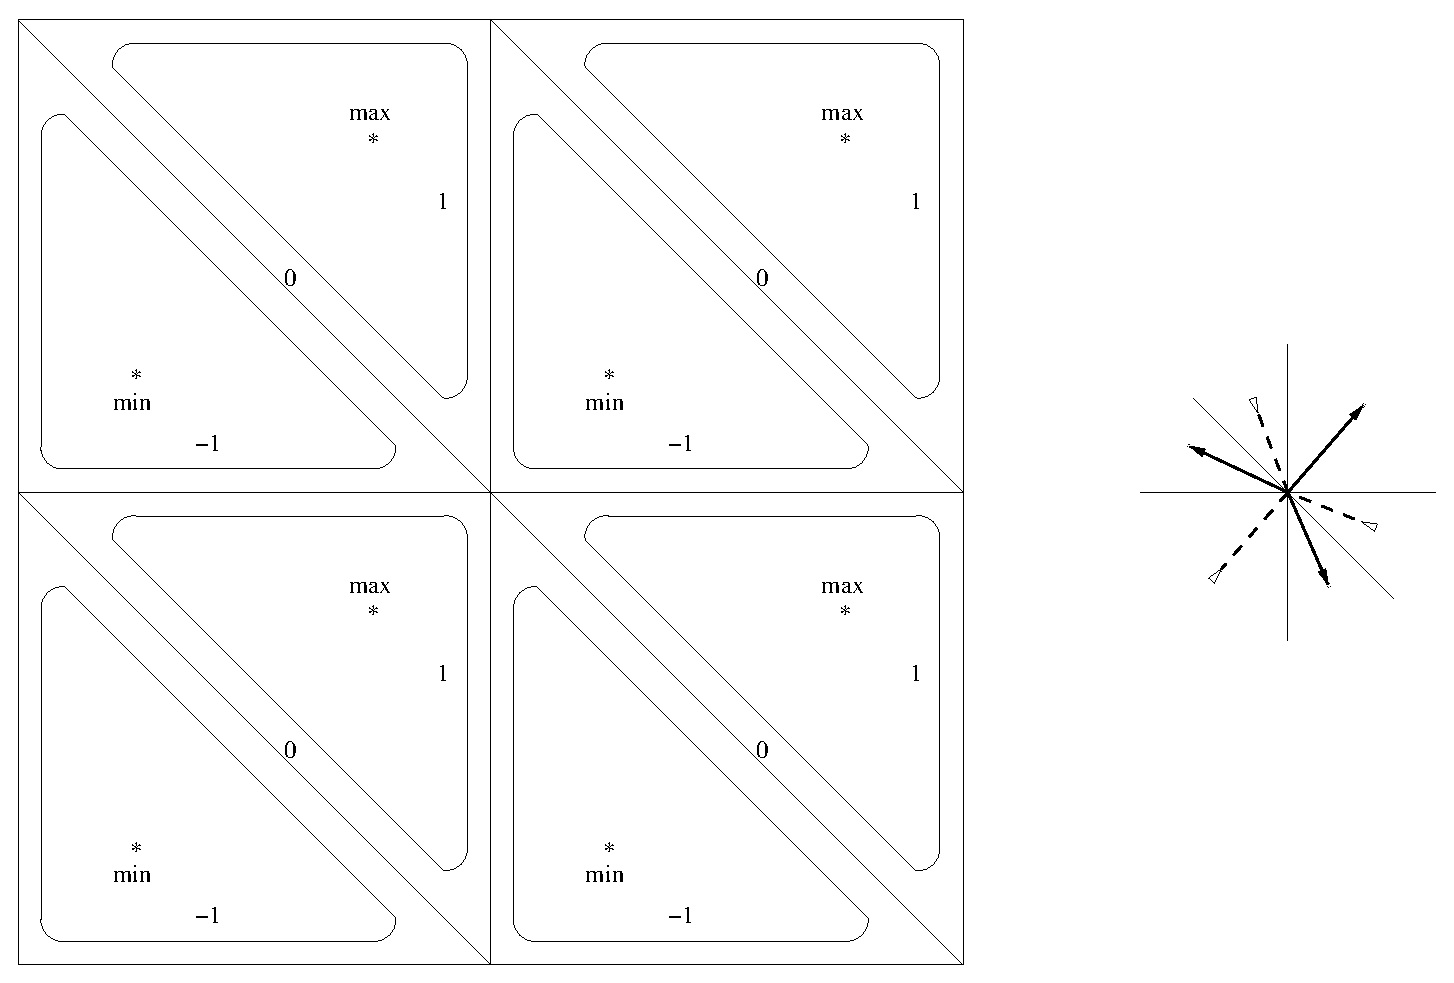
\includegraphics[scale=.5]{fig/14.13a.eps}
 \caption*{Figure 14.14 in four copies (left), and a zoom in on the central point}
\end{figure}

%%%%%%%%%%%%%%%%%%%%%%%%%%%%%%%%%%%%%%%%%%%%%%%%%%%%%%%%%%%%%%%%%%

\problem{14.3(5)} Let us consider
\[\begin{aligned}
 \mathcal{M}(t) - P(t) &= \cdots + (m_{\lambda-1}-b_{\lambda-1})t^{\lambda-1} + (m_{\lambda}-b_\lambda)t^\lambda + (m_{\lambda+1}-b_{\lambda+1})t^{\lambda+1}+\dots\\
 &=-b_{\lambda-1}t^{\lambda-1} + (m_\lambda-b_\lambda)t^\lambda -b_{\lambda+1}t^{\lambda+1}+\dots\\
 &= \dots+(q_{\lambda-1}+q_{\lambda-2})t^{\lambda-1} + (q_\lambda+q_{\lambda-1})t^\lambda + (q_{\lambda+1}+q_\lambda)t^{\lambda+1}+\dots = (1+t)Q(t)\,,
\end{aligned}\]
where $Q(t)=\sum_\lambda q_\lambda t^\lambda$, with $q_\lambda \ge 0$. As all coefficients are non-negative in the last line, therefore $0 = b_{\lambda-1}=b_{\lambda+1}$ must hold, so
\[
 \begin{aligned}
  0 = m_{\lambda-1}-b_{\lambda-1} &= (q_{\lambda-1}+q_{\lambda-2})\ge 0\,,\\
  m_\lambda-b_\lambda &= (q_\lambda+q_{\lambda-1})\ge 0\,,\\
  0 = m_{\lambda+1}-b_{\lambda+1} &= (q_{\lambda+1}+q_{\lambda})\ge 0
 \end{aligned}
\]
must hold too. This is only possible if $q_{\lambda, \lambda\pm 1}=0$, yielding $m_\lambda=b_{\lambda}$.

%%%%%%%%%%%%%%%%%%%%%%%%%%%%%%%%%%%%%%%%%%%%%%%%%%%%%%%%%%%%%%%%%%

\section{Lie groups, bundles, and Chern forms}

\subsection{Lie groups}

%%%%%%%%%%%%%%%%%%%%%%%%%%%%%%%%%%%%%%%%%%%%%%%%%%%%%%%%%%%%%%%%%%

\problem{15.1(1)} The right-invariant field ${\bf X}$ and ${\bf Y}$ must satisfy ${\bf X}_e=\partial/\partial x$ and ${\bf Y}_e=\partial/\partial y$, and be right-invariant, that is $R_{g*} {\bf X}_h = {\bf X}_{hg}$ (and the same for ${\bf Y}$), or, similarly to the treatment of the left-invariant fields in the book, ${\bf X}_g = R_{g*}{\bf X}_e$. This, as for the left-invariant fields, is obtained by multiplying its matrix at the origin with the group element, but now from the right, so
\[
 {\bf X}_g = R_{g*}\frac{\partial}{\partial x} = \left.\frac{\d}{\d t}\begin{pmatrix} 1+ t & 0 \\ 0 & 1\end{pmatrix}
 \begin{pmatrix} x & y \\ 0 & 1\end{pmatrix}\right|_{t=0} = \begin{pmatrix} x & y \\ 0 & 0 \end{pmatrix} = x\frac{\partial}{\partial x}+y\frac{\partial x}{\partial y}\,,
\]
and similarly, ${\bf Y}_g = \partial/\partial_y$. The dual right invariant forms satisfy $\sigma^1({\bf X}) = 1$, $\sigma^1({\bf Y}) = 0$, $\sigma^2({\bf X}) = 0$ and $\sigma^2({\bf Y}) = 1$. This is satisfied by $\sigma^1 = \d x/x$ and $\sigma^2=-y\d x/x + \d y$. The right-invariant volume form is $\sigma^1\wedge \sigma^2=\d x\wedge \d y/x$.

%%%%%%%%%%%%%%%%%%%%%%%%%%%%%%%%%%%%%%%%%%%%%%%%%%%%%%%%%%%%%%%%%%

\problem{15.1(2)} (i) for any $g\in G$, $g$ is a function $g:\mathbb{R}^4\to \mathbb{R}^4$, $x\mapsto gx$ (the linear action). The differential maps a $T_x \mathbb{R}^4\equiv \mathbb{R}^4$ to $T_{gx}\mathbb{R}^4$. The mapping is constructed, e.g., as considering a curve $\gamma(t)$ derivative at $t=0$ is a given vector, $\gamma(0)=x$, $\dot\gamma(0)={\bf v}$, e.g., $\gamma(t) = x+{\bf v}t$. The image of the vector is $g_* {\bf v} = \d/\d t( g \gamma(t))|_{t=0} = g{\bf v}$, whose matrix is $g$, so $\det g_* = \det g = 1$. This shows that it preserves the eucludean volume form: let ${\bf T}_i$, $i=1, \dots, 4$ be left-invariant vector fields, so $(g^* {\rm vol}_{gx})({\bf T}_{1x}, \dots, {\bf T}_{4x}) = {\rm vol}_{gx}(g_*{\bf T}_{1x}, \dots, g_*{\bf T}_{4x}) = {\rm vol}_{gx}({\bf T}_{1gx},\dots, {\bf T}_{4gx})$. On one hand, the euclidean volume does not depend on the point where it is evaluated, ${\rm vol}_{gx} = {\rm vol}$. On the other, ${\rm vol}_{gx}(g_*{\bf T}_{1x}, \dots, g_*{\bf T}_{4x}) = (\det g){\rm vol}({\bf T}_{1x},\dots, {\bf T}_{4x}) = {\rm vol}({\bf T}_{1x},\dots, {\bf T}_{4x})$, which, compared with the first expression, yields $g^*{\rm vol} = {\rm vol}$.

(ii) The group is the manifold $\{x | \det x = 1\}$, so the tangent space is the $\d H =0$, where $\d H (h) = (\det x) \Tr(x^{-1} h)$, therefore
\[
 T_x {\rm Sl}(2, \mathbb{R}) = \{h\in \mathbb{R}^4| \Tr x^{-1}h =0 \}\,.
\]
Calculating the inverse of the matrix using Cramer's rule, and using $\det x =1$ yields
\[
 ( x^{-1} )^i = (-1)^{\frac{(i-1)(4-i)}{2}}x^i\,,
\]
and so the tangent space is
\[
 \sum_i (-1)^{\frac{(i-1)(4-i)}{2}}x^i \d x^i = 0\,,
\]
which may be used to express $x^4\d x^4 = -\sum_{i=1}^3 (-1)^{(i-1)(4-i)/2} x^i \d x^i$.

The differential of the determinant function is
\[
 \d H = (\det x)(x^{-1})^i \d x^i\,,
\]
therefore the gradient vector is
\[
 (\nabla H)^i = (\det x) \sum_i (-1)^{\frac{(i-1)(4-i)}{2}}x^i\,,\quad\quad \|\nabla H\|^2 = (\det x)^2 \|x\|^2\,.
\]
The euclidean volume form is ${\rm vol} = \d x^1\wedge \d x^2 \wedge \d x^3 \wedge \d x^4$, and we shall insert here the gradient vector,
\[
 \sigma = i_{\nabla H/\|\nabla H\|^2}{\rm vol}
\]
yielding
\[
 \sigma=\frac{x^1}{\|x\|^2} \d x^2 \wedge \d x^3 \wedge \d x^4 + \frac{x^2}{\|x\|^2}\d x^1 \wedge \d x^3 \wedge \d x^4 - \frac{x^3}{\|x\|^2} \d x^1 \wedge \d x^2 \wedge \d x^4 - \frac{x^4}{\|x\|^2}\d x^1 \wedge \d x^2 \wedge \d x^3
\]
and we may express now $\d x^4$ with the rest, and only the independent one contributes,
\[
 \sigma = \d x^1 \wedge \d x^2 \wedge \d x^3 \left( -\frac{(x^1)^2}{x^4\|x\|^2} - \frac{(x^2)^2}{x^4 \|x\|^2} -\frac{(x^3)^2}{x^4 \|x\|^2} - \frac{x^4}{\|x\|^2}\right) = -\frac{x^1}{1+x^2 x^3}\d x^1 \wedge \d x^2 \wedge \d x^3\,.
\]
We may, of course, flip the orientation.

%%%%%%%%%%%%%%%%%%%%%%%%%%%%%%%%%%%%%%%%%%%%%%%%%%%%%%%%%%%%%%%%%%

\problem{15.2(1)} Let us use the series of $\exp x$,
\[
 \exp \theta J = \sum_n \frac{1}{n!}(\theta J)^n\,,
\]
and replace $(\theta J)^n = \theta^n J^n$, and take into account $J^2=-I$, separate $n=2k$ and $n=2k+1$, yielding
\[
 \exp\theta J = \sum_k \frac{1}{(2k)!}(-1)^k \theta^{2k} I + \sum_k \frac{1}{(2k+1)!} (-1)^k \theta^{2k+1} J = (\cos\theta)I+(\sin\theta)J\,,
\]
where we have recognised the power series of the sine and cosine functions.

%%%%%%%%%%%%%%%%%%%%%%%%%%%%%%%%%%%%%%%%%%%%%%%%%%%%%%%%%%%%%%%%%%

\problem{15.2(2)} Let us first show (by induction) that
\[
 \begin{pmatrix} a & b \\ 0 & 0 \end{pmatrix}^n = \begin{pmatrix} a^n & a^{n-1} \\ 0 & 0 \end{pmatrix}
\]
for $n\ge 1$. Then
\[
 \exp t \begin{pmatrix} a & b \\ 0 & 0 \end{pmatrix} = I+\sum_{n=1}^\infty \frac{t^n}{n!} \begin{pmatrix} a^n & (a)^{n-1}b \\ 0 & 0 \end{pmatrix}\,,
 \]
and the sums are
\[
1+\sum_{n=1}^\infty (ta)^n/n! = \sum_{n=0}^\infty = \exp(ta)
\]
and
\[\sum_{n=1}^\infty t^n a^{n-1}b/n!= (b/a)\sum_{n=1}^\infty (ta)^n/n!= b/a(\exp(at)-1)
\]
 yielding
\[
 \exp t \begin{pmatrix} a & b \\ 0 & 0 \end{pmatrix} = \begin{pmatrix} \exp(at) & \frac{b}{a}(\exp(at)-1) \\ 0 & 1 \end{pmatrix}\,.
\]

%%%%%%%%%%%%%%%%%%%%%%%%%%%%%%%%%%%%%%%%%%%%%%%%%%%%%%%%%%%%%%%%%%

\problem{15.2(3)} The convergence radius of the series of the exponential is infinite, therefore, we may differentiate term by term.
\[
 \exp[B(t)] = \sum_n \frac{B(t)^n}{n!}\,,
\]
and $\d / \d t B(t)^n = B'(t) B(t)^{n-1} + B(t) B'(t) B(t)^{n-2}+\dots = n A(t) B(t)^{n-1}$, therefore
\[
 \frac{\d}{\d t}\exp[B(t)] = \sum_n \frac{1}{n!} n A(t) B(t)^{n-1} = A(t)\sum_n \frac{B(t)^{n-1}}{(n-1)!} = A(t)\exp[B(t)]\,,
\]
which completes the proof.

%%%%%%%%%%%%%%%%%%%%%%%%%%%%%%%%%%%%%%%%%%%%%%%%%%%%%%%%%%%%%%%%%%

\problem{15.3(1)} We start by choosing a set of left-invariant vector fields ${\bf X}_R$, $R=1, 2, \dots$, $\dim G$, defining the structure constants by $[{\bf X}_R, {\bf X}_S] = {\bf X}_T C^T_{RS}$. The dual basis of one-forms, defined by $\sigma^U({\bf X}_S)=\delta^U_S$ is also left-invariant, therefore, as in eq.\ (15.22),
\[
 \d\sigma^U ({\bf X}_R, {\bf X}_S)=-\sigma^U([{\bf X}_R, {\bf X}_S]) = -\sigma^U({\bf X}_T C^T_{RS}) = -C^U_{RS} = -\sum_{U<V}C^U_{UV}\sigma^U\wedge\sigma^V({\bf X}_R, {\bf X}_S)
\]
for any two basis vector fields ${\bf X}_R, {\bf X}_S$, therefore, the two forms must agree,
\[
 \d\sigma^U = -\sum_{R<S}C^U_{RS}\sigma^R\wedge\sigma^S = -\frac{1}{2}\sum_{R, S}C^U_{RS}\sigma^R\wedge\sigma^S\,.
\]

The Jacobi identity on the structure constants is proved as dollows: as $\d\d\sigma^U = 0$, so using eq.\ (4.27) yields
\[\begin{aligned}
 0 = \d(\d\sigma^U)({\bf X}_L, {\bf X}_M, {\bf X}_S) &= 
 {\bf X}_L(\d\sigma^U({\bf X}_M, {\bf X}_S)) -{\bf  X}_M (\d\sigma^U({\bf X}_L, {\bf X}_S)) + {\bf X}_S(\d\sigma^U({\bf X}_L, {\bf X}_M))\\
 &-\d\sigma^U([{\bf X}_L, {\bf X}_M], {\bf X}_S) + \d\sigma^U([{\bf X}_L,{\bf X}_S], {\bf X}_M) -\d\sigma^U([{\bf X}_M,{\bf X}_S], {\bf X}_L)\,,
\end{aligned}
\]
and the terms in the first row are 0 (as they are derivatives of the structure constants along the vectors). In the second row, we write $[{\bf X}_L, {\bf X}_S] = {\bf X}_T C^T_{RS}$, and so on,
yielding
\[
 C^U_{RS}C^R_{LM} + C^U_{RM}C^R_{SL} + C^U_{RL}C^R_{MS} = 0\,.
\]


%%%%%%%%%%%%%%%%%%%%%%%%%%%%%%%%%%%%%%%%%%%%%%%%%%%%%%%%%%%%%%%%%%

\problem{15.3(2)} As $A^2=-\rho I$, the series of the exponential can be separated into odd and even terms as
\[
 \e^A = \sum_{n=0}^\infty \frac{A^n}{n!} = \sum_{k=0}^\infty \frac{(-1)^k \rho^k}{(2k+1)!} A + \sum_{k=0}^\infty \frac{(-1)^k \rho^k}{(2k)!} I\,,
\]
where we may replace $\rho^k = (\sign \rho)^k \sqrt{\rho \sign \rho }^{2k}$, thereby obtaining the desired result.

As $A$ is zero trace,
\[
 \Tr \e^A = \left\{
 \begin{aligned}
  2\cos\sqrt\rho&\,,\quad\text{\ if $\rho > 0$}\\
  2\cosh\sqrt{|\rho|}&\,,\quad\text{\ if $\rho < 0$}\\
  2&\,,\quad\text{\ if $\rho = 0$}\\
 \end{aligned}
 \right.
\]
which also yields $\Tr \e^A \ge -2$. The matrix $g$ above has $\Tr g = -3/2$, therefore it cannot be of the form $\e^A$ for a traceless $A$.

%%%%%%%%%%%%%%%%%%%%%%%%%%%%%%%%%%%%%%%%%%%%%%%%%%%%%%%%%%%%%%%%%%

\problem{15.3(3)} (i) For any element $g\in {\rm Sl}(n, \mathbb{R})$ its columns ${\bf v}_1, \dots, {\bf v}_n\in \mathbb{R}^n$ are $n$ linearly independent numbers. Let us consider their Gram-Schmidt orthogonalisation ${\bf e}_1$, \dots, ${\bf e}_n$, and the vectors ${\bf w}_k = t {\bf e}_k + (1-t) {\bf v}_k$, which agree with ${\bf }_k$ for $t=0$, and with ${\bf e}_k$ for $t=1$. This shows that ${\rm SO}(n)$ is a deformation retract of ${\rm Sl}(n, \mathbb{R})$. As the latter is connected [see Theorem (15.5)], so is the former.

(ii) As the group is a deformation retract of ${\rm SO}(3)$, their homology groups agree. The latter is a ball in the space if $3\times 3$ real matrices with the opposite points on its boundary identified, i.e, the real projective space $\mathbb{R}P^3$. That has (see Sec.\ 13.3b) $H_0({\rm Sl}(3, \mathbb{R}), \mathbb{R})=\mathbb{R} = H_3({\rm Sl}(3, \mathbb{R}), \mathbb{R})$, and all others 0, and from Problem 13.3(1),  $H_0({\rm Sl}(3, \mathbb{Z}), \mathbb{R})=\mathbb{Z}$, $H_1({\rm Sl}(3, \mathbb{Z}), \mathbb{R})=\mathbb{Z}/2\mathbb{Z}=\mathbb{Z}_2$, $H_2({\rm Sl}(3, \mathbb{Z}), \mathbb{R})=0$ and $H_3({\rm Sl}(3, \mathbb{Z}), \mathbb{R})=\mathbb{Z}$ and all others 0.

(iii) The general linear group contains all matrices with a non-zero determinant. As the determinant is a polynomial, therefore, a continuous function of the matrix, the pre-image of a non-connected set $\mathbb{R}^+ \cup \mathbb{R}^-$ cannot be connected.  At the same time, for all matrices $M\in {\rm Gl}(n, \mathbb{R})$ we may introduce $M(t) = (1-t) M + t M/\sqrt[n]{|\det M|}$ which connects it with $M(1)$ having $\det M(1) = \pm 1$. %Thus ${\rm Gl}(n, \mathbb{R})$ is a pre-image of $\{\pm 1\} {\rm Sl}(n, \mathbb{R})$ by a continuous function, and the latter is non-connected, therefore, so is ${\rm Gl}(n, \mathbb{R})$.
This shows that ${\rm Gl}(n, \mathbb{R})$ has a deformation retract $\{\pm 1\}{\rm Sl}(n, \mathbb{R})$, and so $\{\pm 1\}{\rm SO}(n) = {\rm O}(n)$. As a result, ist homology groups are the direct sum of those of ${\rm O}(n)$ with themselves.

%%%%%%%%%%%%%%%%%%%%%%%%%%%%%%%%%%%%%%%%%%%%%%%%%%%%%%%%%%%%%%%%%%

\problem{15.4(1)} We use eq.\ (15.33),
\[
 [{\bf X}, {\bf Y}] = \lim_{t\to 0}\frac{\exp(t{\bf X})\exp(t{\bf Y})\exp(-t{\bf X})\exp(-t{\bf Y})-I}{t^2}\,,
\]
and (15.17), $\exp S = \sum_n S^n/{n!}$. We expand all exponentials to second order, yielding
\[
\begin{aligned}{}
 [{\bf X}, {\bf Y}] &= \lim_{t\to 0}\frac{\left(I+tX+\frac{t^2 X^2}{2}\right) \left(I+tY+\frac{t^2 Y^2}{2}\right) \left(I-tX+\frac{t^2 X^2}{2}\right) \left(I- tY+\frac{t^2 Y^2}{2}\right) - I}{t^2}\\
 &= X Y-Y X\,.
\end{aligned}
\]

%%%%%%%%%%%%%%%%%%%%%%%%%%%%%%%%%%%%%%%%%%%%%%%%%%%%%%%%%%%%%%%%%%

\problem{15.4(2)} Let $h$ in the leaf $H$. Again, by the definition of $\Delta$, left translation of $H$ by $h^{-1}$ sends the lead into another, perhaps different, leaf $h^{-1} H$. On the other hand, $h\in H$ and so $e = h^{-1} h \in h^{-1} H$, i.e., the two leaves both contain $e$, therefore, they must coincide.

%%%%%%%%%%%%%%%%%%%%%%%%%%%%%%%%%%%%%%%%%%%%%%%%%%%%%%%%%%%%%%%%%%

\problem{15.4(3)} To show that it is a subalgebra, consider
\[
\begin{aligned}{}
 [A, B]^\dagger &= (AB-BA)^\dagger = B^\dagger A^\dagger - A^\dagger B^\dagger = (-B)(-A)-(-A)(-B)\\
 &= BA-AB = -(AB-BA) = -[A, B]\,,
\end{aligned}
\]
i.e., it is skew Hermitean, and
\[
 \Tr [A, B] = \Tr(AB-BA) = \Tr(AB) - \Tr(BA) = 0\,,
\]
as the trace is invariant to cyclic permutations. In Sec.\ 15.3c, it was shown that $\mathcal{su}(n)$, the Lie-algebra of ${\rm SU}(n)$ is the set of all skew Hermitean matrices.

In the case of Hermitean matrices, similar calculation yields
\[
 [A, B]^\dagger = (AB-BA)^\dagger = B^\dagger A^\dagger - A^\dagger B^\dagger = -(AB-BA) = -[A, B]\,,
\]
i.e., that the anticommutator is a skew Hermitean matrix, so their set does not form a Lie-algebra, therefore, there is no subgroup of ${\rm Sl}(n, \mathbb{C})$ whose Lie-algebra is the space of Hermitean matrices.


%%%%%%%%%%%%%%%%%%%%%%%%%%%%%%%%%%%%%%%%%%%%%%%%%%%%%%%%%%%%%%%%%%

\subsection{Vector bundles in geometry and physics}


%%%%%%%%%%%%%%%%%%%%%%%%%%%%%%%%%%%%%%%%%%%%%%%%%%%%%%%%%%%%%%%%%%

\problem{16.1(1)} It can be defined in one local trivialisation. What needs to be shown is that this is global: if $\psi^U = 0$
\[
 \psi^V(p) = c_{VU}(p) \psi_U(p) = 0\,,
\]
as the transition is linear.

%%%%%%%%%%%%%%%%%%%%%%%%%%%%%%%%%%%%%%%%%%%%%%%%%%%%%%%%%%%%%%%%%%

\problem{16.1(2)} If the bundle was trivial, one could specify a transportation of a frame ${\bf e}_{1,2}(p)$ in the normal bundle along the curve. As the tangent vector of the curve is ${\bf e}_3$, constant, there is a two-component matrix function $M(t)$ such that ${\bf e}(p(t)) = {\bf e}(p(0)) M(t)$.

The frame ${\bf e}_0 M(1)$ at the north pole is identified with $-{\bf e}_0 M(1)$ at the south pole, only possible if $\det M(1)=-1$. A continuous deformation is allowed (as in the proof of the triviality of the normal bundle of a closed curve in Euclidean 3-space in the book), but the determinant of an orthonormal matrix is either + or -1, so it cannot change continuously. This is a contradiction, so the bundle is non-trivial.

%%%%%%%%%%%%%%%%%%%%%%%%%%%%%%%%%%%%%%%%%%%%%%%%%%%%%%%%%%%%%%%%%%

\problem{16.1(3)} The normal bundle is a one-dimensional line bundle. If we take a line connecting two antipodal points, choose a vector at one point, it is identified with the opposite one at the antipodal point. Its single component therefore must vanish somewhere, therefore, the bundle is non-trivial, as there is not a single non-zero global section.

%%%%%%%%%%%%%%%%%%%%%%%%%%%%%%%%%%%%%%%%%%%%%%%%%%%%%%%%%%%%%%%%%%

\problem{16.1(4)} In the orientable case, the same argument may be used as in $\mathbb{R}^3$, transporting a frame along the curve, and if necessary, continuously deforming it in the last short part to match the original frame at 0 parameter value. This is possible as the frame together with the tangent vector specifies an orientation, and that must be the same as the one at 0 parameter value, therefore, the transported vectors are related to the original ones with an orientation-preserving transformation. Therefore, the normal bundle in this case is trivial.

In the non-orientable case, if $M$ is such a curve that an orientation cannot be transported along the curve, then assuming the existence of such a frame would result in the transportation of an orientation (as the tangent vector is preserved), resulting in a contradiction. Therefore, in this case, the normal bundle is not trivial.

%%%%%%%%%%%%%%%%%%%%%%%%%%%%%%%%%%%%%%%%%%%%%%%%%%%%%%%%%%%%%%%%%%

\problem{16.2(1)} The height vector field has one minimum at the point where the surface touches the table, one maximum at the top, and $2g$ saddle points. Around the maximum and the minimum, the surface is can be parametrised locally as $z=\pm(x^2+y^2)$, therefore vector field locally looks like the vector field $2{\bf x}$ and $-2{\bf x}$ on $\mathbb{R}^2$ near the origin, therefore its index at both these points is $1$. At the saddle points, the surface locally looks like the $z=\pm(x^2-y^2)$, therefore the vector field locally looks like $\pm(2x, -2y)$, which has index -1, therefore, adding the indices together, the desired result is proven.

%%%%%%%%%%%%%%%%%%%%%%%%%%%%%%%%%%%%%%%%%%%%%%%%%%%%%%%%%%%%%%%%%%

\problem{16.2(2)} The index of the critical points is 0, 1, and 2, in the order as above. The Morse indices are $m_0 = m$, $m_1=s$, and $m_2=M$, where $m$, $s$, and $M$ are the numbers of local minima, saddle points, and local maxima.

The pits-passes+peaks theorem yields (by using a triangulation fitted to the function) that there is a vertex for each maximum, a saddle point for each edge, and a face for each minimum, yielding $\chi = b_0 - b_1 + b_2$.

As the index of the vector field is $m - s + M = m_0 - m_1 + m_2$, and this must agree with $\chi$, we have proven Morse's equality.

%%%%%%%%%%%%%%%%%%%%%%%%%%%%%%%%%%%%%%%%%%%%%%%%%%%%%%%%%%%%%%%%%%

\problem{16.3(1)} First, let us note that from the definition,
\[
 \boldsymbol\nabla''_{\bf X}({\bf e}_a\otimes {\bf e}'_R) = (\boldsymbol\nabla_{\bf X}{\bf e}_a)\otimes {\bf e}'_R + {\bf e}_a\otimes (\boldsymbol\nabla'_{\bf X}{\bf e}'_R) = ({\bf e}_b \omega^b{}_a({\bf X}))\otimes {\bf e}'_{R} + {\bf e}_a \otimes ({\bf e}_S \omega'{}^S{}_R({\bf X}))
\]
on one hand, and on the other
\[
 \boldsymbol\nabla''_{\bf X} ({\bf e}_a\otimes{\bf e}'_R) = {\bf e}_b\otimes{\bf e}'_S \omega''{}^{bS}{}_{aR}({\bf X})\,,
\]
yielding
\[
 \omega''{}^{bS}{}_{aR} = \omega^b{}_a \delta^S_R + \delta^b_a \omega'{}^S{}_R\,,\quad \omega''{}^{ibS}{}_{aR} = \omega^b{}_{ia} \delta^S_R + \delta^b_a \omega'{}^S{}_{iR}\,.
\]

By definition,
\[
 \boldsymbol\nabla''_{\bf X}\boldsymbol\Lambda = ({\bf e}_a\otimes {\bf e}'_R) X^j\left(\partial_j \lambda^{aR} + \omega''{}^{aR}{}_{bS}\lambda^{bS}\right) = {\bf e}_a\otimes{\bf e}'_R X^j \nabla_j\lambda^{aR}
 %(\partial_j \lambda^{aR}+\omega''{}^{aR}{}_{bS}\lambda^{bS})
\]
yielding
\[
 \nabla_j\lambda^{aR} = \partial_j \lambda^{aR} + \omega''{}^{aR}{}_{jbS}\lambda^{bS} = \partial_j \lambda^{aS} + \omega^a_{jb}\lambda^{bR} + \omega'{}^R{}_{jS}\lambda^{aS}\,.
\]

%%%%%%%%%%%%%%%%%%%%%%%%%%%%%%%%%%%%%%%%%%%%%%%%%%%%%%%%%%%%%%%%%%

\problem{16.4(1)} Let us use Maxwell's equations,
\[
 \frac{\d}{\d t}\int_z \mathcal{B}^2 = \int_z \frac{\partial}{\partial t}\mathcal{B} = -\int_z {\bf d}\mathcal{E}^1 = -\int_{\partial z}\mathcal{E} =0\,,
\]
as $z$ is a cosed surface, $\partial z=\emptyset$.

%%%%%%%%%%%%%%%%%%%%%%%%%%%%%%%%%%%%%%%%%%%%%%%%%%%%%%%%%%%%%%%%%%

\problem{16.4(2)} The difference between the two local sections in the overlap region $U\cap V$ is
\[
 \mathcal{A}^1_V - \mathcal{A}^1_U = -2q\d\varphi\,,
\]
and this multiplied by $-\imagi e/\hbar$ shall agree with
\[
 -c_{VU}^{-1} \d c_{VU} = -\exp\left(\frac{2\imagi eq\varphi}{\hbar}\right)\d \exp\left(-\frac{2\imagi eq\varphi}{\hbar}\right)  = \frac{2\imagi e q}{\hbar}\d\varphi\,,
\]
which holds.

%%%%%%%%%%%%%%%%%%%%%%%%%%%%%%%%%%%%%%%%%%%%%%%%%%%%%%%%%%%%%%%%%%

\problem{16.4(3)} Let us consider the extension using the transition formula (16.47), with the transition function (16.51)
\[
 \psi_V(x) = c_{VU}(x)\psi_U(x) = \exp\left(-\frac{2\imagi e q\varphi}{\hbar}\right)\,,
\]
and examine this $\psi_V$ around the negative $z$ axis, where its value us discontinuous. This shows that $\psi_V$ cannot be the coordinate form of a smooth section of the bundle there, therefore $\psi_U$ cannot be extended to the whole space outside the origin.

%%%%%%%%%%%%%%%%%%%%%%%%%%%%%%%%%%%%%%%%%%%%%%%%%%%%%%%%%%%%%%%%%%

\problem{16.4(4)} Transforming to cylindrical coordinates is $x=r\cos\vartheta$, $y=r\sin\vartheta$, so $\d x = \cos\vartheta \d r-r\sin\vartheta \d\vartheta$, $\d y = \sin\vartheta \d r + r\cos\vartheta\d\vartheta$, so $\mathcal{B} = B \d x \wedge \d y = B r \d r \wedge \d\vartheta$. [The same result could be reached by noting that $\d x \wedge \d y = r \d r\wedge \d\vartheta$ is the area (2d volume) form of the plane $xy$.] This is compared with $\d \mathcal{A} = \d [(B/2) r^2 \d\vartheta] = B r \d r \wedge\d\vartheta$.

The vector corresponding to the potential form is obtained with the inverse metric, as $g_{rr} = 1$, $g_{\vartheta\vartheta}=r^2$, $g_{zz}=1$ (all other components vanish), $g^{rr}=1$, $g^{\vartheta\vartheta}=r^{-2}$, $g^{zz}=1$, yielding ${\bf A} = (B/2) \partial_\vartheta$, and $\|{\bf A}\|^2=A^\vartheta \mathcal{A}_\vartheta  = B^2 r^2/4 = b^2r^2/(4\pi^2 a^4)$. For the exterior potential, $\mathcal{A}_{\rm exterior} = b \d\vartheta/(2\pi)$, the norm is $\|{\bf A}_{\rm exterior}\|^2 = b^2/(4\pi^2 r^2)$.

At $r=a$, the two do match, for the inner field, $\|{\bf A}\|^2|_{r=a} = b^2/(4\pi^2 a^2)$ and for the exterior one, $\|{\bf A}_{\rm exterior}\|^2|_{r=a}=b^2/(4\pi^2)$, but not smoothly, the interior one is growing quadratically and the exterior one falling off as $1/r^2$, the derivative jumps. This is because the iterior has a constant magnetic field $B$, and the outside magnetic field vanishes. At $r=a$ is the coil, with a current flowing in it.

%%%%%%%%%%%%%%%%%%%%%%%%%%%%%%%%%%%%%%%%%%%%%%%%%%%%%%%%%%%%%%%%%%

\problem{16.4(5)} On one hand, direct transformation yields
$c_{VU}(y, t)$ times the above result, as it is a contribution of this path to $\psi_V(y, t)$. On the other hand, using the formula in the patch $V$ yields
\[
 \psi_V(x, 0)\exp\left[\frac{\imagi}{\hbar}\int_\gamma L\d t\right] \exp\int_\gamma(-\omega_V)\,.
\]
Here $\psi_V(x, 0)=c_{VU}(x, 0) \psi_{U}(x, 0)$ and $\omega_V = \omega_U + \d\log c_{UV} = \omega_U -\d\log c_{VU}$, so
\[
 \exp\int_\gamma (-\omega_V) = \exp\left[\int_\gamma (-\omega_U) +\log c_{VU}(y, t) - \log c_{VU}(x, 0)\right]
\]
therefore the two expressions agree, and gauge invariance is proven.
%%%%%%%%%%%%%%%%%%%%%%%%%%%%%%%%%%%%%%%%%%%%%%%%%%%%%%%%%%%%%%%%%%

\subsection{Fiber bundles, Gauss-Bonnet, and topological quantisation}

%\subsubsection{Fiber bundles and principal bundles}


%%%%%%%%%%%%%%%%%%%%%%%%%%%%%%%%%%%%%%%%%%%%%%%%%%%%%%%%%%%%%%%%%%

\problem{17.2(1)} Let us note that the projective space $\mathbb{R}P^{n-1}$ is the set of unoriented lines (i.e., 1-planes) in $\mathbb{R}^n$, $\mathbb{R}P^{n-1} = {\rm Gr}(n-1, n)$. We may thus follow the construction of sec.\ 17.2b.  The orthogonal group ${\rm O}(n)$ acts naturally on $\mathbb{R}^n$. The subgroup that sends a given space into itself acts as ${\rm O}(n-k)$ on the orthogonal complement of a $k$ dimensional subspace, and in the $k$-dimensional subspace $O(1)=\{\pm 1\}$ flips the orientation, therefore
\[
 {\rm Gr}(k, n) \cong \frac{{\rm O}(n)}{{\rm O}(1)\times {\rm O}(n-k)}\,.
\]

The dimension is therefore that of ${\rm O}(n)$ minus that of ${\rm O}(n-k)$, $n(n-1)/2 - (n-k)(n-k-1)/2 = k(2n-k-1)/2$.

%%%%%%%%%%%%%%%%%%%%%%%%%%%%%%%%%%%%%%%%%%%%%%%%%%%%%%%%%%%%%%%%%%

\problem{17.2(2)} The two curves were $C={\rm SO}(2)$, rotations around the $z$ axis (leaving the $z$ axis invariant), and $C'$ the coset of the rotation ${\rm diag}(1, -1, -1)$.

We construct a mapping from ${\rm SO}(3)$ to $\mathbb{R}P^2$ as follows. To any group element (rotation) $g$ we assign the line that correspond to $g n$, where $n$ is the north pole. In this way, the projective space is the factor space ${\rm SO}(3)/H$, where $H$ is the group leaving a point in the projective space invariant. We shall show that this is the subgroup generated by $C\cup C'$.

Factoring the group ${\rm SO}(n)$ by the curve $C$ yields a sphere $S^2$, as shown in the text: any point on $S^2$ may be written as obtained from the north pole by a rotation, and rotations leaving the point $p$ invariant may be written as $ghg^{-1} g$ where $gn =p$, $n$ is the north pole, and $hn=n$, i.e., $h\in C$.

Consider a point $p\in S^2$, and $x\in S^2$ beint the point of $S^2$ on the positive $x$ axis. For both of these, there exist group elements in ${\rm SO}(3)$ such that $g_p n = g$, $g_x n=x$. Let $c = {\rm diag}(1,-1,1)$, then $g_p g_x^{-1}cg_xg_p^{-1} = g_p g_x^{-1}c g_x n = g_p g_x^{-1} c x = -g_p g_x^{-1}x = -g_p n = -p$, so factorising with $C'$ identifies antipodal points in $S^2$.

%%%%%%%%%%%%%%%%%%%%%%%%%%%%%%%%%%%%%%%%%%%%%%%%%%%%%%%%%%%%%%%%%%

\problem{17.2(3)} Any $k$-frame can be extended by adding $n-k$ vectors into an $n$-frame. The space of $n$-frames can be identified with $O(n)$. The extension is ambiguous, as any orthogonal transformation that leaves the original $k$ vectors invariant can be applied on the additional vectors.

$S^{n-1}$ is therefore the $k=1$ case, $S^{n-1}\cong {\rm O}(n)/{\rm O}(n-k)$. In the text $S^{n-1}\cong {\rm SO}(n)/{\rm SO}(n-k)$ was shown. An orientation flipping transformation, in this sense, ``can be cancelled''. The same holds for the Stiefel manifolds for $k<n$, but not for $k=n$.

%%%%%%%%%%%%%%%%%%%%%%%%%%%%%%%%%%%%%%%%%%%%%%%%%%%%%%%%%%%%%%%%%%

\problem{17.4(1)} The transition function for the two coordinate patches for the manifold is constructed in sec.\ 1.2d.\ in the book, yielding $w=f_{wz}(z) = 1/z$. The transition function $c_{wz}$ is a mapping between coordinates of vectors in the two patches. Note, that a coordinatisation (inverse of a chart) in a patch is a mapping $p_z: \mathbb{C}\to S^2$, and a vector in the tangent space may be coordinatised by pushing a vector forward by $p_{z*}$, so $c_{wz} = (p_{w*})^{-1} p_z = (p_w^{-1} \circ p_z)_*$. If $w=f_{wz}(z)=p_w^{-1}(p_z(z)) = 1/z$, i.e., $f_{wz}=p_w^{-1}\circ p_z$, we get $c_{wz}= f_{wz*}$, $(c_{wz*})_z(\zeta) = -1/z^2 \zeta$.


A tangent vector may be coordinatised by $\phi_u$, as follows: $\phi_z {\bf v} = (p_z^{-1})_* {\bf v}$ and $\phi_v {\bf v} = (p_w^{-1})_* {\bf v}$. 

Using the construction in sec.\ 1.2d, we get for the point on $S^2\subset \mathbb{R}^2$, $p_z(z) = (x, y, (1-x^2-y^2)/2)^T/(1+x^2+y^2)$ where $z=x+\imagi y$, and similarly $p_w(w) = (u, v, (u^2+v^2-1)/2)^T/(1+u^2+v^2)$.

The tangent vectors are obtained as a derivative of the parametrisation, ${\bf v} = \partial_x p_z(z) \xi + \partial_y p_z(z) \eta$ where $\phi_z = \zeta = \xi + \imagi \eta$ and ${\bf v} = \partial_u p_w(w) \kappa + \partial_v p_w(w) \lambda$ where $\phi_w =\mu = \kappa + i \lambda$ and $\mu = c_{wz}(z) \zeta$.

The calculation yields $|{\bf v}|^2 = |\phi_z|^2/(1+|z|^2)^2 = |\phi_w|^2/(1+|w|^2)^2$. Substituting $\mu = -\xi/z^2$ and $w=1/z$ yields $|\phi_z|^2 |z^{-2}| = |\phi_w|^2 |w|^{-2} = |{\bf v}|^2(|z| + |z|^{-1})^2 = |{\bf v}|^2 (|w|^{-1} + |w|)^2$. This is the metric singular at the poles. At the same time, $(1+|z|^2)^{-2}|\phi_z|^2 = (1+|w|^2)^{-2} |\phi_w|^2 = |{\bf v}|^2$ is both independent of the patch used and non-singular.

%%%%%%%%%%%%%%%%%%%%%%%%%%%%%%%%%%%%%%%%%%%%%%%%%%%%%%%%%%%%%%%%%%

\problem{17.4(2)} According to eq.\ (17.30),
\[
 \omega = \langle {\bf e}(\alpha), \d {\bf e}(\alpha)\rangle = \left\langle {\bf e}, \frac{\partial\bf e}{\partial \alpha^k}\right\rangle \d\alpha^k\,.
\]
Choosing another basis $\e'(\alpha) = {\bf e}(\alpha)\e^{\imagi \beta(\alpha)}$ yields
\[
 \omega' = \langle {\bf e}'(\alpha), \d {\bf e}'(\alpha)\rangle = \left\langle {\bf e}\e^{\imagi\beta}, \d ({\bf e}\e^{\imagi\beta})\right\rangle = \left\langle {\bf e}\e^{\imagi\beta}, (\d{\bf e})\e^{\imagi\beta}+{\bf e}\e^{\imagi\beta}\imagi\,\d\beta\right\rangle =\omega + \imagi\,\d\beta\,, 
\]
which is the correct transformation rule.

%%%%%%%%%%%%%%%%%%%%%%%%%%%%%%%%%%%%%%%%%%%%%%%%%%%%%%%%%%%%%%%%%%

\problem{17.4(3)} We take the exterior derivative of $\theta$,
\[\begin{aligned}
 \d \left\langle {\bf e}, \frac{\partial {\bf e}}{\partial \alpha^k}\right\rangle\d\alpha^k &= \frac{\partial}{\partial \alpha^j}\left\langle {\bf e}, \frac{\partial {\bf e}}{\partial \alpha^k}\right\rangle\d\alpha^j\wedge\d\alpha^k\\
 &= \left\langle \frac{\partial{\bf e}}{\partial \alpha^j}, \frac{\partial {\bf e}}{\partial \alpha^k}\right\rangle\d\alpha^j\wedge\d\alpha^k + \left\langle {\bf e}, \frac{\partial^2 {\bf e}}{\partial\alpha^j\partial \alpha^k}\right\rangle\d\alpha^j\wedge\d\alpha^k\\
 &= \imagi \Im \left\langle \frac{\partial{\bf e}}{\partial \alpha^j}, \frac{\partial {\bf e}}{\partial \alpha^k}\right\rangle\d\alpha^j\wedge\d\alpha^k\,,
\end{aligned}\]
where in the second line, the second term vanishes due to the symmetry of partial derivatives and antisymmetry of the wedge product. As the wedge product is antisymmetric, in the same line, the scalar product may be antisymmetrised, and $\langle a, b \rangle - \langle b, a\rangle = \langle a, b \rangle - \overline{\langle a, b\rangle} = 2\imagi \Im \langle a, b\rangle$.

%%%%%%%%%%%%%%%%%%%%%%%%%%%%%%%%%%%%%%%%%%%%%%%%%%%%%%%%%%%%%%%%%%

\problem{17.4(4)} The covariant derivative of $\e^{\imagi \gamma(\alpha)}\phi_\alpha$ is
\[
 \nabla \phi\e^{\imagi\gamma} = (\nabla\phi)\e^{\imagi \gamma}+\phi \e^{\imagi\gamma}\imagi\,\d\gamma = \phi(\omega + \imagi\,\d\gamma)\e^{\imagi\gamma}\,,
\]
and along the curve $C$, according to eq.\ (17.33) $\d\gamma=\imagi\,\omega$, therefore $\imagi\d\gamma = -\imagi \omega$, so the covariant derivative vanishes along the curve.

%%%%%%%%%%%%%%%%%%%%%%%%%%%%%%%%%%%%%%%%%%%%%%%%%%%%%%%%%%%%%%%%%%

\problem{17.4(5)} Let us introduce polar coordinates, $z = r\e^{\imagi\varphi}$, so
\[
 \d z = \e^{\imagi\varphi}\d r + \imagi r \e^{\imagi \phi}\d\varphi\,.
\]
The basis section is
\[
 {\bf e}_U(z) = \frac{(1,r\e^{\imagi \varphi})^T}{(1+r^2)^{1/2}}\,.
\]
This yields
\[
 \d{\bf e}_U = \frac{(0, \d r \e^{\imagi\varphi}+\imagi r \e^{\imagi \varphi}\d\varphi)}{(1+r^2)^{1/2}} - \frac{(1, r\e^{\imagi \varphi})^T}{(1+r^2)^{3/2}}r\d r\,,
\]
and so
\[
 \omega_U = \langle {\bf e}_U, \d{\bf e}_U \rangle = \frac{\imagi r^2\d\varphi}{1+r^2}\,,
\]
which is eq.\ (17.38). Taking the exterior derivative yields
\[
 \d\omega_U = \imagi\,\d\frac{r^2}{1+r^2}\wedge\d\varphi = \frac{2\imagi\,r\d r\wedge\d\varphi}{(1+r^2)^2}\,,
\]
which is eq.\ (17.39). The integral is
\[
 \iint_S \frac{\imagi \theta}{2\pi} = -\frac{1}{\pi}\iint_S \frac{r\d r \d\varphi}{(1+r^2)^2} =- 2\int_0^\infty \frac{r\d r}{(1+r^2)^2} =- \int_0^\infty \frac{\d u}{(1+u)^2} = -\left[ \frac{u}{1+u}\right]_0^\infty = -1\,.
\]

%%%%%%%%%%%%%%%%%%%%%%%%%%%%%%%%%%%%%%%%%%%%%%%%%%%%%%%%%%%%%%%%%%

\subsection{Connections and associated bundles}

%%%%%%%%%%%%%%%%%%%%%%%%%%%%%%%%%%%%%%%%%%%%%%%%%%%%%%%%%%%%%%%%%%

\problem{18.1(1)} An element of the group is of the form
\[
 {\rm A}(1) \ni g=\begin{pmatrix}x & y \\ 0 & 1 \end{pmatrix}\,,
\]
therefore
\[
 g^{-1}\d g = \begin{pmatrix} 1/x & -y/x \\ 0 & 1 \end{pmatrix} \begin{pmatrix} \d x & \d y \\ 0 & 0 \end{pmatrix} = \begin{pmatrix} \frac{\d x}{x} & \frac{\d y}{x} \\ 0 & 0 \end{pmatrix}\,,
\]
and similarly
\[
 \d g g^{-1} = 
 \begin{pmatrix}
  \frac{\d x}{x} & \d y -\frac{y\d x}{x} \\
  0 & 0
 \end{pmatrix}\,.
\]

%%%%%%%%%%%%%%%%%%%%%%%%%%%%%%%%%%%%%%%%%%%%%%%%%%%%%%%%%%%%%%%%%%

\problem{18.1(2)} The connection form has the property
\[
 \nabla {\bf e}_U = {\bf e}_U \otimes \omega_U\,,\quad \nabla {\bf e}_V = {\bf e}_V \otimes \omega_V\,.
\]
The connection form therefore tranforms as
\[
 \omega_V = c_{UV}^{-1}\omega_U c_{UV} + c_{UV}^{-1}\d c_{UV}\,,
\]
and
\[
 \omega^*_U = g_U^{-1}\pi^* \omega_U g_U + g_U^{-1}\d g_U\,,
\]
and
\[
 \omega^*_V = g_V^{-1}\pi^* \omega_V g_V + g_V^{-1}\d g_V\,.
\]
Using the expression given in the problem for a point in the fiber, we obtain ${\bf f} = {\bf e}_V g_V = {\bf e}_U c_{UV} g_V = {\bf e}_U g_U$ yielding $g_V = c_{UV}^{-1}g_U$, so
\[
 \omega^*_V = g_U^{-1}c_{UV} \pi^* \omega_V c_{UV}^{-1} g_U + g_U^{-1}c_{UV} c_{UV}^{-1}\d g_U - g_U^{-1} c_{UV} c_{UV}^{-1} \d c_{UV} c_{UV}^{-1} g_U\,,
\]
where we used $c_{UV}^{-1}c_{UV}=e$, therefore $\d c_{UV}^{-1} c_{UV} + c_{UV}^{-1}\d c_{UV} = 0$.  We substitute $\omega_V$,  yielding
\[
 \omega_V^* =  g_U^{-1} \pi^* \omega_U g_U + g_U^{-1} \d c_{UV} c_{UV}^{-1}g_U + g_U^{-1}\d g_U - g_U^{-1} \d c_{UV} c_{UV}^{-1}g_U = \omega_U^*\,.
\]

%%%%%%%%%%%%%%%%%%%%%%%%%%%%%%%%%%%%%%%%%%%%%%%%%%%%%%%%%%%%%%%%%%

\problem{18.2(1)} (i) Consider a globally defined $n$-form $\sigma$. In any coordinate frame, we may write this as
\[
 \sigma = \sigma_{12\dots n}\d x^1\wedge\dots\wedge\d x^n\,,
\]
and on an overlap $U\cap V$, the transition function is obtained as follows,
\[
 \sigma_{V,i_1,\dots, i_n} = \frac{\partial x_U^{j_1}}{\partial x_V^{j_1}}\dots \frac{\partial x_U^{j_n}}{\partial x_V^{j_n}}\sigma_{U,j_1,\dots,j_n} = \det \frac{\partial x_U}{\partial x_V}\sigma_{U,i_1,\dots,i_n}\,,
\]
i.e., it satisfies the transformation rule of a section of the determinant bundle.

(ii) In an associated bundle with representation $\rho$, the connection form $\Omega$ is constructed, according to eq.\ (18.24) as $\Omega_U = \rho_* \omega$. What we need to obtain is the representation $\rho$, which, in the case of the determinant bundle is obtained as follows. In the tangent bundle, the transition functions are $c^t_{VU} = \partial x_V/x_U$, so $c_{VU} = \det (c^t_{VU})^{-1} = 1/\det c^t_{VU}$. Therefore
\[
 \Omega = \rho_*(\omega) = (1/\det)_* \omega = -\Tr\omega\,,
\]
as the derivative of the determinant at the unit is the trace, and the tangent to $1/\det$ is $(1/\det)_* = (-1/\det^2)\det_* = -\Tr$ as $\det e=1$.

(iii) In the case of a Riemannian manifold, the structure group is ${\rm O}(n)$, which has two disconnected components, therefore the determinant cannot change sign in one connected overlap of two patches. Let $U\cap V$ be a(connected component) of an overlap, and $\varepsilon$ the sign here, in any case, let $\Omega_U = -\Tr \omega_U$ and $\Omega_V = -\Tr\omega_V$. We know that $\omega_V = (c_{VU}^t)^{-1} \omega_U$.

Let us consider a section $\phi$ of the volume bundle that has its support within $U\cap V$. We shall suppress the indices $1,2,\dots, n$ on the components of the pseudoforms, simply writing the single component without indices. This transforms as $\phi_V = |\det c_{UV}^t| \phi_U $, therefore $\varepsilon \phi_U = \det c_{VU}^t \phi_U$, i.e., these define a section of the determinant bundle, where $\Omega_U = -\Tr\omega_U$ and $\Omega_V = -\Tr \omega_V$ yield a correct connection form, and the covariant derivative transforms as follows
\[
\begin{aligned}
 \nabla_{U\bf X} \phi_U &= {\bf X}(\phi_U) - \Tr\omega_U({\bf X}) \phi_U\,,\\
 \nabla_{V\bf X}\varepsilon\phi_V  &= {\bf X}(\varepsilon \phi_V) -\Tr\omega_V({\bf X})\varepsilon\phi_V = c_{VU}\nabla_{U\bf X}\phi_U
\end{aligned}
\]
This just yields the correct transformation law
\[
 \nabla_{V\bf X}\phi_V = \varepsilon c_{VU} \nabla_{U\bf X}\phi_U = c'_{VU} \nabla_{U\bf X}\phi_U\,.
\]

%%%%%%%%%%%%%%%%%%%%%%%%%%%%%%%%%%%%%%%%%%%%%%%%%%%%%%%%%%%%%%%%%%

\problem{18.2(2)} Let us consider the derivative of the representation at the unit element. The Lie algebra of ${\rm SO}(2)$ is the set of antisymmetric matrices, and the derivative of $\rho$ acts as follows,
\[
 \rho_*: \mathcal{g}\to \imagi \mathbb{R}\,,\quad
 \mathcal{g} \ni \begin{pmatrix} 0 & -1 \\ 1 & 0 \end{pmatrix} \mapsto \imagi\,,
\]
which can be seen by considering the inverse mapping an taking its ordinary derivative. The inverse mapping from ${\rm U}(1) \to {\rm SO}(2)$ is given by substituting $\theta = -\imagi \log \rho(g)$ into the parametrised form of the matrix.

Comparing the antisymmetric matrix
\[
 \begin{pmatrix} 0 & \omega_{12} \\ \omega_{21} & 0 \end{pmatrix}\,,\quad \omega_{12}=-\omega_{21}\,,
\]
and the above one, yields for the connection in the line bundle $\imagi \omega_{21}$, just as expected.

%%%%%%%%%%%%%%%%%%%%%%%%%%%%%%%%%%%%%%%%%%%%%%%%%%%%%%%%%%%%%%%%%%

\problem{18.3(1)} Let us calculate the covariant derivative, a $p+1$-form ${\rm Ad}(G)$ field
\[
 \nabla \psi = \d \psi + [\omega, \psi]\,,
\]
and so, using eqs.\ (18.8) and (18.9),
\[
 \begin{aligned}
  \nabla^2 \psi &= \d^2\psi + [\omega, \d \psi] +\d [\omega, \psi] + [\omega [\omega, \psi]]\\
  &= [\d\omega, \psi] + [\omega, [\omega, \psi]] \\
    &= [\d\omega, \psi] + \omega \wedge [\omega, \psi] - (-1)^{p+1}[\omega, \psi] \wedge \omega \\
  &= [\d\omega, \psi] + \omega \wedge \omega \wedge \psi - (-1)^p \omega \wedge \psi \wedge \omega -(-1)^{p+1} \omega \wedge \psi \wedge \omega - \psi\wedge \omega \wedge \omega\\
  &= \omega \wedge \omega \wedge \psi - \psi\wedge \omega\wedge\omega = [\omega\wedge\omega, \psi]\,.
 \end{aligned}
\]
(An important part of the derivation was that $\omega$ is a 1-form, i.e., in eqs.\ (18.8, 9), $q=1$, and $\omega\wedge\omega$ is a 2-form, there $q=2$.)

%%%%%%%%%%%%%%%%%%%%%%%%%%%%%%%%%%%%%%%%%%%%%%%%%%%%%%%%%%%%%%%%%%

\problem{18.3(2)} To show that $\phi\wedge\psi$ is a section, we need to verify that its transition functions are correctly that of an ${\rm Ad}{\rm Gl}(N)$ bundle, i.e., that
\[
 (\phi\wedge\psi)_V = {\rm Ad}_{c_VU} (\phi\wedge\psi)_U\,.
\]
Using the fact that $G\subset {\rm Gl}(N)$, i.e., ${\rm Ad}_g$ acts on a matrix $M\in \mathcal{gl}(N)$ as $M\mapsto g M g^{-1}$ for any $g\in G$, and, considering their values on a $p+q$-tuple of vectors
\[
 (\phi\wedge\psi)_V = \phi_V\wedge\psi_V = c_{VU}\phi_U c_{UC}^{-1} \wedge c_{UV}\psi_U c_{UV}^{-1} =c_{UV}\phi_U\wedge\psi_U c_{UV}^{-1} = c_{UV}(\phi\wedge\psi)_U c_{UV}^{-1}\,.
\]

To show the Leibniz rule, note that on the adjoint bundle, the connection form acts as a commutator,
\[
 \begin{aligned}
  \nabla \phi &= \d\phi + [\omega, \phi]\,,\\
  \nabla \psi &= \d\psi + [\omega, \psi]\,,
 \end{aligned}
\]
[see eq.\ (18.35)]. The exterior derivative satisfies the Leibniz rule, therefore, it is the second term that needs to be considered, using eq.\ (18.9)
\[
 \begin{aligned}{}
  [\omega, \phi\wedge\psi] &= \omega \wedge \phi\wedge\psi - (-1)^{p+q} \phi\wedge\psi\wedge\omega\\
  &= [\omega, \phi]\wedge \psi + (-1)^p \phi\wedge\omega\wedge\psi +(-1)^p \phi\wedge[\omega,\psi] -(-1)^p\phi\wedge\omega\wedge\psi\\
  &= [\omega,\phi]\wedge\psi +(-1)^p\phi\wedge[\omega,\psi]\,,
 \end{aligned}
\]
which completes the proof. The result for the curvature form follows from the Bianchi identity (18.41), $\nabla\theta=0$, which appears in all monomials.

%%%%%%%%%%%%%%%%%%%%%%%%%%%%%%%%%%%%%%%%%%%%%%%%%%%%%%%%%%%%%%%%%%

\problem{18.3(3)} In order that the trace is defined, the structure group must be a matrix group, $G\subset {\rm Gl}(N)$. In that case, the group acts as follows,
\[
 \phi_V = c_{VU}\phi_U c_{VU}^{-1}\,,
\]
and so
\[
 \Tr\phi_V = \Tr(c_{VU}\phi_U c_{VU}^{-1})=\Tr\phi_V\,,
\]
where we have used the cyclic symmetry of the trace. This shows that the ordinary form $\Tr\phi$ is globally defined.

%%%%%%%%%%%%%%%%%%%%%%%%%%%%%%%%%%%%%%%%%%%%%%%%%%%%%%%%%%%%%%%%%%

\problem{18.3(4)} What needs to be shown is that if the group valued functions $\{h_U\}$ fit together to form a section of the adjoint bundle, then the transformed functions $\{h_U g_U\}$ of a section of the principal bundle also globally define a new section, i.e.,
\[
 h_V g_V = c_{VU}h_U c_{VU}^{-1} c_{VU} g_U = c_{VU}h_U g_U\,.
\]

Note: sec.\ 9.4b discussed gauge transformations in the case of the frame bundle, as a change of frame, in the intersection of two trivialisation patches. If we choose one of them, $V$, to be the same patch on the base manifold with a different frame in the space of sections, we connect changes of frame to the above definition of gauge transformations.

%%%%%%%%%%%%%%%%%%%%%%%%%%%%%%%%%%%%%%%%%%%%%%%%%%%%%%%%%%%%%%%%%%

\subsection{The Dirac equation}

%%%%%%%%%%%%%%%%%%%%%%%%%%%%%%%%%%%%%%%%%%%%%%%%%%%%%%%%%%%%%%%%%%

\problem{19.2(1)} Let us first give a simple expression for the product of two Pauli matrices, from eqs.\ (19.6) and (19.18), as
\[
 \sigma_j \sigma_k = \frac{1}{2}\left([\sigma_k, \sigma_k] + \{\sigma_j, \sigma_k\}\right) = \imagi \varepsilon_{ijk}\sigma_i + \delta_{jk}I\,.
\]
Using the product,
\[
 (\boldsymbol\sigma\cdot{\bf A})(\boldsymbol\sigma\cdot{\bf B})=A^j B^k \sigma_j \sigma_k = A^jB^k(\delta_{jk}+\imagi \epsilon_{ijk}\sigma_i) = A^jB^jI + \imagi({\bf A}\times{\bf B})^i\sigma_i = ({\bf A}\cdot{\bf B})I +\imagi({\bf A}\times{\bf B})\cdot\boldsymbol\sigma\,,
\]
proving (19.19). In particular, $(\boldsymbol\sigma\cdot{\bf A})^2 = |{\bf A}|^2 I$, or simply $=I$ if ${\bf A}$ is a unit vector.

The formula (19.20) for rottion follows from here as in Problem 15.2(1), by separating the odd and even powers of $\boldsymbol\sigma\cdot{\bf A}\theta/(2\imagi)$, i.e., setting $J=-\imagi \boldsymbol\sigma\cdot{\bf A}$ and
\[
 \exp \frac{\theta J}{2} = \sum_n \frac{1}{n!}(\theta J/2)^n\,,
\]
and replace $(\theta J)^n = (\theta/2)^n J^n$, and take into account $J^2=-I$, separate $n=2k$ and $n=2k+1$, yielding eq.\ (19.20),
\[
 \exp\theta J = \sum_k \frac{1}{(2k)!}(-1)^k (\theta/2)^{2k} I + \sum_k \frac{1}{(2k+1)!} (-1)^k (\theta/2)^{2k+1} J = \left(\cos\frac{\theta}{2}\right)I-\imagi\left(\sin\frac{\theta}{2}\right)\boldsymbol\sigma\cdot{\bf A}\,.
\]
Multiplying (19.20) twice, replacing ${\bf A}, \theta$ by ${\bf B}, \phi$ in the second one, using eq.\ (19.19) and collecting terms, yields eq.\ (19.21),
\[
 \begin{aligned}
  R_1 R_2 &= \exp\left(\frac{\boldsymbol\sigma\cdot{\bf A}}{2\imagi}\theta\right)\exp\left(\frac{\boldsymbol\sigma\cdot{\bf B}}{2\imagi}\phi\right)\\
  &= \left(\left(\cos\frac{\theta}{2}\right)I-\imagi\left(\sin\frac{\theta}{2}\right)\boldsymbol\sigma\cdot{\bf A}\right)
  \left( \left(\cos\frac{\phi}{2}\right)I-\imagi\left(\sin\frac{\phi}{2}\right)\boldsymbol\sigma\cdot{\bf B}\right)\\
  &= \left(\cos\frac{\theta}{2}\cos\frac{\phi}{2} -\sin\frac{\theta}{2} \sin\frac{\phi}{2}{\bf A}\cdot{\bf B} \right)I\\
  &\ -\imagi\boldsymbol\sigma\cdot\left(\sin\frac{\theta}{2}\cos\frac{\phi}{2}{\bf A} + \cos\frac{\theta}{2}\sin\frac{\phi}{2}{\bf B}+\sin\frac{\theta}{2}\sin\frac{\phi}{2}({\bf A}\times{\bf B}\right)\,.
 \end{aligned}
\]

Using eq.\ (19.21) in the case when $\theta=\phi=\pi/2$ and ${\bf A}={\bf k}$ and ${\bf B} = {\bf j}$ we have $1/\sqrt{2}$ for all the sines and cosines and ${\bf A}\cdot{\bf B} = 0$ and ${\bf A}\times{\bf B} = {\bf k}\times {\bf j} = -{\bf i}$, the unit vector along the negative $x$ axis, and
\[
 R_1 R_2 = \frac{1}{2}I -\imagi{\bf \sigma} \frac{-{\bf i}+{\bf j}+{\bf k}}{2} = \frac{1}{2}I -\imagi \frac{\sqrt{3}}{2}\sigma\cdot\frac{-{\bf i}+{\bf j}+{\bf k}}{\sqrt{3}}\,,
\]
which is a rotation with an angle $\alpha=2\pi/3$ around the axis $(-{\bf i}+{\bf j}+{\bf k})/\sqrt{3}$.

%%%%%%%%%%%%%%%%%%%%%%%%%%%%%%%%%%%%%%%%%%%%%%%%%%%%%%%%%%%%%%%%%%

\problem{19.3(1)} The mapping is defined follows. We map $M^4$ to $H(2, \mathbb{C})$, the set of all Hermitean matrices, by
\[
 x\mapsto x_* = x^j\tau_j = x^T \tau\,,\quad\text{and } x\mapsto x^* = x^T\eta \tau\,,
\]
and the inverse is given as
\[
 x^j = \frac{1}{2}\Tr(\tau_j x_*)\,.
\]
Note that $\det x_* = \det x^* = -\langle x, x\rangle$ and $x_* x^* = x^* x_* = \langle x, x\rangle I$.

With these, a mapping $\Lambda : {\rm Sl}(2, \mathbb{C}) \to L_0$ is defined as
\[
 A \mapsto \Lambda(A)x := ({}^*)^{-1} AxA^T\,.
\]
i.e.,
\[
 (\Lambda(A)x)_* = AxA^T\,.
\]
For this to be a representation with $L_0$ matrices, we need to demonstrate that (i) it maps into $L_0$, i.e., it preserves the scalar product of Minkowski space, (ii) maps product to product, and (iii) maps inverse to inverse.

Let us first consider (i), as seen in the proof of thm.\ (19.40), it is sufficient to demonstrate that it preserves $\langle x, x\rangle$ for all $x\in M$, then the product of any two vectors can be derived via the polarisation identity. Let $A\in {\rm Sl}(2, \mathbb{C})$,
\[
 \langle \Lambda(A) x, \Lambda(A)x\rangle = -\det (\Lambda(A)x)_* = - \det( A x_* A^T) = -\det(A)^2 \det x_* = -\det x_* = \langle x, x \rangle\,.
\]
For products, let $A, B \in {\rm Sl}(x, \mathbb{C})$,
\[
 (\Lambda(AB)x)_* = (AB)x_* (AB)^T = A B x_* B^T A^T = A (\Lambda(B) x)_* A^T= \Lambda(A)\Lambda(B) x_*\,.
\]
Similarly,
\[
 \Lambda(A^{-1}) (\Lambda(A)x)_* = \Lambda(A^{-1}A)x_* = x_*\,.
\]

%%%%%%%%%%%%%%%%%%%%%%%%%%%%%%%%%%%%%%%%%%%%%%%%%%%%%%%%%%%%%%%%%%

\subsection{Yang-Mills fields}

%%%%%%%%%%%%%%%%%%%%%%%%%%%%%%%%%%%%%%%%%%%%%%%%%%%%%%%%%%%%%%%%%%

\problem{20.1(1)} We follow the derivation in sec.\ 20.1a,b, with
\[
 \mathcal{L} = g^{jk}\phi_{/j}\phi_{/k}+2\rho\phi\,,
\]
to obtain the Euler-Lagrange equations in the form
\[
 \frac{\delta\mathcal{L}}{\delta \phi} = 2\rho - 2(g^{jk}\phi_{/k})_{/j} = 0\,,
\]
and the last term is twice the Laplacian, $(1/\sqrt{g})\partial(\sqrt{g}g^{jk}\partial\phi/\partial x^k)/\partial x^j$. The Euler-Lagrange equation is the Poisson (or, in the case of a pseudo-Riemannian manifold, Klein-Gordon) with {\sl potential}\/ $\rho$.

The essential (or imposed) boundary condition is $\delta\phi=0$ on $\delta M$, i.e., the variations must vanish on the boundary. The natural boundary condition is
\[
 \frac{\partial\mathcal{L}}{\partial \phi_{/j}}N_j = 2 g^{jk}\phi_{/k} N_j = 0\,.
\]
The natural boundary condition sets the normal (covariant) derivative of the scalar field $\phi$ to 0, i.e., it generalises the Neumann boundary condition.

%%%%%%%%%%%%%%%%%%%%%%%%%%%%%%%%%%%%%%%%%%%%%%%%%%%%%%%%%%%%%%%%%%

\problem{20.1(2)} (i) The original form of Jacobi's equation (4.10) is
\[
 \frac{\d Y^i}{\d t} = \sum_j \frac{\partial X^i}{\partial x^j}Y^j\,,
\]
where $x=x(t)$ is a solution to the system $\d x/\d t = X_x$. Therefore,
\[
 \frac{\nabla Y^i}{\d t} = \frac{\d Y^i}{\d t} + \Gamma^i_{jk}X^j Y^k=\left(\frac{\partial X^i}{\partial x^k} + \Gamma^i_{jk}X^j\right)Y^k = Y^k \nabla_k X^i = (\nabla_Y X)^i\,.
\]
We have used the symmetry of the Levi-Civitá connection.

(ii) Let us now consider two vector fields, $X$ and $Y$, and use the above result,
\[
 \frac{\d\langle Y, Z\rangle}{\d t} = \left\langle \frac{\nabla Y}{\d t}, Z\right\rangle + \left\langle Y, \frac{\nabla Z}{\d t}\right\rangle  = \langle \nabla_Y X, Z\rangle + \langle Y, \nabla_Z X\rangle = Y^i Z^j X_{i/j}  \,,
\]
therefore the invariance of the fields, $\d \langle Y, Z\rangle /\d t =0$ for arbitrary $Y^i(0)$ and $Z^j(0)$
yields Killing's equations.

(iii) Let now $\delta {\bf x} = {\bf J}$ be a variation due to the action of an infinitesimal isometry, i.e., $\delta {\bf x}(s) = \d \phi_t(x(s))/\d t|_{t=0}$, and consider
\[
 \frac{\d\langle \delta{\bf x}, {\bf T}\rangle}{\d s} = \langle \nabla_{\bf T}{\bf J}, {\bf T} \rangle + \langle {\bf J}, \nabla_{\bf T}{\bf T}\rangle = \langle \nabla_{\bf T}{\bf J}, {\bf T} \rangle = J_{i/k}T^kT^i = \frac{1}{2}(J_{i/k}+J_{k/i})T^i T^k = 0\,.
\]

(iv) The first derivative is
\[
 \frac{\d\langle X, X\rangle}{\d s} = 2\langle \nabla_T X, X\rangle = 2 X^i T^j X_{i/j} = -2 X^i T_j X_{j/i} = -2\langle \nabla_X X, T\rangle\,.
\]
The second derivative is therefore, taking into account that $T$ is the tangent of a geodesic, $\nabla_T T=0$,
\[
 \frac{\d^2\langle X, X\rangle}{\d s^2} = -2 \langle \nabla_T \nabla_X X, T\rangle = -2 T^i T^j (X^k X_{i/k})_{/j}=-2T^i T^j X^k{}_{/j}X_{i/k} -2 T^i T^j X^k X_{i/kj}\,.
\]
As $X$ is a Killing vector field, $X_{k/j} = -X_{j/k}$ %and so $X_{i/kj} = -X_{k/ij}$. According to eq.\ (11.23), $X^k{}_{/ij} = X^k{}_{/ji} - R^k{}_{mij} X^m$
yielding, for the first term,
\[
 -2T^i T^j X^k{}_{/j}X_{i/k} = 2 T^i T^j X^k{}_{/j}X_{k/i} = 2\langle \nabla_T X, \nabla_T X\rangle\,,
\]
and in the second one, we use eq.\ (11.23) as $X^i{}_{/kj} = X^i{}_{/jk} + R^i{}_{mjk}X^m$ yielding
\[
 -2T^i T^j X^k X_{i/kj} = -2T^i T^j X^k X_{i/jk} -2T_i R^i{}_{mjk}T^j X^kX^m = -2 T^i T^j X^k X_{i/jk} - 2\langle R(T, X)X , T\rangle\,,
\]
where the last term is $=-\langle R(X,T)T, X\rangle$, due to the symmetries of the Riemann tensor. The other term vanishes due to the antisymmetri of $X_{i/jk}$ in $i,j$. Collecting the terms,
\[
 \frac{\d^2\langle X, X\rangle}{\d s^2} = -2\langle R(X, T)T, X\rangle + 2\langle \nabla_T X, \nabla_T X\rangle\,.
\]

Let us now choose the $(n-1)$ orthonormal $T_\alpha$, such that they are orthonormal and orthogonal to $X$.
Note that due to the anti-symmetries of the Riemann tensor, $R(X,X)X=0$, so that term drops out from the calculation of the Ricci tensor,
\[
 \sum_\alpha R^i{}_{jkl} X_i T^j_\alpha X^k T_\alpha^l = \sum_\alpha R^i{}_{jkl}T^i_\alpha X^j T^k_\alpha X^l = R_{jl}X^jX^l\,,
\]
yielding
\[
 \sum_\alpha \frac{\d^2\langle X, X\rangle}{\d s^2} = -2R_{ij}X^i X^j +\sum_\alpha 2\langle \nabla_{T_\alpha}X, \nabla_{T_\alpha}X\rangle\,,
\]
which is $\ge 0$ if the Ricci-curvature is negative definite, so $\langle X, X\rangle$ cannot be maximal at $p$, proving Nomizu's theorem.

If $M$ is compact, any continuous function on it would assume its maximum at some point $p$, which would contradict Nomizu's theorem. This proves Bochner's theorem.

%%%%%%%%%%%%%%%%%%%%%%%%%%%%%%%%%%%%%%%%%%%%%%%%%%%%%%%%%%%%%%%%%%

\problem{20.1(3)} \hspace{1em}(i) A small change in $x$ produces the displacement $\delta x, f'(x)\cos\vartheta\delta x,$ $f'(x)\sin\vartheta\delta x$ and a small change in $\vartheta$ the one $0, -f(x)\sin\vartheta \delta\vartheta, f(x)\cos\vartheta\delta\vartheta$. The two are orthogonal, and the metric is
\[
 \d s^2 = (1+f'(x)^2)\d x^2 + f(x)^2\d\vartheta^2\,.
\]

(ii) The two unit vectors on the plane are ${\bf e}_x = (1/\sqrt{1+f'{}^2}) \partial/\partial x$ and ${\bf e}_\vartheta = [1/f(x)] \partial/\partial\vartheta$, so the unit normal of an arc-length parametrised geodesic may be written as ${\bf T} = \cos\alpha {\bf e}_\vartheta + \sin\vartheta {\bf e}_x$, and this vector makes an angle $\alpha$ with the lines of latitude. As ${\bf J}$ is a Killing vector, its dot product with the tangent of the geodesic is a constant along the curve [see eq.\ (20.10)],
\[
 \langle {\bf J}, {\bf T}\rangle = f(x)\cos\alpha = \text{const.\ along } C\,.
\]

(iii) Using the relation $Q=f(x)\cos\alpha = {\rm const.}$ we may calculate the cosine of the angle where at given $x$ as $\cos\alpha(x) = f(0)\cos\alpha(0) / f(x)$. As the function is monotonous, and decays as $x\to-\infty$ to 0, there is a value $-a^2 < 0$ where $\cos\alpha =1$, where $f(-a^2) = \cos\alpha_0$. The curve cannot cross this line, it is tangent to the latituse circle here.

In the $x>0$ side of the horn, $\cos\alpha = \cos(\alpha(0) ) f(0)/f(x) \to 0$, i.e., the curve approaches a curve at constant $\theta$, orthogonal to the latitude circles.

%%%%%%%%%%%%%%%%%%%%%%%%%%%%%%%%%%%%%%%%%%%%%%%%%%%%%%%%%%%%%%%%%%

\problem{20.1(4)} (i) Let us construct the two orthonormal vectors, ${\bf e}_x = y \partial/\partial x$ and ${\bf e}_y = y \partial/\partial y$. The unit tangent of a geodesic then is ${\bf T} = \cos\alpha {\bf e}_x + \sin\alpha {\bf e}_y$. The conserved quantity corresponding to the Killing vector $\partial/\partial x$ is
\[
 k = \langle {\bf T}, \partial/\partial x\rangle = (1/y) g_{xx}' = y^{-1}\cos\alpha\,.
\]
This is constant, as in eq.\ (20.10).

(ii) Consider the straigh horizontal line, which, when parametrised with line length, i.e., $x=y s$, $y={\rm const}$, which has $\d x/\d s = y$, and $\d y/\d s =0$, and add a variation vector, $\delta x$, $\delta y$, which, in order to be a variation between two arc-length parametrised curves, must satisfy $\langle {\bf T}, \delta{\bf x}\rangle = 0$, i.e., its $x$ component must vanish, then
\[
 \delta \int \frac{\left[ x'(s)^2 + y'(s)^2 \right]}{ y^2} \d s= \int [ x'^2 ]\delta \frac{1}{y^2}\d s  = -\int \frac{1}{y}\delta y \d s < 0\,,
\]
where $x'=y$, $y'=0$ and $x'\delta x' = y'\delta y' = 0$.

(iii) Let us assume that two metrics are conformally related. The angle between two vectors has
\[
 \cos \angle ({\bf v}, {\bf w}) = \frac{g({\bf v}, {\bf w})}{\sqrt{g({\bf v}, {\bf v})g({\bf w}, {\bf w}})}\,,
\]
and
\[
 \cos \angle' ({\bf v}, {\bf w}) = \frac{g'({\bf v}, {\bf w})}{\sqrt{g'({\bf v}, {\bf v})g'({\bf w}, {\bf w}})} = \frac{\lambda^2 g({\bf v}, {\bf w})}{\sqrt{\lambda^2 g({\bf v}, {\bf v}) \lambda^2g({\bf w}, {\bf w}})} = \cos \angle ({\bf v}, {\bf w})\,.
\]

(iv) Consider the equation derived in part (i) of the problem, $y^{-1} \cos\alpha = k$, the derivative of which w.r.t.\ $s_0$ is
\[
 - y^{-2}\frac{\d y}{\d s_0}\cos\alpha - y^{-1}\sin\alpha\frac{\d\alpha}{\d s_0} = 0\,,
\]
which may be solved for $\d\alpha/\d s_0$, and $\d y/\d s_0 = \sin\alpha$ my be inserted, yielding
\[
 \frac{\d\alpha}{\d s_0} = - y^{-1}\cos\alpha (\sin\alpha)^{-1}\frac{\d y}{\d s_0} = -y^{-1}\cos\alpha = -k\,.
\]
If the geodesic is not a vertical line, then $\cos\alpha\ne 0$, and on the upper half-plane, $y>0$, so $k>0$, the line is not straight, but an arc of a circle. At the highest point, $\d y/\d s_0 = 0$, so $\alpha=\alpha_0=0$, and so $k = y_0^{-1}\cos\alpha_0 = y_0^{-1}$. This yields $\alpha'(s_0) = -k = -1/y_0$, the angle changes uniformly with Euclidean arc-length. It reaches $x=0$ at $\alpha = \pm \pi/2$, where $\d y/\d s_0 = \sin\alpha \d \alpha/\d s_0  = -k \sin (\pm \pi/2) = \mp k$ and $\d x/\d s_0 = \cos\alpha \d\alpha/\d s_0 = -k \cos (\pm \pi/4) = 0$, which shows that it is orthogonal to the $x=0$ line.
%%%%%%%%%%%%%%%%%%%%%%%%%%%%%%%%%%%%%%%%%%%%%%%%%%%%%%%%%%%%%%%%%%

\problem{20.2(1)} The Dirac Lagrangian is given by eq.\ (20.18),
\[
 \mathcal{L}_e = \frac{1}{2}\left[ \tilde\psi \gamma^j \partial_j \psi - (\partial_j \tilde\psi)\gamma^j \psi\right] -m\tilde{\psi}\psi\,,\tag{20.18}
\]
where $\tilde\psi = \psi^\dagger \imagi \gamma^0$. Whenderiving variational equations, we use eq.\ (20.7), but when taking derivatives w.r.t.\ $\bar\psi_a$,  we multiply the result (from the right) by $(\imagi \gamma^0)^{-1} = \imagi \gamma^0$ (note, that in the conventions of the book. $(\gamma^0)^2 = -I$). The result is the same as if we took derivatives w.r.t.\ $\tilde\psi$, yielding
\[
 \frac{\partial\mathcal{L}_e}{\partial(\partial\tilde\psi)} = -\frac{1}{2}\gamma^j \psi\,,
\]
and
\[
 \frac{\partial\mathcal{L}_e}{\partial \tilde\psi} = \frac{1}{2}\gamma^j \partial_j \psi - m\psi\,,
\]
yielding
\[
 \frac{1}{2}\gamma^j \partial_j \psi - m\psi - \partial_j \left(-\frac{1}{2}\gamma^j \psi\right) = \gamma^j \partial_j \psi - m\psi = \centernot\partial\psi - m \psi = 0\,,
\]
which is the Dirac equation. We can also take derivatives w.r.t.\ $\psi$,
\[
 \frac{\partial\mathcal{L}_e}{\partial(\partial\psi)} = \frac{1}{2}\tilde\psi\gamma^j\,,
\]
and
\[
 \frac{\partial\mathcal{L}_e}{\partial \psi} = -\frac{1}{2}\partial_j \tilde\psi\gamma^j - m\tilde\psi\,,
\]
yielding
\[
 -\tilde\psi \overleftarrow{\centernot\partial}-m\tilde\psi=0\,.
\]

%%%%%%%%%%%%%%%%%%%%%%%%%%%%%%%%%%%%%%%%%%%%%%%%%%%%%%%%%%%%%%%%%%

\problem{20.2(2)} In eq.\ (20.23), it was shown that with the the Dirac Lagrangian, with the derivative replaced by the covariant derivative, contains a term $A_j J^j$, therefore
\[
 J^j = \frac{\partial \mathcal{L}_e}{\partial A_j}\,,
\]
and, as $A_j$ is a section of $T^*M$, $J^j$ must be a section of $TM$, according to eq.\ (20.3).

%On the other hand, eq.\ (20.16) spells out the transformation properties of $\gamma^0$, $\rho(A)^\dagger \gamma^0\rho(A)=\gamma^0$, eq.\ (19.44) those of $\gamma_k$, $\Lambda^i{}_j \gamma_i = \rho(A)\gamma_j \rho(A)^{-1}$, therefore,
The transformation properties of the current are derived as
\[
 J_k = \tilde\psi \imagi \gamma_k \psi \mapsto \psi^\dagger \rho(A)^\dagger \imagi \gamma^0 \imagi \gamma_k \rho(A) \psi = \psi^\dagger \imagi \gamma^0 \rho(A)^{-1} \imagi \gamma_k \rho(A) \psi = \tilde\psi \imagi \rho(A)^{-1}\gamma_k \rho(A)\psi = (\Lambda^{-1})^i{}_k J_i\,,
\]
as $\tilde\psi=\psi^\dagger\imagi\gamma^0$, and we have used eq.\ (20.26) in the form $\rho(A)^\dagger \gamma^0 = \gamma^0 \rho(A)^{-1}$, and (19.44) in the form $(\Lambda^{-1})^i{}_j \gamma_i = \rho(A)^{-1}\gamma_j \rho(A)$. The tranformation rule we obtained is that of the cotangent bundle $T^*M$. If $J_k$ transforms as a covector, $J^k$ does as a vector.

%%%%%%%%%%%%%%%%%%%%%%%%%%%%%%%%%%%%%%%%%%%%%%%%%%%%%%%%%%%%%%%%%%

\problem{20.2(3)} Applying a gauge transformation changes $\psi\mapsto \e^{\imagi\alpha}\psi$, $\tilde\psi \mapsto \tilde\psi\e^{-\imagi\alpha}$ and $A\mapsto A +\d\alpha$, so the interaction terms transforms as
\[
 A_j J^j = A_j \imagi \tilde\psi \gamma^j \psi \mapsto (A_j + \partial_j \alpha) \imagi \e^{-\imagi\alpha}\tilde\psi \gamma^j \e^{\imagi \alpha} \psi = (A_j+\partial_j) \imagi \tilde\psi \gamma^j \psi = A_j J^j + \partial_j \alpha J^j\,.
\]
Also, as the current is conserved [see thm.\ (20.8)], $J^j{}_{/j}=0$
\[
(\alpha J^j)_{/j} = \partial_j \alpha J^j + \alpha J^j{}_{/j} = \partial_j \alpha J^j\,,
\]
so
\[
 \int_M \partial_j \alpha J^j \sqrt{g}\d x =\int_M (\alpha J^j)_{/j}\sqrt{g} =\int_{\partial M} \alpha J^j N_j \d S = 0\,,
\]
if $J$ has compact support, as then it vanishes on the boundary, showing that the integral of $A_j J^j$ is unchanged.

%%%%%%%%%%%%%%%%%%%%%%%%%%%%%%%%%%%%%%%%%%%%%%%%%%%%%%%%%%%%%%%%%%

\problem{20.3(1)} The transformation rule must be that of a connections, so, if a gauge transformation acts as
\[
\begin{aligned}
 \omega\mapsto  g^{-1} \omega g + g^{-1}\d g\,,
 \omega'\mapsto  g^{-1} \omega' g + g^{-1}\d g\,,
\end{aligned}
\]
for their convex combination, $\omega_a = (1-a)\omega+a\omega'$ the same holds,
\[
\omega_a \mapsto g^{-1} \omega_a g + g^{-1}\d g\,.
\]

%%%%%%%%%%%%%%%%%%%%%%%%%%%%%%%%%%%%%%%%%%%%%%%%%%%%%%%%%%%%%%%%%%

\problem{20.4(1)} The Lie algebra $\mathcal{su}(N)$ is the space of skew Hermitean matrices,
\[
 \mathcal{su}(N) = \{ X\in \mathbb{C}^{N\times N}| X^\dagger = -X\}\,.
\]

We shall show that the scalar product
\[
 \mathcal{g}\times\mathcal{g}\in (X, Y) \mapsto \langle X, Y \rangle := -\Tr X Y
\]
is real, symmetric, and positive definite.

The scalar product is symmetric, as $\Tr X Y = \Tr Y X$ for any two matrices.

It is real, as the trace of a matric and its transpose is the same, and the trace has the cyclic permutation property, so
\[
 \langle X, Y \rangle = -\Tr X Y = - \Tr (X Y)^T = -\Tr Y^T X^T = -\Tr X^T Y^T = -\overline{ \Tr X^\dagger Y^\dagger} = \overline{\langle X, Y \rangle}\,.
\]

Positive definiteness may be shown as
\[
 \langle X, X \rangle = -\sum_{i, j}X_{ij}X_{ji} = \sum_{i, j} X_{ij}\bar{X}_{ij} = \sum_{i, j}|X_{i, j}|^2 \ge 0\,,
\]
as $X^\dagger = -X$, i.e., $\bar{X}_{ji} = -X_{ij}$ or $X_{ji} = -\bar{X}_{ij}$.

%%%%%%%%%%%%%%%%%%%%%%%%%%%%%%%%%%%%%%%%%%%%%%%%%%%%%%%%%%%%%%%%%%

\problem{20.5(1)} Starting from eq.\ (20.50), let us choose $i=0$, $j=1$, $k=2$, yielding
\[
 \partial_0 B_3 - \partial_2 E_1 + \partial_1 E_2 - \imagi q \left\{ [A_0, B_3] + [A_2, -E_1] + [A_1, E_2]\right\} = 0\,,
\]
which is the 3rd component of
\[
 {\rm curl}{\bf E} + \frac{\partial {\bf B}}{\partial t} = \imagi q \left( A_0 {\bf B} - {\bf B}A_0 + {\bf A}\times {\bf E} + {\bf E}\times{\bf A}\right)\,.
\]
The other two components also yield the components of this expression.

Choosing $i=1$, $j=2$, $k=3$ yields
\[
 \partial_1 B_1 + \partial_3 B_3 + \partial_2 B_2 -\imagi q \left( [A_1, B_1] + [A_3, B_3] + [A_2, B_2] \right)\,,
\]
which can be written as
\[
 {\rm div}{\bf B} = \imagi q \left( {\bf A}\cdot {\bf B} - {\bf B}\cdot{\bf A}\right)\,.
\]

%%%%%%%%%%%%%%%%%%%%%%%%%%%%%%%%%%%%%%%%%%%%%%%%%%%%%%%%%%%%%%%%%%

\problem{20.5(2)} Let us first consider
\[
 F = \d A - \imagi q A\wedge A = \d A - \imagi q \frac{1}{2}[A, A]\,,
\]
where the coefficients of $\d t$ are
\[
 {\bf E}^2 = {\bf d}{\bf \phi} -\frac{\partial {\bf A}^1}{\partial t} - \imagi q [{\bf A}^1, \phi]\,,
\]
where we have expanded
\[
 A \wedge A = ({\bf A}^1 + \phi \d t )\wedge ({\bf A}^1 + \phi \d t ) = {\bf A}^1\wedge {\bf A}^1 + \phi\d t \wedge {\bf A}^1 + {\bf A}^1\wedge \phi\d t = \frac{1}{2}[{\bf A}^1, {\bf A}^1] +[{\bf A}^1, \phi \d t]\,,
\]
and the part not containing $\d t$ is
\[
 {\bf B}^2 = {\bf d}{\bf A}^1 -\imagi q {\bf A}^1\wedge {\bf A}^1 = {\bf d}{\bf A}^1 -\frac{\imagi q}{2}[{\bf A}^1, {\bf A}^1]\,.
\]
Continuing with the Bianchi identities $\nabla F = \d F -\imagi q [A, F] = 0$, here the terms containing $\d t$ are
\[
 {\bf d}{\bf E}^1 -\frac{\partial {\bf B}^2}{\partial t} = \imagi q \left( [{\bf A}^1, {\bf E}^1] + [\phi, {\bf B}^2]\right)\,,
\]
and the ones that do not contain $\d t$ are
\[
 {\bf d}{\bf B} = \imagi q [{\bf A}^1, {\bf B}^2]\,.
\]

For the Yang-Mills equation we need
\[
 *({\bf E}^1\wedge \d t) = \boldsymbol{*}{\bf E}^1\,,
\]
which is esily seen in component notation. Similarly,
\[
 *{\bf B}^2 = -\boldsymbol{*}{\bf B}^2 \wedge \d t\,,
\]
yielding
\[
 *F = -\boldsymbol{*}{\bf B}^2\wedge \d t + \boldsymbol{*}{\bf E}^1\,.
\]
so, $\d*F = 0$ yields, from terms not containing $\d t$
\[
 {\bf d}\boldsymbol{*}{\bf E} = \imagi q [{\bf A}^1, \boldsymbol{*}{\bf E}^2]\,,
\]
and from the coefficients of $\d t$,
\[
 {\bf d}\boldsymbol{*}{\bf B} = \frac{\partial\boldsymbol{*}{\bf E}^1}{\partial t} +\imagi q\left([{\bf A}^1, \boldsymbol{*}{\bf B}^2] -[\phi, \boldsymbol{*}{\bf E}^1]\right)\,.
\]

%%%%%%%%%%%%%%%%%%%%%%%%%%%%%%%%%%%%%%%%%%%%%%%%%%%%%%%%%%%%%%%%%%

\problem{20.5(3)}
\[
\delta (\theta, *\theta) = (\delta\theta, *\theta) + (\theta, *\delta\theta) = (\boldsymbol\nabla\delta\omega, *\theta) + (\theta, *\boldsymbol\nabla\delta\omega) = \pm(\delta\omega, \boldsymbol\nabla^* *\theta) + (\boldsymbol{*}\theta, \boldsymbol\nabla\delta\omega)\,,
\]
where in the first term, we have used the definition of $\boldsymbol\nabla^*$, and in the second one, the symmetry of the scalar product, and its definition,
\[
 (\alpha, *\beta) = \int_M \alpha \wedge **\beta = \pm \int_M \alpha \wedge \beta = \pm \int_M \beta \wedge \alpha = (\beta, *\alpha)\,.
\]
The upper sign is for the Riemannian, the lower for the pseudo-Riemannian case. In the first term, we use
\[
 \boldsymbol\nabla^* *\theta = -*\boldsymbol\nabla **\theta = \mp *\boldsymbol\nabla\theta = 0\,,
\]
where we used the Bianchi identities. In the second term, we again move the covariant derivative to the other side, and proceed the same way.

%%%%%%%%%%%%%%%%%%%%%%%%%%%%%%%%%%%%%%%%%%%%%%%%%%%%%%%%%%%%%%%%%%

\problem{20.6(1)} What is to be shown is that
\[
 \frac{1}{2\pi}\iint_M K\d A = \sum_p j_P({\bf e}_U)-\frac{1}{2\pi}\oint_{S^1}\d\angle({\bf e}_V, {\bf e}_U)\,.\tag{20.69}
\]
The vector fields ${\bf e}_U$ and ${\bf e}_V$ are shown in fig.\ 20.4. Both fields are singularity free, so the first term on the right in eq.\ (20.69) vanishes. The left hand side is evaluated as follows: the Gauss curvature of a sphere is $K=1/r^2$, where $r$ is its radius, and the surface of the half-sphere is $2\pi r^2$, yielding $1$ for the left hand side. The vector field ${\bf e}_U$ shown in the figure rotates twice around the tangent of the equatior while moving around it, in negative (clockwise) direction, therefore the integral in the second term on the rigth is $-2\pi$.

%%%%%%%%%%%%%%%%%%%%%%%%%%%%%%%%%%%%%%%%%%%%%%%%%%%%%%%%%%%%%%%%%%

\problem{20.6(2)} (i) The frame $V$ is flat, and on the boundary $S^3$, $\omega_U = g^{-1}\d g$. If the frame could be extended into the interior, then so could be $g$. The degree of the mapping $g$ equals the integral,
\[
 {\rm deg}(g) = \int_{S^3} g^* {\rm vol}_G = \int_{B^4}\d g^* {\rm vol}_G = \int_{B^4} g^* \d{\rm vol}_G =0\,,
\]
where ${\rm vol}_G$ is the Haar measure on the group $G$ normalised to unity, and $B^4$ is the ball whose boundary is $S^3$.

(ii) The mapping $g$ is constant $e$ on the sides of the can. Therefore in the integral, the side does not contribute. The negative sign is due to the choice of orientation of $D$, i.e., that its normal was chosen time-oriented, and not towards the outside of the can.


(iii) The can is homotopic to the boundary $S^3$. As it is deformed into it, the integral must change continuously. It is also an integrer, therefore, it is constant.

%%%%%%%%%%%%%%%%%%%%%%%%%%%%%%%%%%%%%%%%%%%%%%%%%%%%%%%%%%%%%%%%%%

\problem{20.6(3)} (i) In the limit $\|{\bf x}\|\to \infty$, in any given direction ${\bf x}={\bf A} t$, $\|{\bf A}\|=1$, the vector multiplying the Pauli matrices has a limit
\[
 \frac{\imagi \pi {\bf x}}{(\|{\bf x}\|^2+\lambda^2)^{1/2}} \to \imagi \pi{\bf A}\,,
\]
and so, using eq.\ (19.20), $g({\bf x})\to -I$, independent of the direction.

(ii) Let us consider again a given direction, ${\bf x}=t {\bf A}$. In that case the angle parameter in eq.\ (19.20) increases monotonously from $t=0$ (at the origin) to $\pi$ at $t=\infty$, so the matrices $\cos\alpha + \imagi \sin\alpha (\boldsymbol\sigma\cdot {\bf A})$, always differ from $I$. At the origin, the derivative of the mapping is given as
\[
 g_{0*}{\bf x} = \frac{\imagi \pi {\bf x}\cdot\boldsymbol\sigma}{|\lambda|}\,,
\]
which is invertible (using the trace formula). This shows that $\boldsymbol 0$ is a regular value.

%%%%%%%%%%%%%%%%%%%%%%%%%%%%%%%%%%%%%%%%%%%%%%%%%%%%%%%%%%%%%%%%%%

\subsection{Betti numbers and covering spaces}

%%%%%%%%%%%%%%%%%%%%%%%%%%%%%%%%%%%%%%%%%%%%%%%%%%%%%%%%%%%%%%%%%%

\problem{21.1(1)} The definition of the Cartan 3-form is
\[
 \Omega_3 = \Tr \Omega \wedge \Omega \wedge \Omega,,
\]
which is evaluated in eq.\ (21.5) on three Lie algebra elements, yielding
\[
 \Omega_3({\bf X}, {\bf Y}, {\bf Z}) = 3\langle [{\bf X}, {\bf Y}], {\bf Z}\rangle\,,
\]
using the Ad-invariant scalar product. Let us consider the basis dual to a frame of left-invariant 1-forms $\sigma^i$, ${\bf X}_i$. Then
\[
 (\Omega_3)_{ijk} = \Omega_3({\bf X}_i, {\bf X}_j, {\bf X}_k) = -3\langle [{\bf X}_i, {\bf X}_j], {\bf X}_k\rangle = -3\langle C_{ij}^l {\bf X}_l, {\bf X}_k\rangle = -3g_{lk}C^l_{ij} = C_{kij} = C_{ijk}\,.
\]
The antisymmetry is a consequence of that of the wedge product.

%%%%%%%%%%%%%%%%%%%%%%%%%%%%%%%%%%%%%%%%%%%%%%%%%%%%%%%%%%%%%%%%%%

\problem{21.3(1)} We use Synge's formula (12.6),
\[
 L''(0) = \langle \nabla_{\bf J} {\bf J}, {\bf T}\rangle_0^L +\int_)^L \left\{ \|\nabla_{\bf T}{\bf J}\|^2 - \langle R({\bf J}, {\bf T}){\bf T}, {\bf J}\rangle\right\}\d s\,,
\]
and use the form of ${\bf J}$, and that the ${\bf e}_i$ are orthonormal. Due to the form of ${\bf J}_i$,
\[
 \nabla_{\bf T}{\bf J} = \nabla_{\bf T}(f(s){\bf e}_i(s)) = f'(s){\bf e}_i + f(s)\nabla_{\bf T}{\bf e}_i = f'(s){\bf e}_i\,,
\]
and also
\[
 \langle R({\bf J}, {\bf T}){\bf T}, {\bf J}\rangle = f(s)^2 \langle R({\bf e}_i, {\bf e}_1){\bf e}_1, {\bf e}_i\rangle = f(s)^2 R_{i1i1}  = f(s)^2 R^i{}_{1i1}\,.
\]
The boundary term vanishes, as ${\bf J}$ vanishes at the endpoints. All this yields
\[
 L''(0) = \int_0^L\left\{ f'(s)^2 - f(s)^2R^i{}_{1i1}\right\}\d s\,.
\]
The second formula is simply summing up, noting that $R^1{}_{111}=0$ due to the antisymmetry of the Riemann tensor in any of the two index pairs, and the definition of the Ricci tensor as $R_{jk}=R^i{}_{jik}$.


%%%%%%%%%%%%%%%%%%%%%%%%%%%%%%%%%%%%%%%%%%%%%%%%%%%%%%%%%%%%%%%%%%

\problem{21.3(2)} Substituting the function $f$ into the result in the previous problem,
\[
\begin{aligned}
 \sum_{i=2}^n L_i''(0) &= \int_0^L \sum_{i=2}^n \left| \frac{\pi}{L}\cos\frac{\pi s}{L}\right|^2 -\left|\sin\frac{\pi s}{L}\right|^2 {\rm Ric}({\bf T}, {\bf T})\d s\,,\\
 &< \frac{\pi (n-1)}{2 L} - \int_0^L c \sin^2 \frac{\pi^2 s}{L} \d s = \frac{\pi^2(n-1)}{2L} - c \frac{L}{2} = \frac{L}{2}\left[ \frac{\pi^2(n-1)}{L^2}-c\right]\,.
\end{aligned}
\]
If the term in the brackets is negative, the curve cannot be a length-minimising geodesic (as there is a shortening variation). The term in the brackets is negative is $L^2 > \pi^2(n-1)/c$.

%%%%%%%%%%%%%%%%%%%%%%%%%%%%%%%%%%%%%%%%%%%%%%%%%%%%%%%%%%%%%%%%%%

\problem{21.3(3)} The Ricci curvature of this sphere is obtained as follows: as its cross section is a circle, its sectional curvature is $1/a^2$, and using eq.\ (11.67), the Ricci curvature is ${\rm Ric}({\bf T}, {\bf T}) = \sum_{j=2}^n 1/a^2 = (n-1)/a^2$, that is $C$. So if $L>\pi a$ then it is not a length minimising geodesic.

Geodesics on spheres are main circles. The ones longer that $\pi a$ are the ones that are larger than half an equator. These are clearly not length minimising, as they can be shifted off the sphere.

%%%%%%%%%%%%%%%%%%%%%%%%%%%%%%%%%%%%%%%%%%%%%%%%%%%%%%%%%%%%%%%%%%

\problem{21.3(4)} For the theorem to hold, the curvature has to have a lower positive bound $c>0$, whereas in the case of the paraboloid, it approaches 0 as $x^2+y^2\to \infty$.

%%%%%%%%%%%%%%%%%%%%%%%%%%%%%%%%%%%%%%%%%%%%%%%%%%%%%%%%%%%%%%%%%%

\problem{21.3(5)} (i) Let ${\bf J}(s)$ be a variation of the geodesic $C$, such that ${\bf J(0)}=0$, i.e., it changes $q$ but not $p$, and also note that $C$ is a geodesic, $\nabla {\bf T}/\d s=0$. The first variation formula, eq.\ (10.4), yields
\[
 L'(0) = \langle {\bf J}, {\bf T}\rangle_q =0\,,
\]
as $C$ is a minimising geodesic.

(ii) According to Synge's formula,
\[
 L_i''(0) = \langle \nabla_{\bf T}{\bf J}, {\bf T}\rangle_L + \int_0^L \left\{ |g'(s)|^2 -|g(s)|^2  R^i{}_{1i1}\right\}\d s\,,
\]
and the first term is, according to eq.\ (11.50),$ \langle \nabla_{\bf J}{\bf J}, {\bf T}\rangle = B({\bf J},{\bf J})$. Summing up for $n$ such variations, $\sum_{i=2}^n g(L)^2 B({\bf e}_i, {\bf e}_i) = g(L)^2 (H(q) - \langle \nabla_{\bf T}{\bf T}, {\bf T}\rangle) = g(L)^2 H(q)$, ad $C$ is a geodesic. Now we proceed as in prob.\ 21.3(1), arriving at
\[
 \sum_{i=2}^n L_i''(0) = g(L)^2 H(q) + \int_0^L \left\{ (n-1) |g'(s)|^2 - |g(s)|^2 {\rm Ric}({\bf T}, {\bf T})\right\} \d s\,,
\]
and inserting $g(s)=s/L$ yields the desired result, as $\int_0^L g'(s)^2\d s = \int_0^L (1/L)^2 \d s = 1/L$.

(iii) As $C$ is a minimising geodesic, $L_i''(0)>0$, and so is their sum. On the other hand,
\[
 0 < \sum_{i=2}^n L_i''(0) < h + \frac{n-1}{L}\,,
\]
and the last formula, $h+(n-1)/L$ decreases with $L$ and reaches 0 at $L=-(n-1)/h = (n-1)/|h|$.

%%%%%%%%%%%%%%%%%%%%%%%%%%%%%%%%%%%%%%%%%%%%%%%%%%%%%%%%%%%%%%%%%%

\problem{21.4(1)} The curvature tensor is defined as
\[
 R({\bf X}, {\bf Y}){\bf Z} = \nabla_{\bf X}\nabla_{\bf Y}{\bf Z} - \nabla_{\bf Y}\nabla_{\bf X}{\bf Z}-\nabla_{[{\bf X}, {\bf Y}]}{\bf Z}\,,
\]
and we use $\nabla_{\bf Y} {\bf Z} = \frac{1}{2}[{\bf Y}, {\bf Z}]$, etc., to obtain
\[
 R({\bf X}, {\bf Y}){\bf Z} = \frac{1}{4}[{\bf X},[{\bf Y}, {\bf Z}]]-\frac{1}{4}[{\bf Y}, [{\bf X}, {\bf Z}]]-\frac{1}{2}[[{\bf X}, {\bf Y}],{\bf Z}]\,.\tag{*}
\]
The Jacobi identity says that any of these double brackets plus its cyclic permutations vanishes, e.g.,
\[
 [{\bf X}, [{\bf Y}, {\bf Z}]] + [{\bf Y}, [{\bf Z}, {\bf X}]] + [{\bf Z}, [{\bf X}, {\bf Y}]] = 0\,,
\]
which, using the anti-symmetry of the Lie bracket, can be rewritten as $[{\bf X}, [{\bf Y}, {\bf Z}]] = [{\bf Y}, [{\bf X}, {\bf Z}]]+[[{\bf X}, {\bf Y}], {\bf Z}]$, the first term on the right cancels the second term in eq.\ (*), and the second one $1/2$ of the third, thereby resulting in
\[
 R({\bf X}, {\bf Y}){\bf Z} = -\frac{1}{4}[[{\bf X}, {\bf Y}],{\bf Z}]\,,
\]
which is what was to be proven.

%%%%%%%%%%%%%%%%%%%%%%%%%%%%%%%%%%%%%%%%%%%%%%%%%%%%%%%%%%%%%%%%%%

\problem{21.4(2)} Eq.\ (18.32) tells us that
\[
 {\rm ad}{\bf X}({\bf Y}) = [{\bf X}, {\bf Y}] = 0\,.
\]
Using eq.\ (18.33),
\[
 \e^{t{\rm ad}{\bf X}}{\bf Y}  = {\bf Y} + t[{\bf X}, {\bf Y}] + \frac{t^2}{2}[{\bf X}, [{\bf X}, {\bf Y}]]+\dots = {\bf Y}\,.
\]
Using ${\rm Ad}\e^{t\bf X}{\bf Y} = \e^{t{\rm ad}\bf X}$ from eq.\ (18.32) yields $\e^{t\bf X} {\bf Y}\e^{-t\bf X} = {\bf Y}$, which, when exponentiated, yields $\exp(\e^{t\bf X} {\bf Y}\e^{-t\bf X})=\e^{\bf Y}$.

Note: not assuming that $G$ is a matrix group, we have shown ${\rm Ad}_{\e^{t\bf X}}{\bf Y} = {\bf Y}$ and also $\exp \left({\rm Ad}_{\e^{tx}}{\bf Y}\right) = \e^{\bf Y}$.

Next we need to show that $\e^{t\bf X}\e^{\bf Y} = \e^{\bf Y}\e^{t\bf X}$, or, $\e^{t\bf X}\e^{\bf Y}\e^{-t\bf X} = \e^{\bf Y}$. Let us add a parameter $s$, and show that
\[
 \e^{t\bf X}\e^{s\bf Y}\e^{-t\bf X} = \e^{s\bf Y}\,,
\]
for all $s$. On both sides of the equation, there is an element of a 1-parameter subgroup at the same parameter value. To show that they agree, it suffices to show that their tangent ($\d/\d s$) at $s=0$ agrees, which is ${\rm Ad}_{\e^{t\bf X}}{\bf Y}$ on the left, and ${\bf Y}$ on the right, which do agee.

Using thm.\ (21.11), the group is geodesically complete, any $g\in G$ can be written in the form of $\e^{\bf Y}$. We have thus shown that $\e^{t\bf X}$ commutes with all of $G$, so it is in the centre.

%%%%%%%%%%%%%%%%%%%%%%%%%%%%%%%%%%%%%%%%%%%%%%%%%%%%%%%%%%%%%%%%%%

\problem{21.4(3)} The torsion is defined as
\[
 \tau({\bf X}, {\bf Y}) = \nabla_{\bf Y}{\bf X}-\nabla_{\bf X}{\bf Y}-[{\bf X}, {\bf Y}]\,.
\]
Also, $T^i_{jk}{\bf e}_i = \tau({\bf e}_j, {\bf e}_k)$, so let us evaluate this. As $\nabla{\bf e} ={\bf e}\otimes \omega =0$ for the flat connection, only the last term remains,
\[
 T^{i}_{jk}{\bf e}_i = -[{\bf e}_j, {\bf e}_k] = -C^i_{jk}{\bf e}_i\,.
\]

%%%%%%%%%%%%%%%%%%%%%%%%%%%%%%%%%%%%%%%%%%%%%%%%%%%%%%%%%%%%%%%%%%

\subsection{Chern forms and homotopy groups}

%%%%%%%%%%%%%%%%%%%%%%%%%%%%%%%%%%%%%%%%%%%%%%%%%%%%%%%%%%%%%%%%%%

\problem{22.1(1)} If the structure group is a subgroup of ${\rm U}(N)$, then $\omega$ is a $\mathcal{u}(N)$ valued form, i.e., its value is an anti-Hermitean matrix, $\omega_x^\dagger = -\omega_x$. Let us consider the conjugate of the determinant, $\overline{{\rm det}(I+\imagi\theta/2\pi)} = {\rm det}(I-\imagi\bar\theta/2\pi)$. On the other hand, $\omega_x^\dagger = -{\bar\omega}_x^T$, so $\bar\omega_x = -\omega_x^T$, and so 
$\overline{{\rm det}(I+\imagi\theta/2\pi)} = {\rm det}(I+\imagi \theta^T/2\pi) = {\rm det}(I+\imagi \theta/2\pi)$, as the determinant of the transpose is the same as that of the matrix itself.

%%%%%%%%%%%%%%%%%%%%%%%%%%%%%%%%%%%%%%%%%%%%%%%%%%%%%%%%%%%%%%%%%%

\problem{22.1(2)} The Chern forms are defined y eq.\ 22.10), and we shall use the expansion (22.7) with eqs.\ (22.8), yielding
\[
 {\rm det}\left(I+ \frac{\imagi \theta}{2\pi}\right) = 1+ \frac{\imagi}{2\pi}\Tr\theta - \frac{1}{4\pi^2} \Tr \bigwedge^2\theta  -\frac{\imagi}{8\pi^3}\Tr\bigwedge^3\theta+\dots\,,
\]
and express these in terms of the polynomials given. The one needed for $c_3$ is
\[
 \Tr\bigwedge^3 \theta  = \sum_{i<j<k}\lambda_i\lambda_j\lambda_k\,,
\]
where $\lambda$ are the eigenvalues of $\theta$. In terms of the same, $\Tr\theta= \sum_i \lambda_i$, so
\[
 \left(\Tr \theta\right)^3 = (\sum_i \lambda_i)^3 = \sum_i \lambda_i^3 + 3 \sum_{i\ne j}\lambda_i\lambda_j^2 + \sum_{i\ne j, j\ne k, k\ne i} \lambda_i\lambda_j\lambda_k\,,
\]
of which the first term is OK, the second one we reexpress as
\[
 \sum_{i\ne j}\lambda_j\lambda_j^2 = \sum_{ij}\lambda_i\lambda_j^2 - \sum_i\lambda_i^3\,,
\]
and the third one,
\[
 \sum_{i\ne j, j\ne k, k\ne i}\lambda_i \lambda_j \lambda_k = 6\sum_{i<j<k}\lambda_i \lambda_j \lambda_k\,,
\]
so
\[
\begin{aligned}
 \left(\sum_i\lambda_i\right)^3 &= -2\sum_i \lambda_i^3 + 3\sum_i \lambda_i \sum_j \lambda_j^2 + 6 \sum_{i<j<k}\lambda_i\lambda_j\lambda_k\,,\\
 %&= -2\sum_j \lambda_j^3 + 3\sum_i\lambda_i \frac{1}{2}\left[ \left(\sum_j \lambda_j \right)^2-\sum_j \lambda_j^2\right] + 6 \sum_{i<j<k}\lambda_i\lambda_j\lambda_k\,,\\
 &= -2\Tr\theta^3 + 3\Tr\theta\Tr\theta^2+6\Tr\bigwedge^3\theta\,,
 \end{aligned}
\]
or, solved for $\bigwedge^3\theta$,
\[
 \Tr\bigwedge^3 \theta= \frac{1}{6}\left[ 2\Tr\theta^3 -3\Tr\theta\Tr\theta^2 +\left(\Tr\theta\right)^3 \right]\,,
\]
and now substituting the form $\theta$, replacing powers with wedge products,
\[
 c_3 =-\frac{\imagi}{8\pi^3}\Tr\bigwedge^3\theta = -\frac{\imagi}{48 \pi^3}\left[2\Tr\theta\wedge\theta\wedge\theta -3\Tr\theta\wedge\Tr\theta\wedge\theta + \Tr\theta\wedge\Tr\theta\wedge\Tr\theta\right]\,.
\]

%%%%%%%%%%%%%%%%%%%%%%%%%%%%%%%%%%%%%%%%%%%%%%%%%%%%%%%%%%%%%%%%%%

\problem{22.2(1)} Similarly to the case of ${\rm SU}(n)$ in Sec.\ 22.2c, the special orthogonal group consists of matrices
\[
 {\rm SO}(n) = \{ O \in \mathbb{R}^{n\times n} | \det O=1, O^T O=I\}\,,
\]
and the isotropy subgroup of the point $(1,0, \dots, 0)^T$ is the matrices
\[
 \begin{pmatrix} 1 & 0 \\ 0 & O' \end{pmatrix}\,,\quad O'\in {\rm SO}(n-1)\,,
\]
therefore $S^{n-1} = {\rm SO}(n)/{\rm SO}(n-1)$, so ${\rm SO}(n)$ is a principal ${\rm SO}(n-1)$ bundle over $S^{n-1}$. For $n=1$, ${\rm SO}(1) = \{1\}$, which is connected. ${\rm SO}(2)$ is a circle, again, connected. From here, induction follows.

%%%%%%%%%%%%%%%%%%%%%%%%%%%%%%%%%%%%%%%%%%%%%%%%%%%%%%%%%%%%%%%%%%

\problem{22.2(2)} We intend to whow that if $M$ is connected, and not orientable, then $FM$ is connected. Let $p_{1,2}$ be two points in $FM$, $\underline{C}$ a curve connecting $\pi(p_1)$ and $\pi(p_2)$. This curve can be lifted, and its endpoint either has the same orientation as $p_2$ in the frame bundle, or the opposite. If the opposite, compose the curve with a closed curve starting and ending at $\pi(p_1)$ along which an orientation is reversed.

%%%%%%%%%%%%%%%%%%%%%%%%%%%%%%%%%%%%%%%%%%%%%%%%%%%%%%%%%%%%%%%%%%

\problem{22.2(3)} ${\rm SU}(1)$ is a single point. All higher dimensional special unitary groups are fiber bundles over $S^{2n-1}$, which is simply connected for $n>1$, with a fiber of ${\rm SU}(n-1)$, so thm.\ (22.23) provides the induction step.

%%%%%%%%%%%%%%%%%%%%%%%%%%%%%%%%%%%%%%%%%%%%%%%%%%%%%%%%%%%%%%%%%%

\problem{22.3(1)} Sard's theorem (1.14) states that almost all values of $f$ are regular values, i.e., the derivative is onto.  This is not possible, as the rank is maximum $k$, so the whole image is ``amost nowhere''.

%%%%%%%%%%%%%%%%%%%%%%%%%%%%%%%%%%%%%%%%%%%%%%%%%%%%%%%%%%%%%%%%%%

\problem{22.3(2)} Let us consider the first line of eq.\ (22.26) first,
\[
 0 \to Z_k \to C_k \overset{\partial}{\to} B_{k-1} \to 0\,.
\]
The fist exactness is that $\ker i=0$ when embedding closed chains into all chains. This is trivial. The second one, is that the kernel of $\partial$ consists of closed chains, which is so by definition. The third one is that the imaga of the mapping $\delta$ is $B_{k-1}$, again, by definition.

The second line of eq.\ (22.26) is
\[
 0 \to B_k \to Z_k \to H_k \to 0\,,
\]
in which case the first exactness means that $B_k$ are mapped into $Z_k$ by the injection. This is so by definition, $Z_k$ is the space of all closed chains, $Z_k$ are boundaries, ad equality means here that the same simplexes are in two chains with the same coefficients. The second exactness means that when $Z_k$ is mapped into $H_k = Z_k/B_k$, the kernel is $B_k$, which is so by definition of a factor space. The third one again holds by the defintion of a factor space.

(i) In the compact case, one may work with simplicial compexes in stead of singular ones. In this case, all spaces are finite dimensional, and $c_k=\dim C_k$ is the dimension of the space of closed chains, $b_k$ is the Betti number, and $\beta_k$ the dimension of the space of boundaries. In this case, as $H_k = Z_k/B_k$, so $b_k = z_k - \beta_k$, so $c_k - b_k = c_k - z_k + \beta_k$. $\beta_{k-1}$ is the dimension of the space of $k-1$ dimensional boundaries, that is $c_k - z_k$, as $\ker\partial = Z_k$, and $\dim \Im \partial + \dim \ker \partial = \dim C_k = c_k$, i.e., $\beta_{k-1} + z_k = c_k$.


(ii) For $S^n$, we have $b_0 = b_n = 1$ and the rest 0, so for $n$ even, $\chi(S^{2k}) = 2$ and $\chi(S^{2k+1})=0$. For the projective spaces $\mathbb{R}P^n$, $b_0=1$ and for $n$ odd $b_n=1$, 0 otherwise, so $\chi(\mathbb{R}P^{2k+1}) = 0$ and $\chi(\mathbb{R}P^{2k}) = 1$. This is in accord with the fact that the spere covers the projective space twice. The homology groups of the Klein bottle $K$ were discussed in sec.\ 13.3b, $b_0=1$, $b_1=1$, so $\chi(K)=0$.

(iii) For a closed orientable manifold, Poincaré duality [see Problem 14.2(3)] leads to $b_k=b_{n-k}$, so $\chi = \sum_{k=0}^n (-1)^k b_k = \sum_{k=0}^n (-1)^k b_{n-k} = (-1)^n\sum_{k=0}^n (-1)^{n-k}b_{n-k}= (-1)^n \chi$, so if $n$ is odd, $\chi=0$.

If the manifold is non-orientable, then there is a 2-sheeted orientable cover. The triangulation can be lifted, so the numbers of edges, vertices, etc., are multiplied by the number of sheets, therefore for a 2-sheeted cover, $\chi(\text{covering space}) = 2\chi(\text{covered space})$. If the former vanishes, so does the latter.

%%%%%%%%%%%%%%%%%%%%%%%%%%%%%%%%%%%%%%%%%%%%%%%%%%%%%%%%%%%%%%%%%%

\problem{22.3(3)} (i) We shall show that the composition of all successive pairs of homomorphisms is trivial.
\begin{itemize}
 \item To $H_p(A)$: any class in $H_{p+1}(M; A)$ is of the form $c_p+\partial m_{p+1} + a_p$, and so its boundary is $\partial c_p + \partial a_p = \partial (c_p + a_p)$. A form that is the result of the inclusion of $H_{p}(M)$, i.e., one that has no boundary, so $\partial c_p =0$, yielding a boundary (i.e., trivial class) $\partial a_p$ in $H_p(A)$.

 \item To $H_p(M)$: any boundary in $H_p(A)$ is also a boundary in $H_p(M)$.

 \item To $H_p(M; A)$: anything that is a class on $A$ is by definition trivial in $H_p(M; A)$.
\end{itemize}

(ii) We shall show that there is not more in the kernels.
\begin{itemize}
 \item In $H_p(A)$: the kernel of $\partial$ is all of chains on $A$. If a chain $Z$ closes on $A$, it also closes on $M$, and anything in $H_{p+1(M; A}$ homologous to it is of the form $z'=z + \partial m + a$, for which to close on $A$, $a=\partial a'$ must hold. In this case, it is clearly in $H_p(M)$ as well.

 \item In $H_p(M)$: any chain that vanishes in $H_p(M)$ is a boundary, i.e., it closes on $M$. The image of $\partial$ in $H_p(A)$ are chains on $A$ that only close in $M$ but not on $A$, so these agree.

 \item In $H_p(M; A)$, the kernel of the mapping from $H_p(M)$ are classes that differ from a boundary by fomething on $A$. That is the image of the inclusion of $H_p(A)$ in $H_p(M)$.
\end{itemize}


(iii) The homology classes of $S^n$ are $H_0(S^n)=G=H_n(S^n)$, and the rest vanishes. For the ball, $H_0(B^n) = G$, and all others vanish. Using the exact sequence in the case $\cdots \to H_p(B^n) \to H_p(B^n, S^n) \to H_{p-1}(S^n) \to H_{p-1}(B^n)$ we see that $0 \to H_p(B^n, S^n) \to H_{p-1}(S^n)\to 0$ is exact, so as in sec.\ 22.3c, due to 0 being in the first position, the second arrow is 1:1, so $H_p(B^n, S^n)=0$, $p\ne n$, and $H_n(B^n, S^n) = G$. The generator of $H_n(B, S)$ is the ball itself.

%%%%%%%%%%%%%%%%%%%%%%%%%%%%%%%%%%%%%%%%%%%%%%%%%%%%%%%%%%%%%%%%%%

\problem{22.4(1)} We wish to show that $\pi_3 {\rm SU}(n) = \pi_3 {\rm SU}(2) = \mathbb{Z}$ for $n\ge 2$. We use the fibering ${\rm SU}(n-1)\to {\rm SU}(n) \to S^{2n-1}$ to obtain
\[
\dots \to \pi_4 S^{2n-1} \to \pi_3 {\rm SU}(n-1) \to \pi_3 {\rm SU}(n) \to \pi_3 S^{2n -1} \overset{\partial}{\to} \pi_2 {\rm SU}(n-1)\to \dots\,.
 %\dots \to \pi_4 S^{2n} \to \pi_3 {\rm SU}(n) \to pi_3 {SU}(n+1)
\]
In the cse of $n=2$ we know that $\pi_3 {\rm SU}(2) = \mathbb{Z}$. For $n >2$, $\pi_3 S^{2n-1} =0$, so we have the exact sequence as part of the above one,
\[
 0 %\to \pi_4 S^{2n - 1}
 \to \pi_3 {\rm SU}(n-1) \to \pi_3 {\rm SU(n)}\to 0\,,
\]
which provides the induction step.

%%%%%%%%%%%%%%%%%%%%%%%%%%%%%%%%%%%%%%%%%%%%%%%%%%%%%%%%%%%%%%%%%%

\problem{22.4(2)} The symmetric space relation yields the fibration ${\rm SO}(n-1)\to {\rm SO}(n) \to S^{n-1}$, so the exact homotopy sequence from thm.\ (22.27) is
\[
 \pi_2 S^{n-1} \to \pi_1 {\rm SO}(n-1) \to \pi_1 {\rm SO}(n) \to \pi_1 S^{n-1} \to 1\,.
\]
For $n=3$, the result is known. For $n>3$, $\pi_2 S^{n-1} = 1$, and also $\pi_1 S^{n-1} = 1$, so we have the exact sequence
\[
 1 \to \pi_1 {\rm SO}(n-1) \to \pi_1 {\rm SO}(n) \to 1\,,
\]
which shows that the two groups above are isomorphic.

%%%%%%%%%%%%%%%%%%%%%%%%%%%%%%%%%%%%%%%%%%%%%%%%%%%%%%%%%%%%%%%%%%

\problem{22.4(3)} The exact sequence in this case is
\[
 \dots \to \pi_k(F) \to \pi_k \bar M \to \pi_k M \to \pi_{k-1} F \to \dots
\]
\[
 \dots\to \pi_2 F \to \pi_2\bar M \to \pi_2 M \to \pi_1 F \to \pi_1 \bar M \to \pi_1 M\,,
\]
and the fiber $F$ is a discrete set of points. The homotopy group of the discrete set of points is trivial, so the sequence breaks up into
\[
 0 \to \pi_k \bar M \to \pi_k M \to 0\,,
\]
for $k>0$, which shows that $\pi_*: \pi_k \bar M \to \pi_k M$ is an isomorphism, and the last one,
\[
 1 \to \pi_1 \bar M \to \pi_1 M\,,
\]
which shows that $\pi_*: \pi_1\bar M \to \pi_1 M$ is 1:1.

%%%%%%%%%%%%%%%%%%%%%%%%%%%%%%%%%%%%%%%%%%%%%%%%%%%%%%%%%%%%%%%%%%

\problem{22.5(1)} We proceed as in sec.\ 22.5b. We take a triangulation of $M^n$, in such a way that all simplexes lie in a local trivialisation patch, i.e., over any simplex $\Delta$, $T_0M \approx \Delta \times S^{n-1}$. We need to construct a unit vector field. Over each simplex $\Delta$, this is equivalent to a mapping $f_\Delta: \Delta \to \Delta \times S^{n-1}$, $x\to (x, g(x))$.

To define the section over each 0-simplex (vertex), we arbitrarily choose a point.

To define the section over 1-simplexes, we have two values at the endpoints, and as $S^{n-1}$ is path-connected, there exists a curve connecting the endpoints.

To define the section over 2-simplexes $\Delta_2$, we need to extend a mapping on the boundary, $\partial \Delta_2$, consisting of 1-simplexes, to the interior of $\Delta_2$. This is possible according to the extension theorem (22.17) if the mapping of the boundary, $\partial\Delta_2 \to S^{n-1}$ is homotopic to a point, which is always so if $n\ge 3$.

To define the section over $k$-simplexes, one similarly needs to extend a mapping from $\partial \Delta_k$ to $\Delta_k$, again, possible of the mapping is homotopic to a point, which is always so if $k < n$, as in that case the image of $\partial \Delta_k$ is always homotopic to a point in $S^{n-1}$. We see that the obstruction arises at the level $k=n$.

At the level $k=n$, we see that the vector field can be extended everywhere with the possible exception of discrete points, by cutting out balls around the baricentres of the $k$-simplexes.

If a vector field exists that has no singularities, then the sum of the indices must vanish. On the other hand, the sum of indices is independent of the vector field. Accoding Hopf's theorem, the sum of indices is the Euler characteristic.

%%%%%%%%%%%%%%%%%%%%%%%%%%%%%%%%%%%%%%%%%%%%%%%%%%%%%%%%%%%%%%%%%%

\problem{22.5(2)} We proceed by extending a section from triangulations. The unit normal bundle is an $S^2$ bundle over $V$. The section is build up on a skeleton, by choosing arbitrarily on 0-simplexes of a triangulation of $V$, extending to 1-simplexes and then to two-simplexes. That these are possible depends on the path-connectedness of the fiber and on its first homotopy group, as for a two-simplex $\Delta_2$, the mapping $\partial \Delta_2 \to S^2$ must be homotopic to a point in order that the extension exists. As $\pi_1 S^2=1$, this always holds.

If the surface $V$ is embedded in $M^4$, the unit normal bundle is an $S^1$-bundle. In this case the extension is possible with the exception of a finite set of points, and the indices must add up to 0. This is the same scenario as in the previous problem, and in this case, the Euler characteristic can be expressed with the integral of the first Chern form $c_1 = i\theta/(2\pi)$ over $V$.

%%%%%%%%%%%%%%%%%%%%%%%%%%%%%%%%%%%%%%%%%%%%%%%%%%%%%%%%%%%%%%%%%%

\section*{TODO/NOTES}
\begin{itemize}
 \item Problem 2.8(2): probably not the solution Frankel thought of.

 \item Problem 11.2(2): I think what is needed here is not only the torsionlessness of the connection, eq.\ (9.17) but the definition (8.32) of Christoffel symbols. The covariant derivative of the metric only vanishes if the connection is metric compatible (Levi-Civitá connection).

 \item In Problem 17.2(2), $C\cup C'$ is not a subgroup, but it generates one, and that is one we factorise with.

 \item In Problem 20.1(3), in Clairaut's relation, I have replaced $y$ by $f(x)$, for clarity. If we used $x, y, z$ coordinates in 3-space, and considered the points of the surface of revolution in thes, the original form wouldn't be correct.

 \item In Problem 20.3(1): usually, in convex combinations, only positive $a$ is allowed. This here is an {\sl affine}\/ combination.

 \item In problem 20.5(1), a factor of $-\imagi q$ is missing in the book in the formula expressing ${\bf B}^2$ with ${\bf A}^1$. Also, a $-\imagi q \phi \d t$ term is missing from the commutator in $\nabla *F$.

 \item In Problem 21.3(5), there is a typo. The maximal $L$ is $-(n-1)/h = (n-1)/|h|$.
\end{itemize}


\begin{thebibliography}{99}
\bibitem{Frankel} Theodore Frankel, {\sl ``The geometry of physics: An introduction''}\/ (Cambridge University Press, Cambridge, UK, 1997).

\end{thebibliography}

\end{document}

